\section{Апробация и результаты}
%\section[toc version]{doc version}
\sectionmark{Апробация и результаты}
\label{section:experiment}

\section{Постановка эксперимента для прямой и обратной задач.}
В исследовании есть два крупных направления, которые тесно между собой переплетаются и дают комплексный, углубленный взгляд на изучаемый объект.
Перечислим эти направления: 

\begin{itemize}
\item \textit{Изучение деятельности НТЦ по внешним проявлениям.} 
К внешним проявлениям относятся цифровые артефакты деятельности организации - это опубликованные научные статьи, материалы конференций, информационные сайты в сети Интернет и новости о компании.  
Изучение цифровых артефактов производится с помощью подходов, основанных на анализе текстов и соавторов. 
\item \textit{Изучение НТЦ изнутри.} 
К исследованиям в этом направлении относятся моделирование научной деятельности, эффективность производственных процессов, самоорганизации малых творческих коллективов и модели персонала научной организации.
\end{itemize}

Допустим, что мы рассматриваем конкретную организацию с определенным
количеством сотрудников, бюджетом и планом работ. 

Нас интересуют вопросы эффективности данной организации. 
И с этой точки зрения для нас представляются важным следующие вопросы: 
\begin{itemize}
\item 
Каков интеллектуальный потенциал организации? 
Какие научные исследования организация способна выполнить самостоятельно, а какие необходимо выполнять совместно с другими научными организациями. 
Очевидно, что при выполнении совместных исследований возникают коммуникационные издержки и исследование нуждается в дополнительной координации. 
Но для эффективности важна не только принципиальная граница "может-не может", но и распределение по времени и затрачиваемым усилиям. 
\item 
Какова загруженность персонала? 
Известно, что в условиях высокой загрузки производительность деградирует.
Но для вопросов эффективности данный эффект необходимо рассматривать в динамике, так как возвращение из  деградированного к нормальному состоянию занимает определенное время.
Кроме того, важна сегментация загрузки по типам сотрудников. 
Новички могут быть как перегружены, так и недогружены работой. 
От этого зависит текучесть персонала. 
Но загрузка экспертов значительно более существено влияет на эффективность. 
Эффекты интеллектуальной усталости экспертов драматически влияют на эффективность. 
\item  
Научный задел организации истощен? 
Какова динамика создания научного задела? 
Есть ли прорывные направления в научных исследованиях, ведущихся внутри организации? 
Кто участвует в создании научного задела? 
\end{itemize}

Перечисленные параметры организации невозможно измерить.
Но от них принципиально зависит эффективность НТЦ. 
Методы оценки данных параметров разработанные автором, дают методологические подходы к прояснению поставленных выше вопросов.

Прямой метод измерения в настоящем исследованиии сводится к моделированию динамики организационной среды для получения цифровых автрфактов.
Для этого автором созданы модели персонала, модели командообразования и модели продуктивности НТЦ. 
Результатом многопрогонного эксперимента с этими моделями являются синтетические цифровые артефакты деятельности научной организации: соавторста, тематики, направления развития и др. 

Обратный метод постановки эксперимента в свою очередь анализирует реальные цифровые артефакты деятельности НТЦ. 
А именно научные статьи, материалы конференций и т.п. И на основании цифровых артефаков автор строит модель соавторства, модели научных тематик, модели научных направлений и научных школ в организации. 

\section{Модель процесса публикаций научных статей}
\label{sec:di}
В настоящем исследовании была проанализирована публикационная активность научно-технического центра ПАО ``Газпромнефть'' в электронной библиотеке OnePetro международного сообщества нефтегазовых инженеров. 
Полученная зависимость изображена на рисунке (Рис. \ref{fig:om5}).

\begin{figure}[H]
  \caption{Количество публикаций сотрудников Газпромнефть НТЦ в электронной библиотеке OnePetro и линия тренда.}
  \centering
    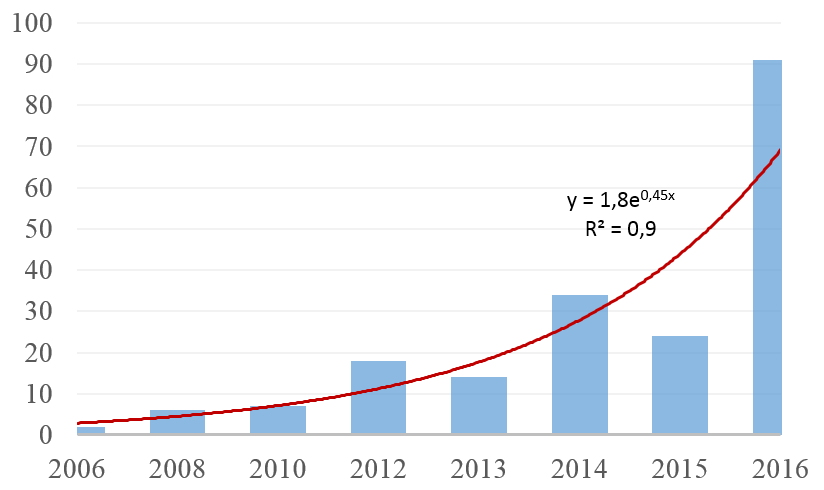
\includegraphics[width=0.8\textwidth]{om5}
  \label{fig:om5}
\end{figure}  

Экспоненциальный рост публикаций в одном издании не может продолжаться бесконечно. 
Каждое издание имеет свой предельный объем публикаций, рукописи, поступающие сверх допустимого изданием объема публикаций, повышают конкуренцию за право быть опубликованным. 
Но в результате отбора некоторые качественные рукописи отвергаются издателями.
Для изучения процесса публикации была разработана имитационная модель. 
Когнитивная карта модели процесса публикаций приведена на рисунке (Рис. \ref{fig:om6}).

\begin{figure}[H]
  \caption{Когнитивная карта модели процесса публикаций.}
  \centering
    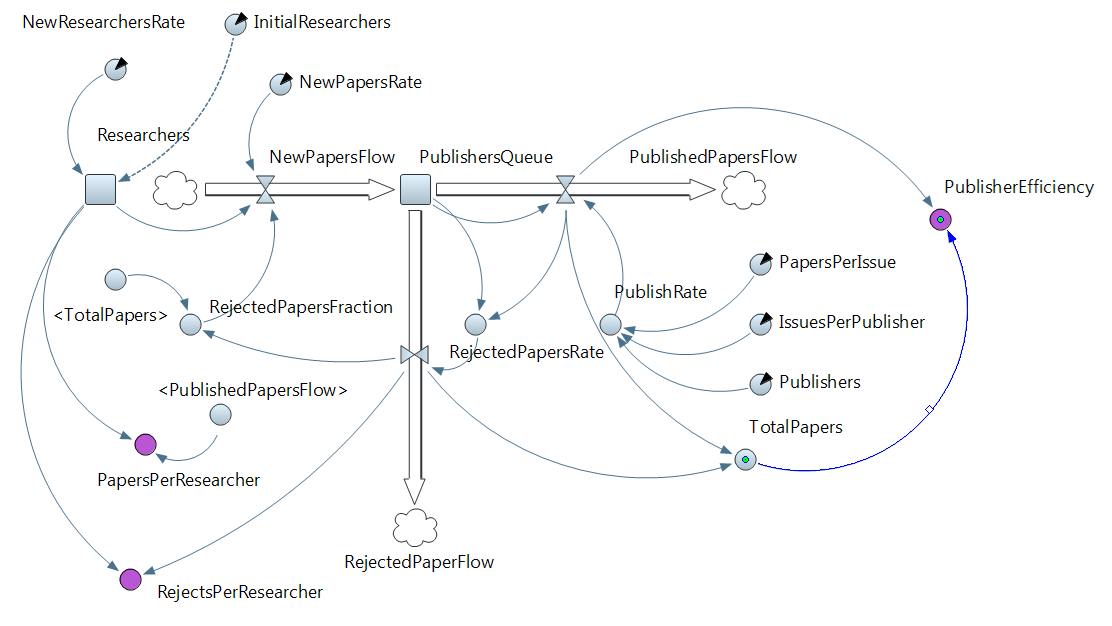
\includegraphics[width=0.8\textwidth]{om6}
  \label{fig:om6}
\end{figure} 

Созданная модель процесса публикаций содержит два накопителя:
\begin{itemize}
\tightlist
\item Researchers — исследователи,
\item PublishersQueue — очередь рукописей.
\end{itemize}

Модель управляется посредством следующих свободных параметров (Таб. \ref{tab:om3}): 

\begin{table}[H]
\centering
\caption{Свободные параметры модели процесса публикаций.}
\label{tab:om3}
\resizebox{\textwidth}{!}{%
\begin{tabular}{|l|l|}
\hline
\textbf{Название параметра} & \textbf{Описание} \\ \hline
Publishers & Количество издателей \\ \hline
PapersPerIssue & Количество статей в выпуске \\ \hline
IssuesPerPublisher & Количество выпусков на одного издателя в год \\ \hline
NewPapersRate & Скорость создания рукописей \\ \hline
InitialResearchers & Начальное количество исследователей \\ \hline
NewResearchersRate & Скорость появления новых исследователей \\ \hline
\end{tabular}%
}
\end{table}

На основании когнитивной карты модели процесса публикаций был проведен цифровой эксперимент.
На рисунке (Рис. \ref{fig:om7}) представлена зависимость эффективности публикаций от времени при различном количестве издателей.

\begin{figure}[H]
  \caption{Кривая зависимости эффективности публикаций от времени при различном количестве издателей (1,3,5,7).}
  \centering
    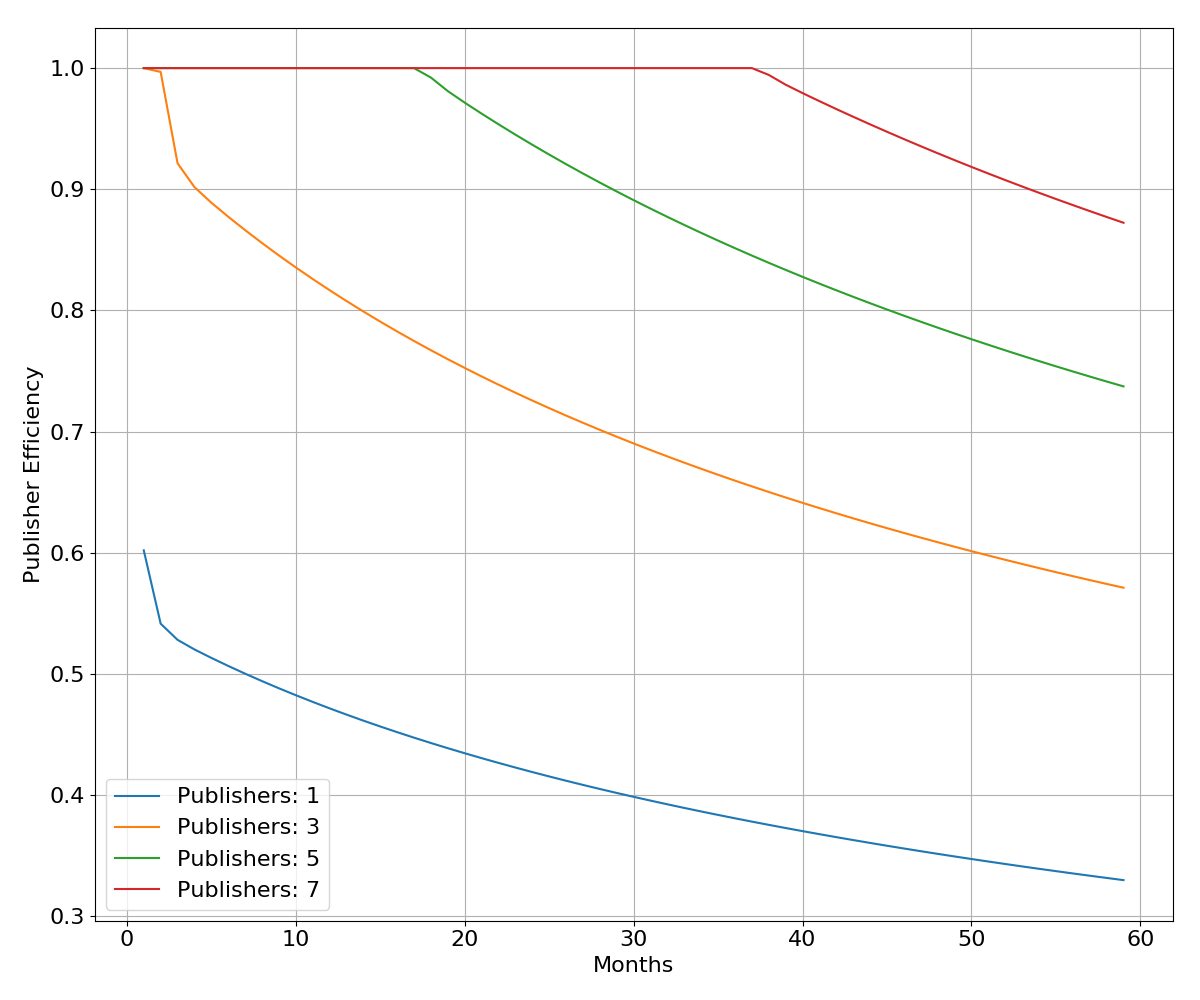
\includegraphics[width=0.8\textwidth]{om7}
  \label{fig:om7}
\end{figure} 

Падение эффективности публикаций как мы видим имеет резкий, лавинообразный характер. 
Такой характер поведения эффективности публикаций требует особого внимания, чтобы не пропустить начало стагнации и принять организационные меры для расширения количества издателей, участвующих в процессе публикации.  

Принцип разделения труда ведет к повышению эффективности процессов. 
Гипотетически расширение ролевой модели может повысить эффективность процесса публикаций. 
Независимо от количества соавторов процесс публикации определяет следующие роли: 

\begin{itemize}
\tightlist
\item Продюсер — носитель основной идеи исследования
\item Редактор — изменяет текст рукописи
\item Рецензент — диалектическая противоположность Продюсера, оппонирует, отвечает за выводы и результаты исследования
\item Переводчик — если статья не на родном языке авторов, то требуется технический перевод и вычитка
\item Специалист по работе с издателями — отвечает за поиск издателей и внешние коммуникации
\item Дизайнер — картинки, презентация для доклада
\item Докладчик — представляет результат в устном виде на конференции (если нужно и столько сколько нужно раз)
\item Исследователь данных — проведение компьютерных расчетов.
\end{itemize}

С учетом перечисленных ролей научно-исследовательская команда не изменяется.
Авторами исследования остаются именно те ученые, которые его провели. 
Повышается качество рукописи, а коммуникации становятся более профессиональными. 
Отметим, что функции внешних и внутренних корпоративных коммуникаций обычно присутствуют в организационной среде, но не имеют фокусировки на работу с индивидуальными потребностями исследователей.

\section{Измерение интеллектуального капитала НТЦ}
\label{sec:ic}
Интеллектуальный капитал (ИК) по своей природе является составным показателем продуктивности научно-исследовательской организации основным продуктом которой являются знания. В структуру ИК входят:
\begin{itemize}
\tightlist
\item Человеческий капитал 
\item Организационный капитал 
\end{itemize}

Человеческий капитал (ЧК) - включает в себя знания и навыки. 
Организационный капитал (ОК) включает в себя технологии и процессы. 
Другими словами, ЧК характеризует опыт сотрудников, а ОК характеризует то как сотрудники применяют свой опыт к поставленным задачам в данной организации. 

Помимо создания интеллектуального капитала  можно рассмотреть и его разрушение – сотрудники, которые вели исследования увольняются и уносят с собой знания.

Вклад сотрудников в интеллектуальный капитал не равнозначен. 
Далее авторы определяют роли, которые относят к ``ядру команды''. 
Потеря сотрудников, состоящих в ядре команды драматически сказывается на производительности. 
К ядру относят сотрудников с высоким уровнем опыта и наиболее востребованными в организации навыками.

Существует достаточно много подходов, описывающих жизненный цикл сотрудника внутри организации или должности , однако большинство исследований соглашается в выделении 4 основных этапов относительно уровня продуктивности:

\begin{enumerate}
\tightlist
\item начальный этап, 
\item накопление опыта, 
\item продуктивный этап, 
\item спад продуктивности.  
\end{enumerate}

При этом этап адаптации (начальный этап и накопление опыта) может отличаться в зависимости от вида деятельности и уровня позиции, но в среднем для специалистов и руководителей среднего звена занимает до полугода, около года для руководителей высшего звена.

Наибольший процент увольнений среди новичков, поэтому больше внимания необходимо уделять социальной адаптации новых сотрудников, встраиванию новичков в процессы и наставничеству.

При распаде творческой команды утечка мозгов бывает разная и не всегда наносит вред производительности. 
Другими словами, иногда уход опытного, но имеющего отличную от большинства ментальную модель сотрудника, уменьшает сдерживающие факторы роста ИК.

Существуют понятия текучести кадров ``по собственному желанию'' и ``по инициативе организации''. 
С точки зрения ИК обе составляющие имеют негативное влияние. 
В Российской практике сложилось устойчивое понятие ``текучести кадров'': показатель, фиксирующий уровень изменения состава вследствие увольнения и перехода на другую работу по личным мотивам. 
В понятие текучести обычно не включают переход сотрудника к другому работодателю через перевод, что сильно искажает российские результаты по сравнению с иностранными. В разных индустриях и сферах промышленности, а также на разных уровнях управления ``нормой'' считают различные значения текучести персонала (от 2-5 до 80\%), что обусловлено особенностями бизнеса и категориями сотрудников. 
Так, например, для розничной торговли и массовой сферы обслуживания характерны самые высокие показатели, тогда как для тяжелой промышленности в целом нормальные достаточно низкие значения (5-10\%).
В целом, можно отметить, что уровень текучести повышается по мере выхода на работу более молодых поколений Х, Y.

Важно так же отметить связь выгорания, усталости и текучести персонала, что имеет негативное воздействие на продуктивность организации.
Положительной обратной связью обладают текучесть кадров и уменьшение производительности труда. 
Организации с высокой текучестью кадров обычно испытывают больше проблем с производительностью труда и с накоплением ИК. 

Наиболее значимой составляющей ИК является продуктивность организации, отражающая отношение эффективного персонала к общему числу сотрудников.  

Автор данного исследования построил модель ИК на основе продуктивности организации. 
Для этого была создана модель численности персонала. 
Модель численности обычно решает задачи прогнозирования численности персонала в зависимости от определенных драйверов численности, как правило, внешних (количество проектов, задач, клиентов, объектов обслуживания) на основе, текущей или заданной производительности труда.
Основной проблемой моделей численности, разрабатываемых организациями, является линейные зависимости численности от драйверов и отсутствие учета фактора адаптации персонала (то есть перехода от новичков к опытным сотрудникам), а также применимость только в конкретной организации с ее драйверами/процессами.

Задачей данного эксперимента является рассмотрение поведения ИК в условиях нагрузки на персонал. 
Для оценки изменений ИК в условиях нагрузки была создана модель выполнения заданий. 
Обе модели в отдельности и общая модель ИК, построенная ни их взаимодействии описаны далее. 

На рисунке (Рис.\ref{fig:icmon1}) приведена когнитивная карта модели численности персонала, разработанная автором данного исследования по рекомендациям из \cite{oliva2010d} .

\begin{figure}[H]
  \caption{Когнитивная карта модели численности персонала.}
  \centering
    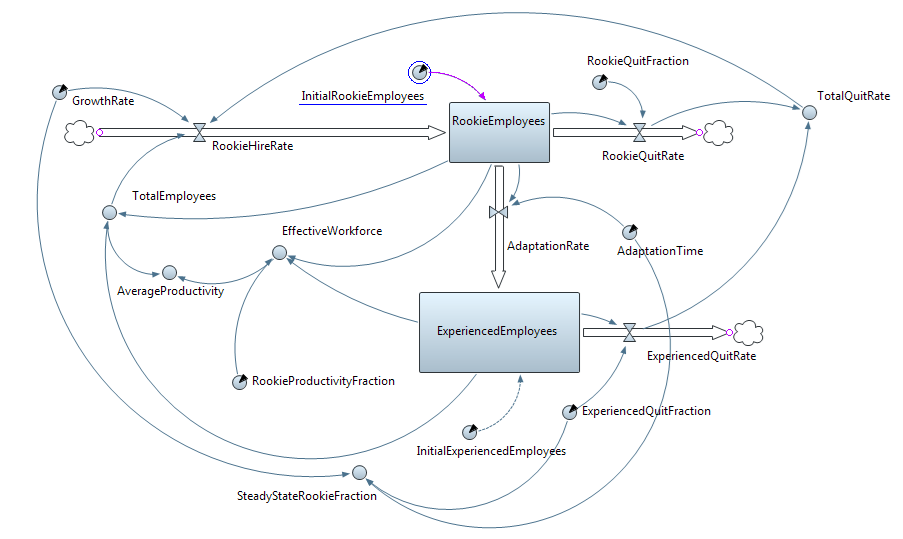
\includegraphics[width=0.8\textwidth]{icmon1}
  \label{fig:icmon1}
\end{figure}  

Модель численности персонала состоит из двух накопителей – Rookie Employees (Новички) и Experienced Employees (Опытные сотрудники) и четырех потоков: 

\begin{itemize}
\tightlist
\item Набор новичков (RookieHireRate),
\item Увольнение новичков (RookieQuitRate),
\item Адаптация новичков в опытных сотрудников (AdaptationRate),
\item Увольнение опытных сотрудников (ExperiencedQuitRate).
\end{itemize}

Свободные параметры модели численности персонала приведены в таблице \ref{tab:icmon1}: 

\begin{table}[H]
\centering
\caption{Свободные параметры модели численности персонала.}
\label{tab:icmon1}
\resizebox{\textwidth}{!}{%
\begin{tabular}{|l|l|l|}
\hline
\textbf{Название параметра} & \textbf{Обозначение параметра} & \textbf{Значение параметра} \\ \hline
Скорость набора персонала & Growth Rate & 0.01 в неделю (от Total Employees) \\ \hline
Начальное количество новичков в компании & Initial Rookie Employees & 40 человек \\ \hline
Начальное количество опытных сотрудников в компании & Initial Experienced Employees & 60 человек \\ \hline
Время адаптации новичка в опытного сотрудника & Adaptation Time & 50-100 недель \\ \hline
Доля вклада новичка в продуктивность персонала & Rookie Productivity Fraction & 30-80\% \\ \hline
Доля увольнений новичков & Rookie Quit Rate & 0.01 \\ \hline
Доля увольнений опытных сотрудников & Experienced Quit Fraction & 0.004 \\ \hline
\end{tabular}%
}
\end{table}

Динамические переменные модели численности персонала перечислены в Таблице Таб. \ref{tab:icmon2}: 

\begin{table}[H]
\centering
\caption{Динамические переменные модели численности персонала }
\label{tab:icmon2}
\resizebox{\textwidth}{!}{%
\begin{tabular}{|l|l|l|}
\hline
\textbf{Название переменной} & \textbf{Обозначение} & \textbf{Формула} \\ \hline
Общее количество сотрудников & Total Employees & RookieEmployees+ExperiencedEmployees \\ \hline
Эффективное количество сотрудников & Effective Workforce & ExperiencedEmployees + RookieProductivityFraction * RookieEmployees \\ \hline
Средняя продуктивность & Average Productivity & EffectiveWorkforce / TotalEmployees \\ \hline
Устойчивая доля новичков & Steady State Rookie Fraction & AdaptationTime*(ExperiencedQuitFraction+GrowthRate)/(1+AdaptationTime*(ExperiencedQuitFraction+GrowthRate)) \\ \hline
Скорость увольнений & Total Quit Rate & RookieQuitRate+ExperiencedQuitRate \\ \hline
\end{tabular}%
}
\end{table}

Потоки перечисленные выше вычисляются по формулам, приведенным в Таблице  \ref{tab:icmon3}: 

\begin{table}[H]
\centering
\caption{Формулы потоков модели численности персонала.}
\label{tab:icmon3}
\resizebox{\textwidth}{!}{%
\begin{tabular}{|l|l|}
\hline
\textbf{Название потока} & \textbf{Формула} \\ \hline
Набор новичков & RookieHireRate = TotalQuitRate + TotalEmployees*GrowthRate \\ \hline
Увольнение новичков & RookieQuitRate = RookieEmployees*RookieQuitFraction \\ \hline
Адаптация новичков в опытных сотрудников & AdaptationRate = RookieEmployees/AdaptationTime \\ \hline
Увольнение опытных сотрудников & ExperiencedQuitRate = ExperiencedEmployees*ExperiencedQuitFraction \\ \hline
\end{tabular}%
}
\end{table}

Для моделирования нагрузки модель численности персонала может быть дополнена процессами выполнения заданий. 
На Рис. \ref{fig:icmon2}  приведена когнитивная карта модели выполнения заданий, разработанная авторами данного исследования.

\begin{figure}[H]
  \caption{Когнитивная карта модели выполнения заданий.}
  \centering
    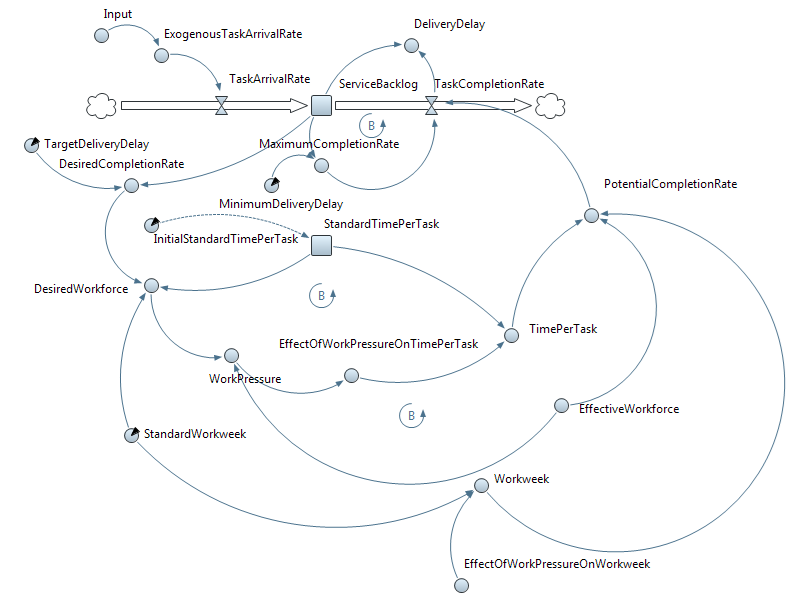
\includegraphics[width=0.8\textwidth]{icmon2}
  \label{fig:icmon2}
\end{figure}  

Модель выполнения заданий состоит из двух накопителей: ServiceBacklog (очередь заданий) и StandardTimePerTask (Стандартное время на выполнение задания). 
Модель выполнения заданий управляется свободными параметрами, приведенными в Таблице \ref{tab:icmon4}:

\begin{table}[H]
\centering
\caption{Свободные параметры модели выполнения заданий.}
\label{tab:icmon4}
\resizebox{\textwidth}{!}{%
\begin{tabular}{|l|l|l|}
\hline
\textbf{Название параметра} & \textbf{Обозначение параметра} & \textbf{Значение параметра} \\ \hline
Стандартная рабочая неделя & Standard Workweek & 40 часов \\ \hline
Целевая задержка исполнения задания & Target Delivery Delay & 0.2 недель \\ \hline
Начальное время выполнения задания & Initial Standard Time Per Task & 1 человек*час/задание \\ \hline
Минимальная задержка выполнения задания & Minimum Delivery Delay & 0.05 недель \\ \hline
\end{tabular}%
}
\end{table}

Динамические переменные модели выполнения заданий приведены в Таблице \ref{tab:icmon5}:

\begin{table}[H]
\centering
\caption{Динамические переменные модели выполнения заданий.}
\label{tab:icmon5}
\resizebox{\textwidth}{!}{%
\begin{tabular}{|l|l|l|}
\hline
\textbf{Название переменной} & \textbf{Обозначение} & \textbf{Формула} \\ \hline
Необходимое количество сотрудников & Desired Workforce & DesiredCompletionRate * StandardTimePerTask / StandardWorkweek \\ \hline
Потенциальная скорость выполнения заданий & Potential Completion Rate & EffectiveWorkforce * Workweek / TimePerTask \\ \hline
Время затраченное на выполнение задания & Time Per Task & StandardTimePerTask * EffectOfWorkPressureOnTimePerTask(WorkPressure) \\ \hline
Требуемая скорость выполнения заданий & Desired Completion Rate & ServiceBacklog / TargetDeliveryDelay \\ \hline
Степень нагрузки на персонал & WorkPressure & DesiredWorkforce / EffectiveWorkforce \\ \hline
Рабочая неделя & Workweek & StandardWorkweek * EffectOfWorkPressureOnWorkweek(WorkPressure) \\ \hline
\end{tabular}%
}
\end{table}

Очередь заданий (ServiceBacklog) управляется экзогенной динамическим потоком поступления новых заданий (TaskArrivalRate) и потоком выполненных заданий (TaskCompletionRate). 
Точка равновесия для модели выполнения заданий  определена следующим уравнением (\ref{eq:icmon1}):

\begin{equation}
EffectiveWorkforce = Desired Workforce
\label{eq:icmon1}
\end{equation}

Модель численности персонала представляет основу для модели выполнения заданий. 
Вместе эти модели представляют динамику навыков и процессов, что характеризует интеллектуальный капитал организации, как мы уже отмечали ранее.
Модели соединены динамическими переменными, приведенными в Таблице \ref{tab:icmon6}:

\begin{table}[H]
\centering
\caption{Динамические переменные, объединяющие модель численности персонала и модель выполнения заданий.}
\label{tab:icmon6}
\resizebox{\textwidth}{!}{%
\begin{tabular}{|l|l|l|}
\hline
\textbf{Название переменной} & \textbf{Обозначение} & \textbf{Описание действия} \\ \hline
Эффективное количество сотрудников & Effective Workforce & Вычисляется в модели численности персонала для модели выполнения заданий. Описывает количество сотрудников для выполнения заданий. \\ \hline
Рабочая неделя & Workweek & Вычисляется в модели выполнения заданий для модели численности персонала. Описывает количество часов требуемых для выполнения поступающих заданий. \\ \hline
\end{tabular}%
}
\end{table}

Для выявления поведения ИК исследуем кривые производительности. 
Кривая производительности является графическим представление изменения скорости обучения определённому виду деятельности. 
На рисунке \ref{fig:icmon3} приведены кривые производительности для модели численности персонала при различных значениях времени адаптации новичков. 
В модели численности персонала динамической переменной, характеризующей производительности, является Средняя продуктивность персонала (Average Productivity).

\begin{figure}[H]
  \caption{Кривые производительности для различных значений Времени адаптации новичков.}
  \centering
    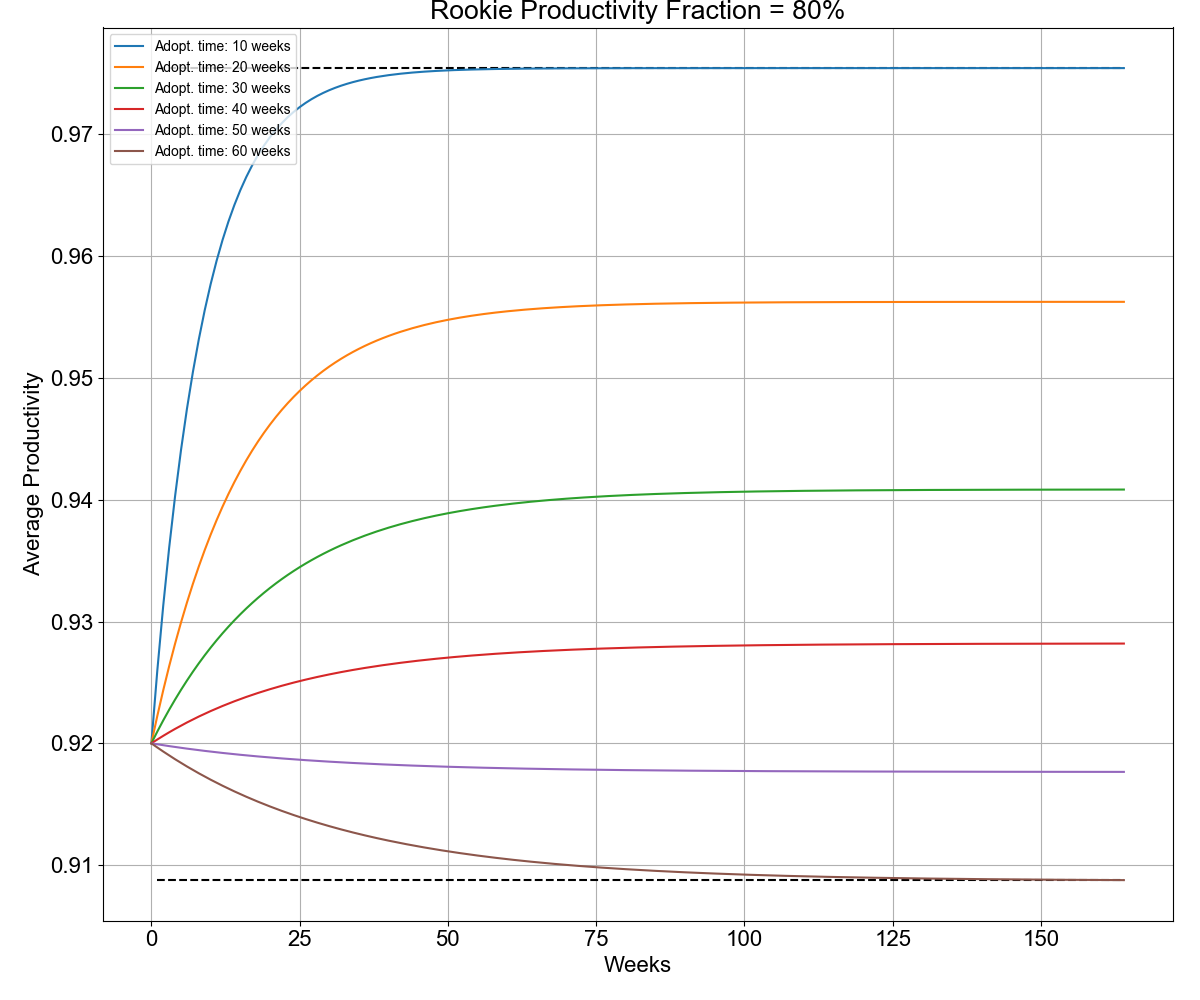
\includegraphics[width=0.8\textwidth]{icmon3}
  \label{fig:icmon3}
\end{figure}  

Как мы видим из рисунка \ref{tab:icmon3} для Доли вклада новичка равной 80\% при временах адаптации более 50 недель кривая обучаемость стремиться к нижней асимптоте, а при временах более 60 недель стремиться к верхней асимптоте Средней продуктивности. 
Таким образом, демонстрируя разный характер поведения. 
На практике это означает, что при значительном времени адаптации новичков организационная производительность падает, так как количество опытных сотрудников в коллективе уменьшается по отношению к новичкам, а вклад в продуктивность от новичков меньше чем от опытных сотрудников. 

С другой стороны, из кривых на рисунке \ref{fig:icmon4} видно, что для Времени адаптации равному 20 неделям кривые продуктивности имеют единый характер и отличаются скоростью выхода на предельное значение – асимптоту. 

\begin{figure}[H]
  \caption{Кривые производительности для различных значений Доли вклада новичков.}
  \centering
    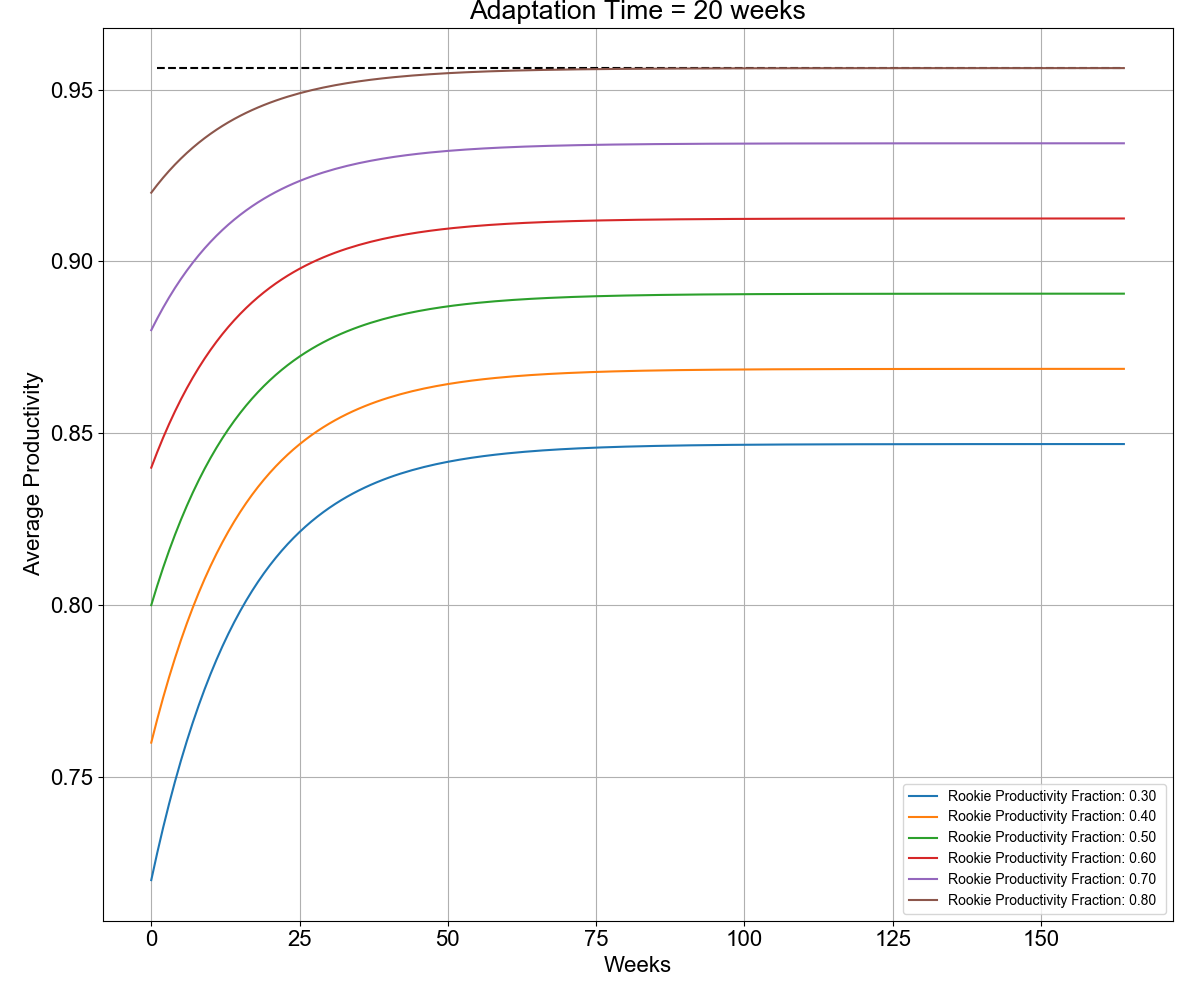
\includegraphics[width=0.8\textwidth]{icmon4}
  \label{fig:icmon4}
\end{figure} 

Небольшие Доли вклада новичков означают, что сложность заданий не подразумевает участия в них неподготовленных сотрудников. 
С другой стороны, большие Доли вклада новичков означают, что задания позволяют даже неопытному сотруднику работать с высокой отдачей, приближающейся к отдачи опытных сотрудников.

Для моделирований ИК под нагрузкой мы будем использовать экзогенную функцию для потока заданий (Рис. \ref{fig:icmon5}), для создания разных нагрузок.

\begin{figure}[H]
  \caption{Кривые производительности и нагрузки для модели ИК.}
  \centering
    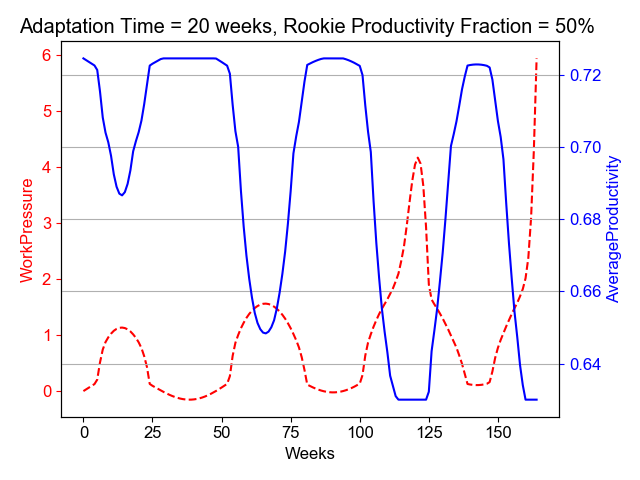
\includegraphics[width=0.8\textwidth]{icmon5}
  \label{fig:icmon5}
\end{figure} 

Из рисунка \ref{fig:icmon5} мы видим, что в пиковых нагрузках производительность падает, но за счет адаптации новичков организация, восстанавливает производительность, когда нагрузка спадает. 
Для различных времен адаптации в модели ИК кривые производительности будут иметь вид, представленный на рисунке (Рис. \ref{fig:icmon6}).

\begin{figure}[H]
  \caption{Кривые производительности для различных значений Времени адаптации новичков с учетом нагрузки.}
  \centering
    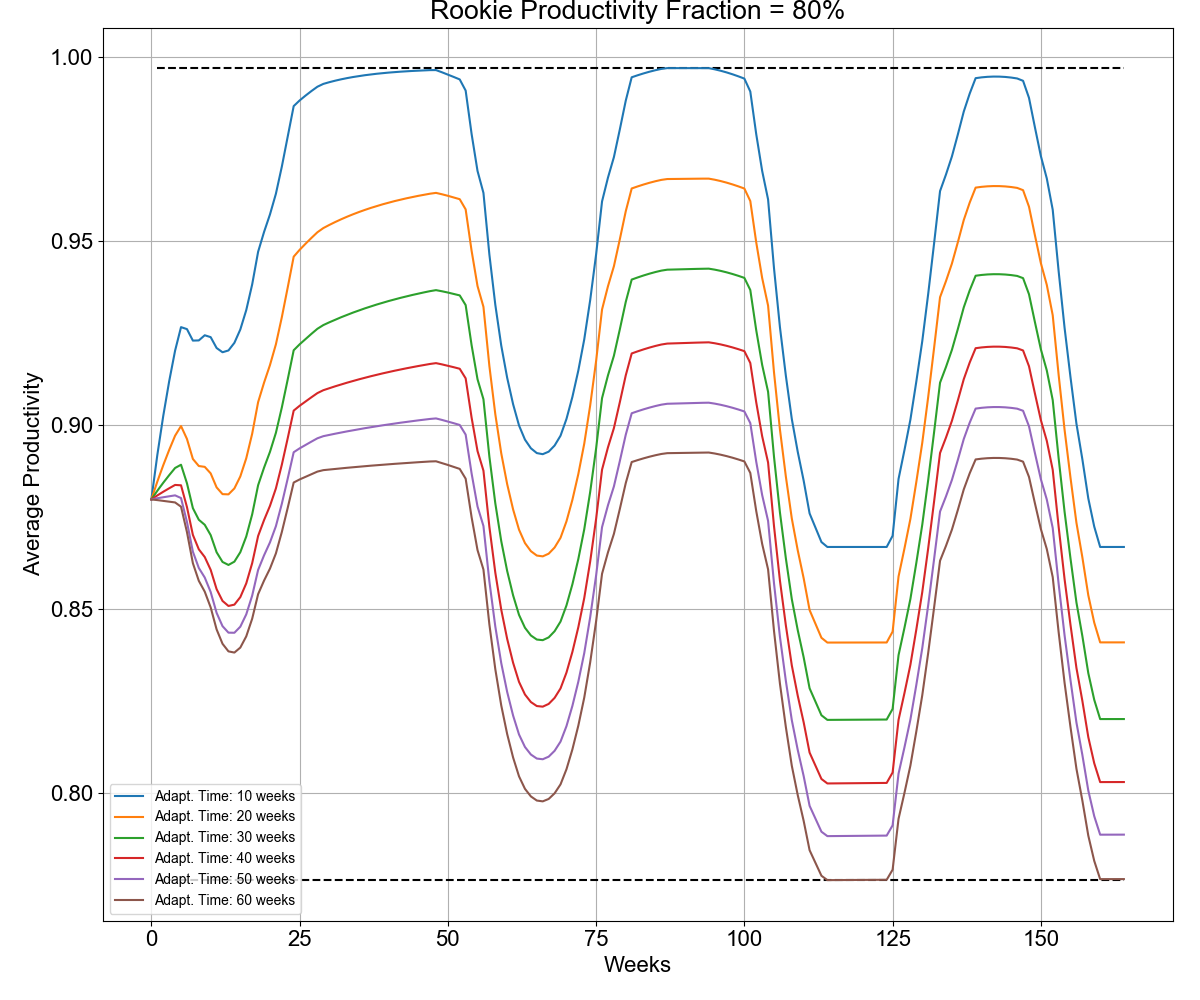
\includegraphics[width=0.8\textwidth]{icmon6}
  \label{fig:icmon6}
\end{figure} 

На рисунке (Рис.\ref{fig:icmon7})  представлены кривые производительности для Времени адаптации равному 20 неделям с учетом нагрузки. 
Мы можем наблюдать различное поведение производительности до выхода на асимптоты при различных долях участия новичков, что отражает тот факт, что возможное включении новичков в решение заданий (до адаптации) характеризует эти задания, как достаточно простые и типовые.

\begin{figure}[H]
  \caption{Кривые производительности для различных значений Доли вклада новичков с учетом нагрузки.}
  \centering
    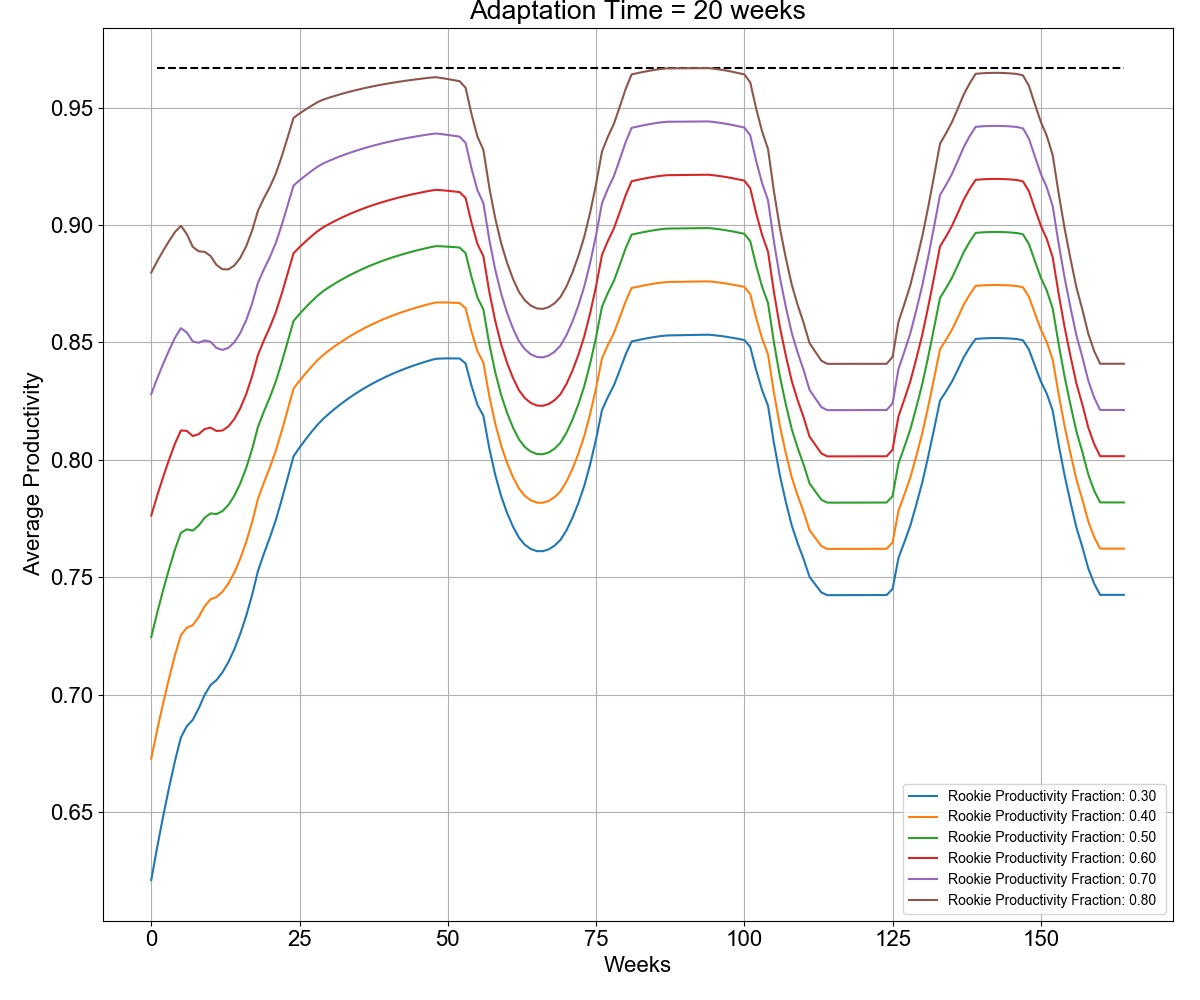
\includegraphics[width=0.8\textwidth]{icmon7}
  \label{fig:icmon7}
\end{figure} 

Отметим, что при небольшом времени адаптации новичков (20 недель) и высокой доли участия новичков в продуктивности (80\%) относительное падение продуктивности ниже, чем при невысокой высокой доли участия новичков в продуктивности (30\%). 
Это наблюдение подтверждает тот факт, что при возрастании нагрузки коротких и простых заданий для новичков их продуктивность падает меньше, чем на сложных заданиях.

Для моделирования эффекта ``выгорания'' и ``усталости'' сотрудников в условиях длительной работы в режиме удлинённой недели в модель ИК введены следующие зависимости: 
\begin{enumerate}
\tightlist
\item Эффект ``выгорания'' состоит в увеличении скорости увольнения опытных сотрудников в зависимости от времени работы в условиях удлинённой недели.
\item Эффект ``усталости'' сотрудников состоит в уменьшении производительности сотрудников в зависимости от времени работы в условиях удлинённой недели.
\end{enumerate}

На рисунке (Рис.\ref{fig:icmon8})  изображен результат симуляции модели ИК для 500 недель. Такой длительный срок выбран с целью показать эффекты ``выгорания'' и ``усталости'' персонала и как следствие падение продуктивности вызванной работой в условиях удлинённой рабочей недели.

\begin{figure}[H]
  \caption{Кривые производительности и нагрузки для модели ИК в условиях удлинненой рабочей недели.}
  \centering
    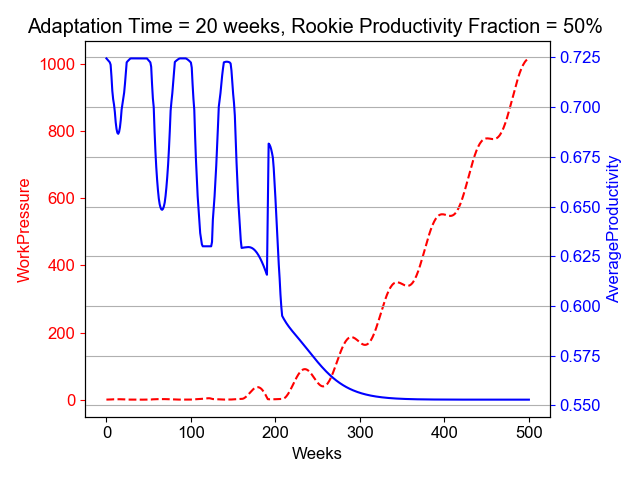
\includegraphics[width=0.8\textwidth]{icmon8}
  \label{fig:icmon8}
\end{figure} 

Падение производительности, вызванное длительной высокой нагрузкой, драматически влияет на ИК. 
В заключение на рисунке (Рис.\ref{fig:icmon9}) представлены кривые изменения человеческого капитала – опытных сотрудников, новичков и общего числа сотрудников. Отдельно приведена кривая требуемого количества сотрудников для выполнения поступающих заданий. 
Мы видим, что количество новичков растет быстрее, чем количество опытных сотрудников.

\begin{figure}[H]
  \caption{Кривые изменения человеческого капитала по модели ИК.}
  \centering
    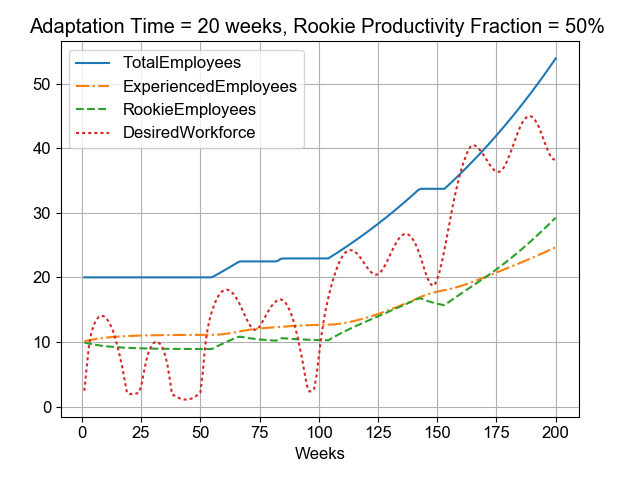
\includegraphics[width=0.8\textwidth]{icmon9}
  \label{fig:icmon9}
\end{figure} 

Приведенные результаты эксперимента подтверждает теоретические работы по изучению процессов управления интеллектуальным капиталом. 
Новизна данного исследования состоит в выработке количественных оценок, помогающих уточнить стратегию управления интеллектуальным капиталом научно-исследовательской организации. 

Рассмотренная автором ситуация работы в условиях высокой нагрузки является типичной для российской экономики в современных условиях и особенно актуально в нефтегазовой отрасли.

\section{Результаты моделирования командообразования в научной деятельности}
\label{sec:so}
Допустим, что в отраслевой научно-исследовательской организации $\Omega$  работают лаборатории $\lambda_i$ , где $i \in (1 \dots N_{\lambda})$ . 
Обозначим множество лабораторий $ \Lambda = \{ \lambda_i, \dots , \lambda_{N_{\Lambda}} \}$.
В лабораториях работают научные сотрудники $ A = \{ a_{i}, \dots, a_{N_A} \} $.  

Обозначим множество тематик $t_i$, где $i \in (1, \dots, N_T )$, по которым организация $\Omega$ ведет НИР как $T = \{ t_1, \dots , t_{N_T} \}$. Тогда деятельность организации $\Omega$ по выполнению НИР может быть описана следующими компонентами (\ref{eq:so1}):
\begin{equation} 
\label{eq:so1}
\mathbb{M}_{\Omega} = \bigg \{ S, \Xi, \Psi, E \bigg \} \mbox {, где}  S = \{ \Lambda, A, T, P, X \}
\end{equation} 

Помимо вышеопределенных компонент в уравнении \ref{eq:so1} присутствуют:

\begin{itemize}
\item $ \Xi = \{ \xi_1 , \dots , \xi_{N_{\Xi}} \} $ -- множество связей между субъектами (знакомство, соавторство и др.),
\item $ \Psi = \{ \psi_1 , \dots , \psi_{N_{\Psi}} \} $ -- множество действий субъектов (``поиск темы'', ``отправка тезисов'' и др.),
\item $ P = \{ \rho_1 , \dots , \rho_{N_P} \} $ -- множество научных работ,
\item $ X = \{ \chi_1 , \dots , \chi_{N_X}  \} $ -- множество научных журналов и конференций.
\end{itemize}

Сотрудники  организации $\Omega$  выполняют НИР по тематикам $T$ , создают научные статьи и доклады $P$ для публикации их в журналах и выступлениях на конференциях $X$.
При создании научных статей $P$ используются обзоры материалов журналов и конференций $X$.
Конференции и редакции журналов $X$ устанавливают приоритетные тематики $T$ и принимают статьи для публикации по определенному графику (тезисы, полный текст, замечания рецензентов, выступление, публикация) и от наиболее квалифицированных и опытных научных работников.
Научный работник обладает квалификациями по тематикам $T$, которые можно представить в виде n-мерного вектора $(c_1, \dots , c_{N_T} )$ и опытом написания статей $(e_1 , \dots , e_{N_E} )$, где $c_i,e_i \in \mathbb{R}$. 
И квалификации, и опыт не нуждаются в нормировке. 
Квалификация растет при успешном выполнении НИР, а опыт растет с успешной публикацией статей по соответствующей тематике.
Имитационное моделирование представляет собой статистический эксперимент. 
Его результаты должны основываться на соответствующих статистических проверках. 
Автор выбрал метод повторения для вычисления доверительных интервалов и проверки гипотез.
Таким образом, каждое наблюдение представляется независимым прогоном модели, в котором переходный период не учитывается.
Далее производится вычисление средних величин выборки. 
Так как, прогоны независимы, то применяется стандартная формула для дисперсии.
Преимуществом данного метода является то, что каждый имитационный прогон модели определяется своей последовательностью случайных чисел из интервала [0;1], что действительно обеспечивает статистическую независимость получаемых наблюдений. 
Недостатком является то, что все наблюдения могут оказаться под сильным влиянием начальных переходных условий.

В качестве калибровки для моделирования взят Газпромнефть НТЦ. 
В рамках НТЦ выбраны шесть тематик исследований $T = \{ t_1, \dots , t_{N_T} \} $ , где $N_T = 6 $ :

\begin{enumerate}
\tightlist
\item Разработка и эксплуатация нефтяных месторождений
\item Геология и геологоразведочные работы
\item Информационные технологии
\item Техника и технология добычи нефти
\item Проектирование обустройства месторождений
\item Бурение скважин
\end{enumerate}

В качестве издателя $\chi_1$ выбрана редакция ``Нефтяное хозяйство'' выпускающая одноименный журнала с 1933 года. Авторы выбрали номер журнала за декабрь 2016 (НХ,12-2016), полностью состоящий из статей сотрудников ``Газпромнефть НТЦ''. В качестве конференции $\chi_2$ выбрана конференция 16RPTC (SPE Russian Petroleum Technology Conference and Exhibition), прошедшая 24 октября 2016 года в Москве. 
Таким образом, $X = \{ \chi_1, \dots , \chi_{N_X} \} $ , где $ N_{X} = 2$.

В настоящее время в анализе социальных коллабораций выделяются два подхода:
\begin{itemize}
\tightlist
\item Структурный подход акцентирует внимание на геометрической форме сети и интенсивности взаимодействий (весе ребер). Для интерпретации результатов в данном случае используются структурные теории и теории сетевого обмена.
\item Динамический подход акцентирует внимание на изменениях в сетевой структуре с течением времени
\end{itemize}

Целью эксперимента  на данном этапе было подтвердить достаточность структуры компонент модели $\mathbb{M}_{\Omega}$ на примере научно-технического центра из нефтегазовой отрасли. При наблюдении визуализации поведения агентов у авторов не возникло необходимости в добавлении новых компонентов в модель.

Для поставленных условий на основании $\mathbb{M}_{\Omega}$ была создана частная модель $\mathbb{M}_{GPN}$  и проведена много прогонная симуляция модели (Рис. \ref{fig:so1}).

\begin{figure}[H]
  \caption{Фрагмент визуализации прогона симуляции частной модели для НТЦ из нефтегазовой отрасли.}
  \centering
    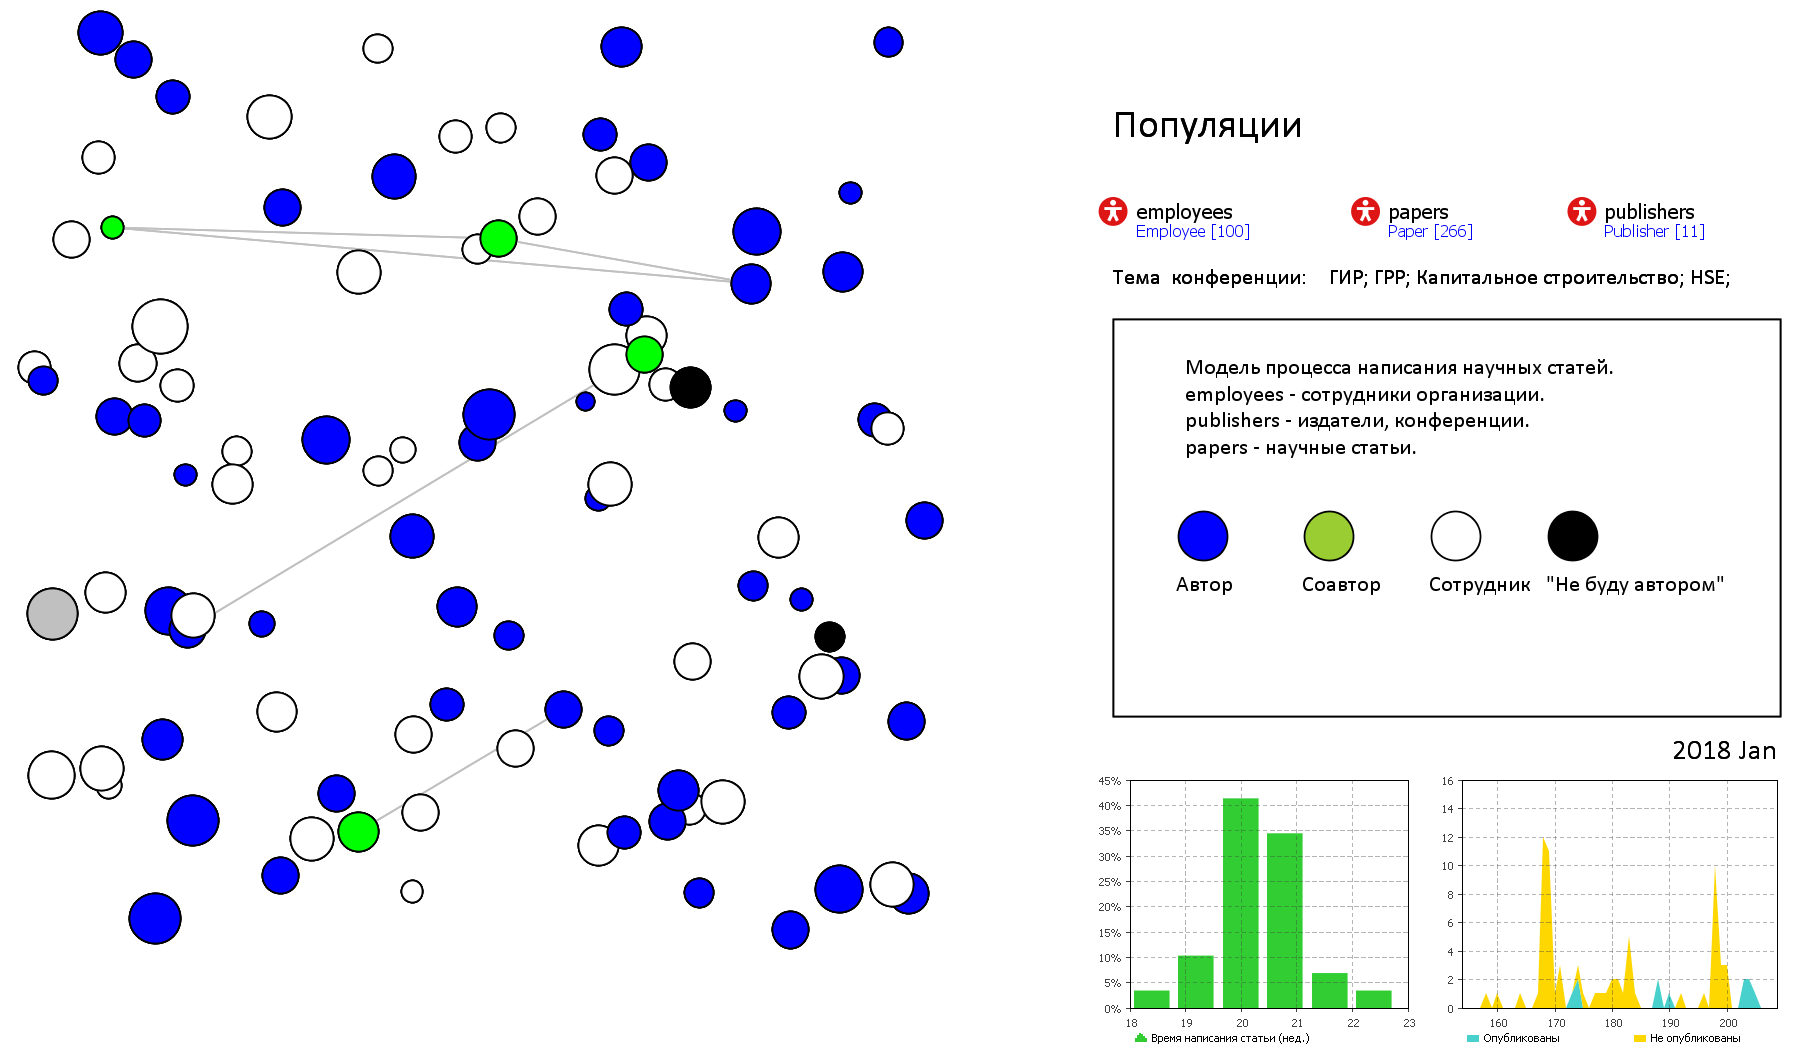
\includegraphics[width=0.8\textwidth]{so1}
  \label{fig:so1}
\end{figure}  

Далее на основании симуляций была создана база данных для последующего исследования процессов.
База данных содержит следующие основные сущности (Рис. \ref{fig:so2}).

\begin{figure}[H]
  \caption{Entity relationship diagram (ERD): Сущности процесса создания научных статей.}
  \centering
    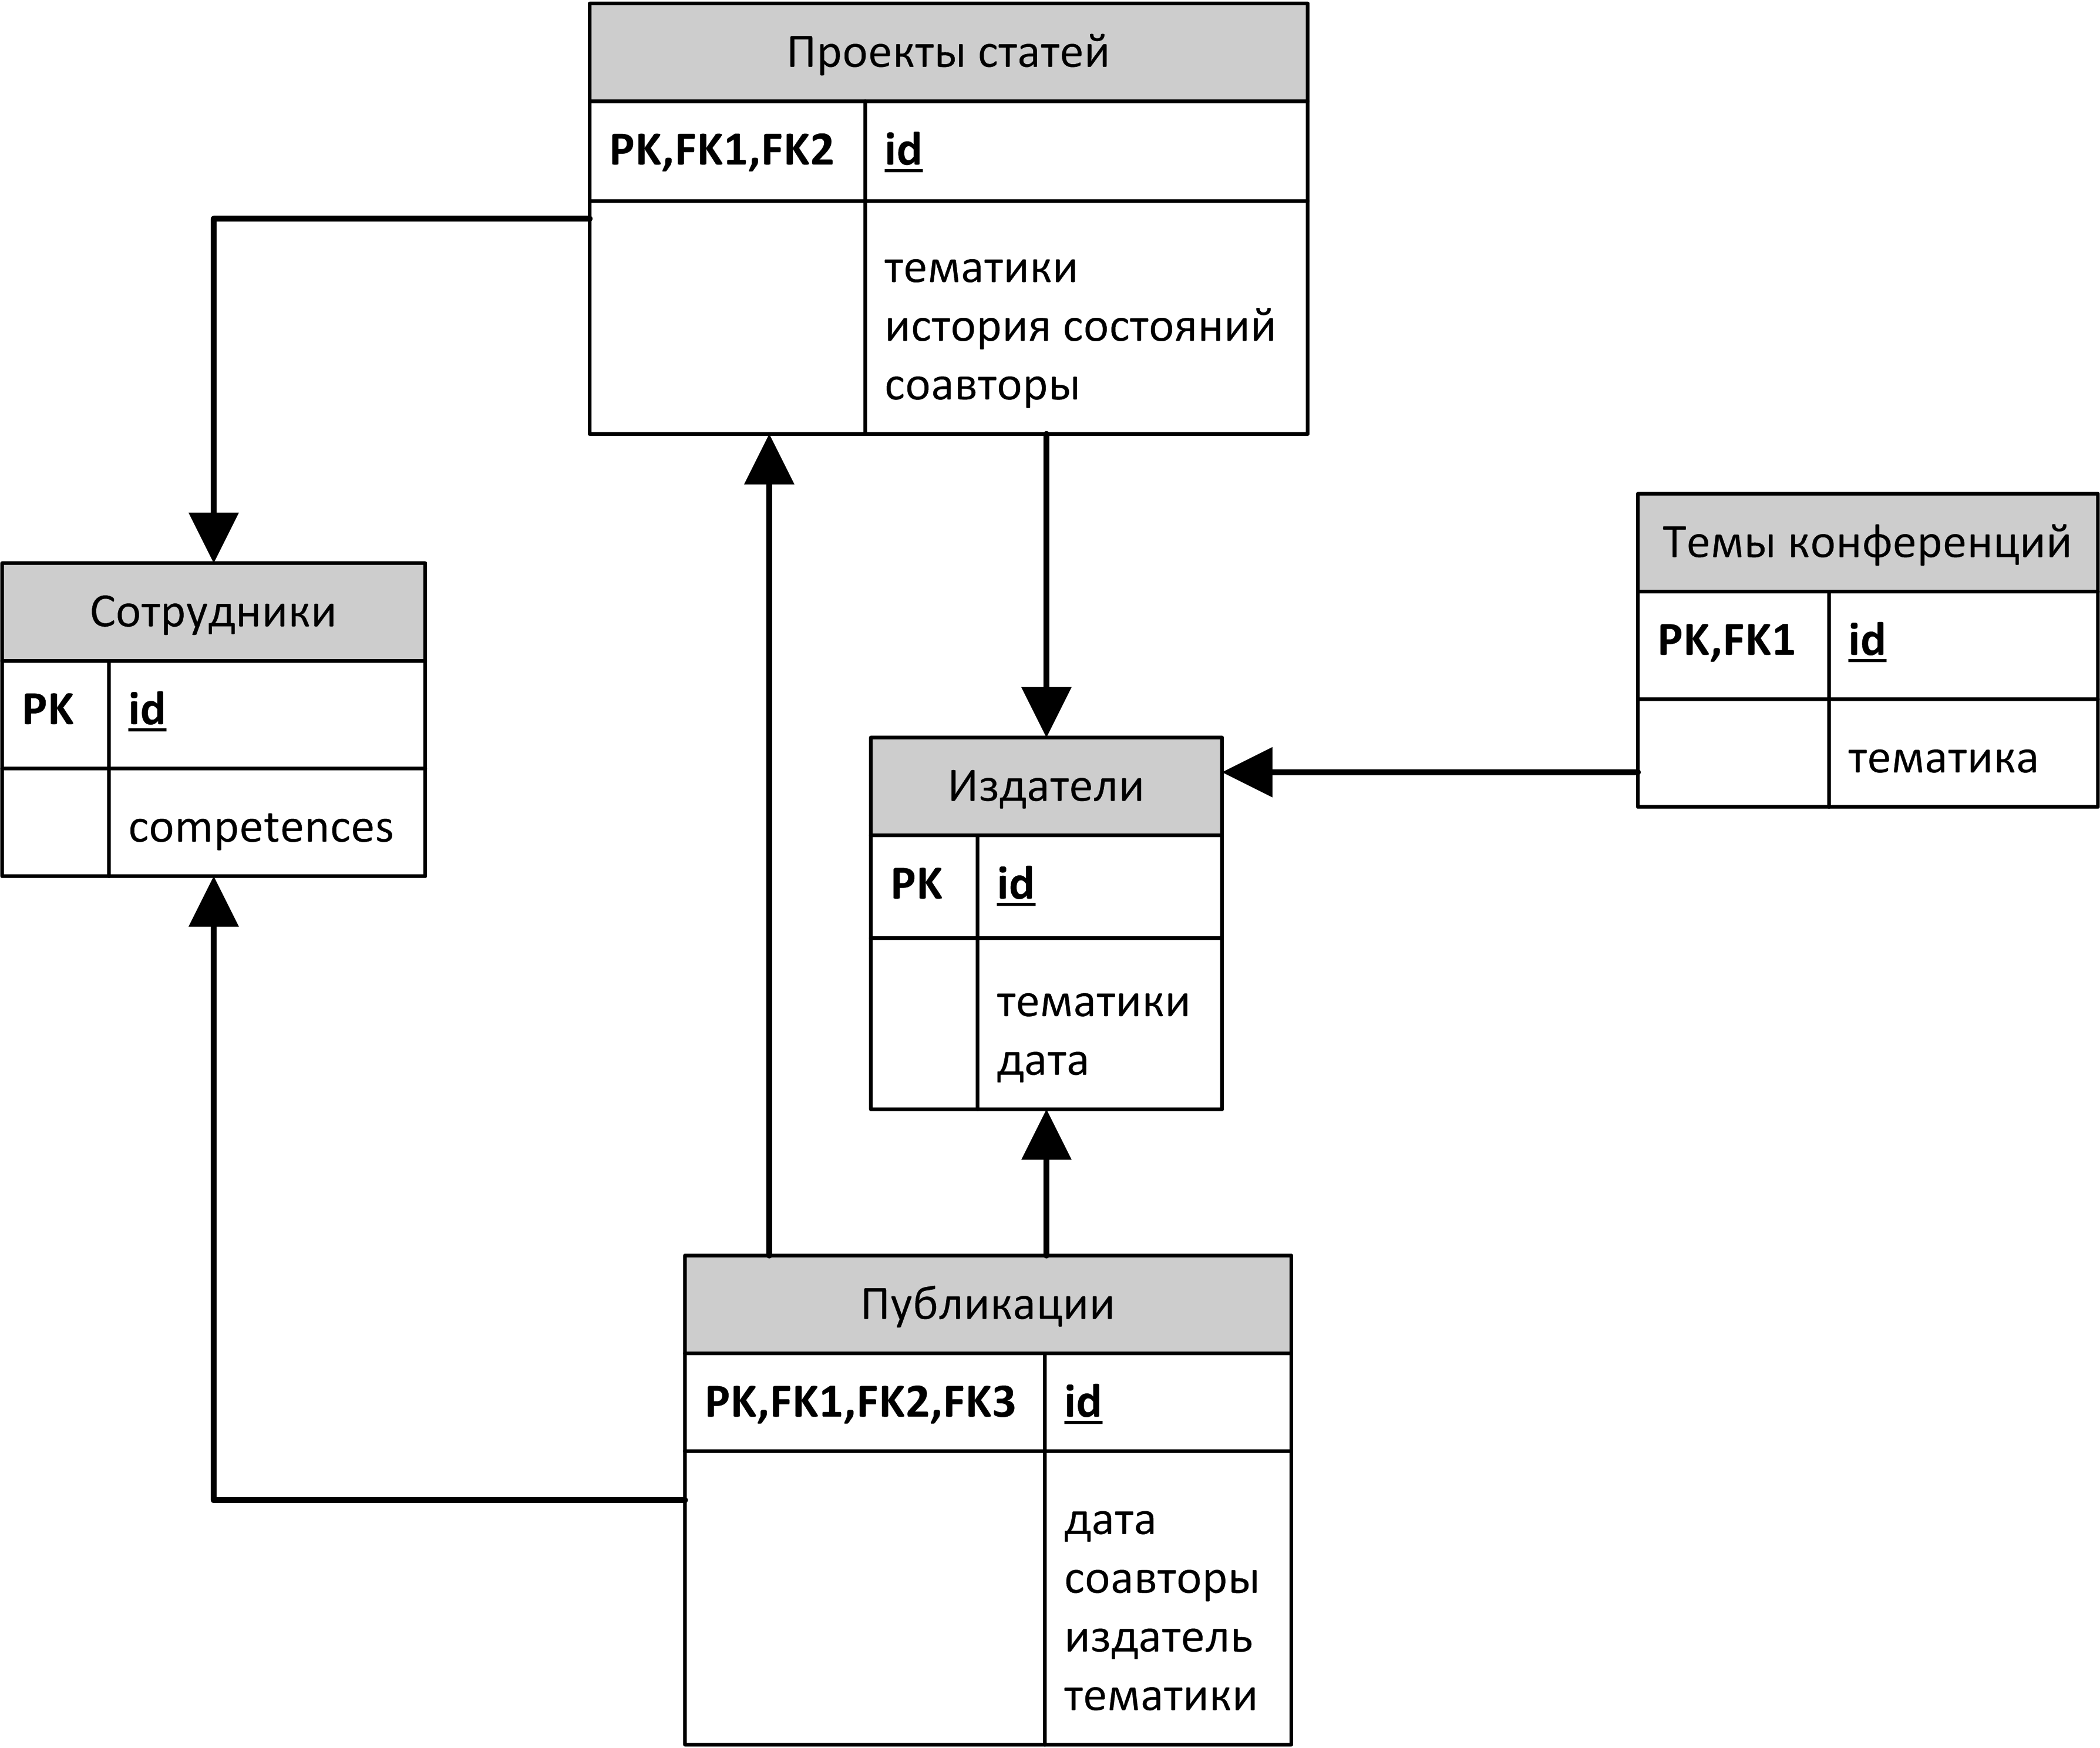
\includegraphics[width=0.8\textwidth]{so2}
  \label{fig:so2}
\end{figure}  

По результатам имитационного моделирования нами были получены следующие результаты для процесса создания и публикации научной статьи:
\begin{enumerate}
\item Среднее время написания статьи: $20 \pm 2$ недель.
\item Среднее число соавторов: $3.5 \pm 1.0$
\item Максимальное число соавторов: $7 \pm 3$
\item Среднее количество статей на одного автора в год: $2 \pm  0.5$
\item Доля статей, не уложившихся в график публикации: $40 \pm 10$ \%.
\end{enumerate}

Данные результаты находятся в согласии с опытом автора, но нуждаются в дальнейшей проверке.
Для оценки корректности результатов моделирования было проведено сопутствующее библиометрическое исследование реальных эмпирических данных по собственной методике автора \cite{KDGY}. 
В соответствии с поставленными условиями эксперимента была создана база публикаций, содержащая следующие информационные поля:

\begin{enumerate}
\tightlist
\item Дата публикации статьи
\item Список авторов
\item Название статьи
\item Тематика статьи согласно классификатору тематик $T$
\item Издатель согласно классификатору $X$
\end{enumerate}

В базу публикаций были собраны статьи издательства ``Нефтяное хозяйство'' и публикации из электронной библиотеки сообщества нефтегазовых инженеров SPE OnePetro, сделанные сотрудниками Газпромнефть НТЦ.
Проведен анализ публикаций и построен граф соавторств (Рис.\ref{fig:so3}).

\begin{figure}[H]
  \caption{Синтетический граф соавторств для НТЦ "Газпромнефть".}
  \centering
    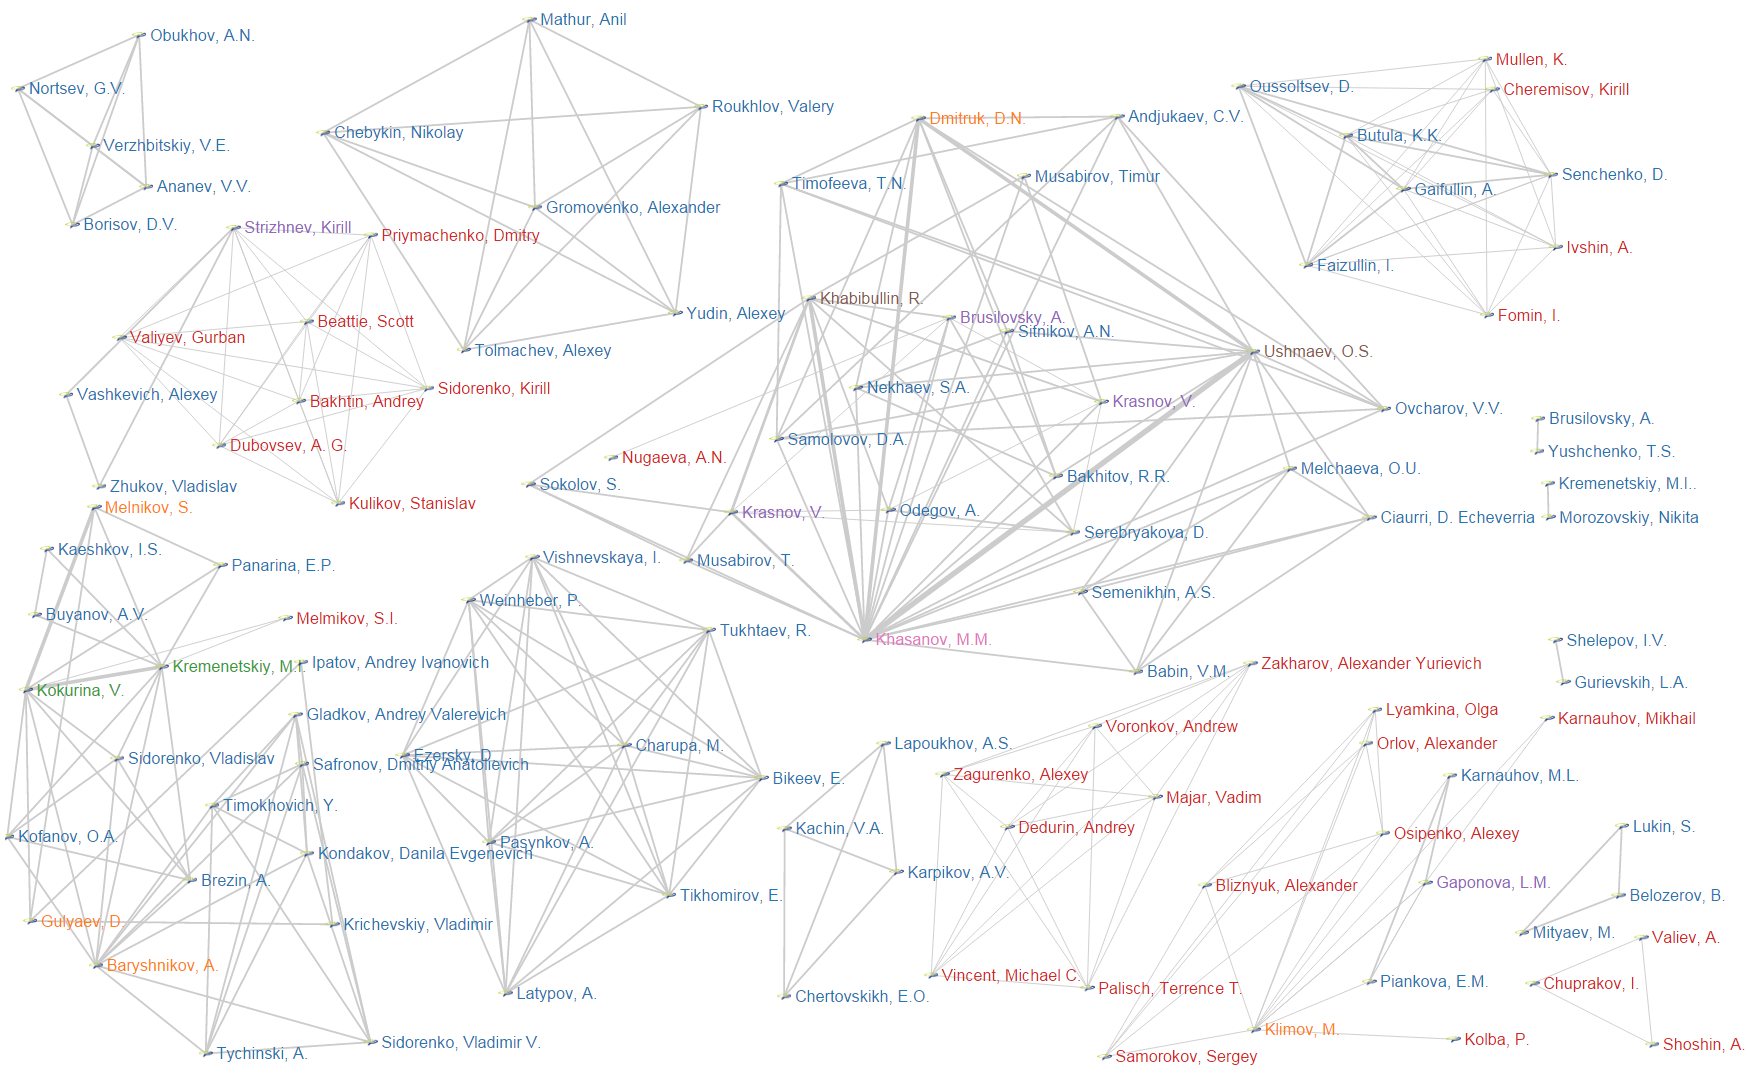
\includegraphics[width=0.8\textwidth]{so3}
  \label{fig:so3}
\end{figure}  

На основании базы публикаций вычислены следующие параметры соавторства:

\begin{enumerate}
\tightlist
\item Среднее количество опубликованных статей на одного автора в год: $ 2 \pm 0.5$
\item Среднее количество соавторов: $2.8 \pm 0.1$
\item Максимальное количество соавторов: $10 \pm 1$
\end{enumerate}

Полученные эмпирические результаты подтверждают результаты имитационного моделирования, что свидетельствует о перспективах применения имитационного моделирования как аналога для моделирования социальных процессов в организационной среде.

\section{Результаты оптимизации процессов научной деятельности}
\label{sec:scrum}
Задача поиска оптимальных параметров команды соавторов для наиболее продуктивного написания научных статей относится к классу задач оптимизации. 
Функция, которую необходимо минимизировать будет зависеть от следующих параметров:

\begin{itemize}
\tightlist
\item
  Количество сотрудников в организационной среде ($N_{o}$);
\item
  Скорость появления новых сотрудников ($Vemp_{new}$);
\item
  Скорость увольнения сотрудников ($Vemp_{fired}$);
\item
  Максимальное количество компетенций у сотрудника ($Cmax_{emp}$);
\item
  Максимальное количество компетенций необходимых для достижения цели исследования ($Cmax_{pub}$).
\end{itemize}

Показателями производительности процесса написания статей, оптимальные значения которых необходимо найти, могут быть следующие:

\begin{itemize}
\tightlist
\item
  Время написания научной статьи ($T_{pub}$)
\item
  Доля сотрудников, опубликовавших статьи от всего количества
  сотрудников ($Frac_{pub}$)
\item
  Доля несостоявшихся статей ($Frac_{notpub}$).
\end{itemize}

Параметрами организационной среды будут следующие:

\begin{itemize}
\tightlist
\item
  Минимальное и максимальное количество сотрудников в организации
  ($N_{omax}$,$N_{omin}$)
\item
  Скорость появления потенциальных целей исследований ($V_{pub}$)
\item
  Временные ограничения на написание статьи ($T_{eoc}$)
\item
  Скорость встреч для заведения знакомств между сотрудниками
  ($V_{friending}$)
\item
  Скорость встреч участников с потенциальными целями
  ($V_{go}$)
\end{itemize}

Исходя из вышеописанных параметров фитнесс-функция $\mathcal{F}$ для оптимизации может быть записана в следующем виде (\ref{eq:scrum5}):

\begin{equation} 
\label{eq:scrum5}
\mathcal{F}\bigg\{ \frac{1}{Frac_{pub}}, T_{pub}, Frac_{notpub} \bigg\} \rightarrow \, min
\end{equation}

При выполнении системы основных условий:

\begin{equation} 
\left\{ \begin{array}{rcl}
N_o \in [ N_{omin}, N_{omax} ]\\ 
Cmax_{emp} \leq Cmax_{pub} \in [ 1, N_{comp} ]\\
Vemp_{new} \geq Vemp_{fired} \geq 0
\end{array}\right.
\label{eq:scrum6}
\end{equation}

Оптимизационный эксперимент был проведен в среде AnyLogic для моделей, с применением Scrum и без. 
Графы соавторств с применением Scrum не изменились.
На основании оптимизационного эксперимента была произведена калибровка имитационной модели соавторства разработанной автором данного исследования. 
Были найдены оптимальные параметры $N_{o}$,$Vemp_{new}$, $Vemp_{fired}$,$Cmax_{emp}$,$Cmax_{pub}$ для Газпромнефть НТЦ. 
Оптимальные значения параметров приведены в Таблице \ref{tab:ex1}.

\begin{table}[H]
\centering
\caption{Оптимальные значения параметров}
\label{tab:ex1}
\resizebox{\textwidth}{!}{%
\begin{tabular}{|l|c|}
\hline
\textbf{Название параметра} & \textbf{Значение параметра} \\ \hline
Количество сотрудников в организационной среде ($N_o$) &  136 \\ \hline
Скорость появления новых сотрудников ($Vemp_{new}$) & 1 сотрудник в неделю \\ \hline
Скорость увольнения сотрудников ($Vemp_{fire}$) & 1 сотрудник в месяц \\ \hline
Максимальное количество компетенций у сотрудника ($Cmax_{emp}$) &  4 \\ \hline
Максимальное количество компетенций необходимых для достижения цели ($Cmax_{pub}$) & 5 \\ \hline
\end{tabular}
}
\end{table}

Калиброванная модель стала основой для исследования эффекта от введения Scrum ролей в процесс написания научных статей.
Для выбранных в разделе показателей производительности $T_{pub}$ и $Frac_{notpub}$ была проведена много прогонная симуляция двух типов: с использованием методики Scrum и без Scrum. 
Анализ данных был произведен в статистической среде $R$.

Результаты попрогонного изменения $T_{pub}$ и $Frac_{notpub}$ приведены на рисунках \ref{ex:fig12} и \ref{ex:fig13} соответственно.
\begin{figure}[H]
  \caption{ Среднее время публикации статей в зависимости от номера прогона. Линиями нарисована зависимость скользящего среднего.}
  \centering
    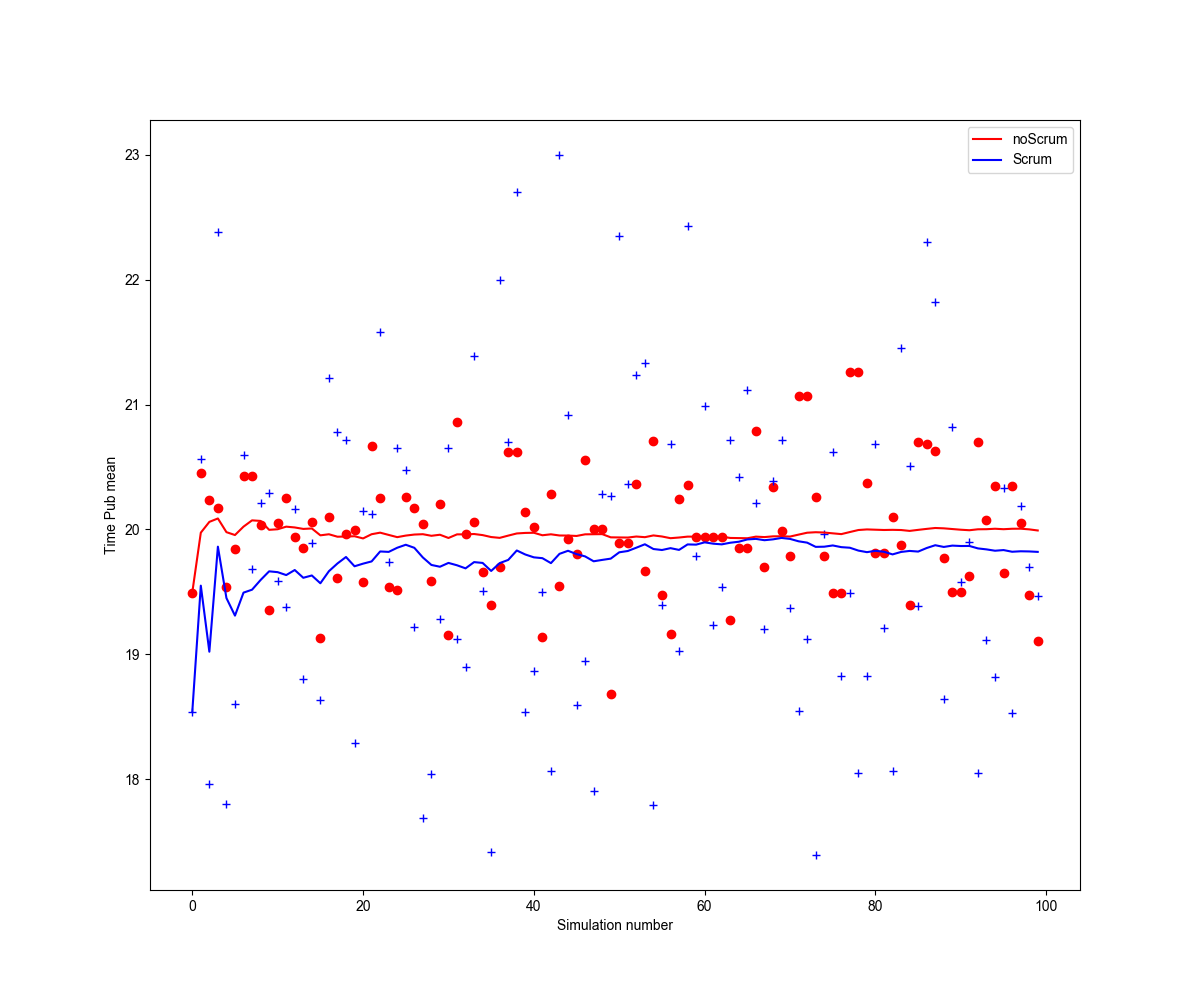
\includegraphics[width=0.8\textwidth]{scrum-img12}
  \label{ex:fig12}
\end{figure}  

\begin{figure}[H]
  \caption{Доля несостоявшихся научных статей в зависимости от номера прогона. Линиями нарисована зависимость скользящего среднего.}
  \centering
    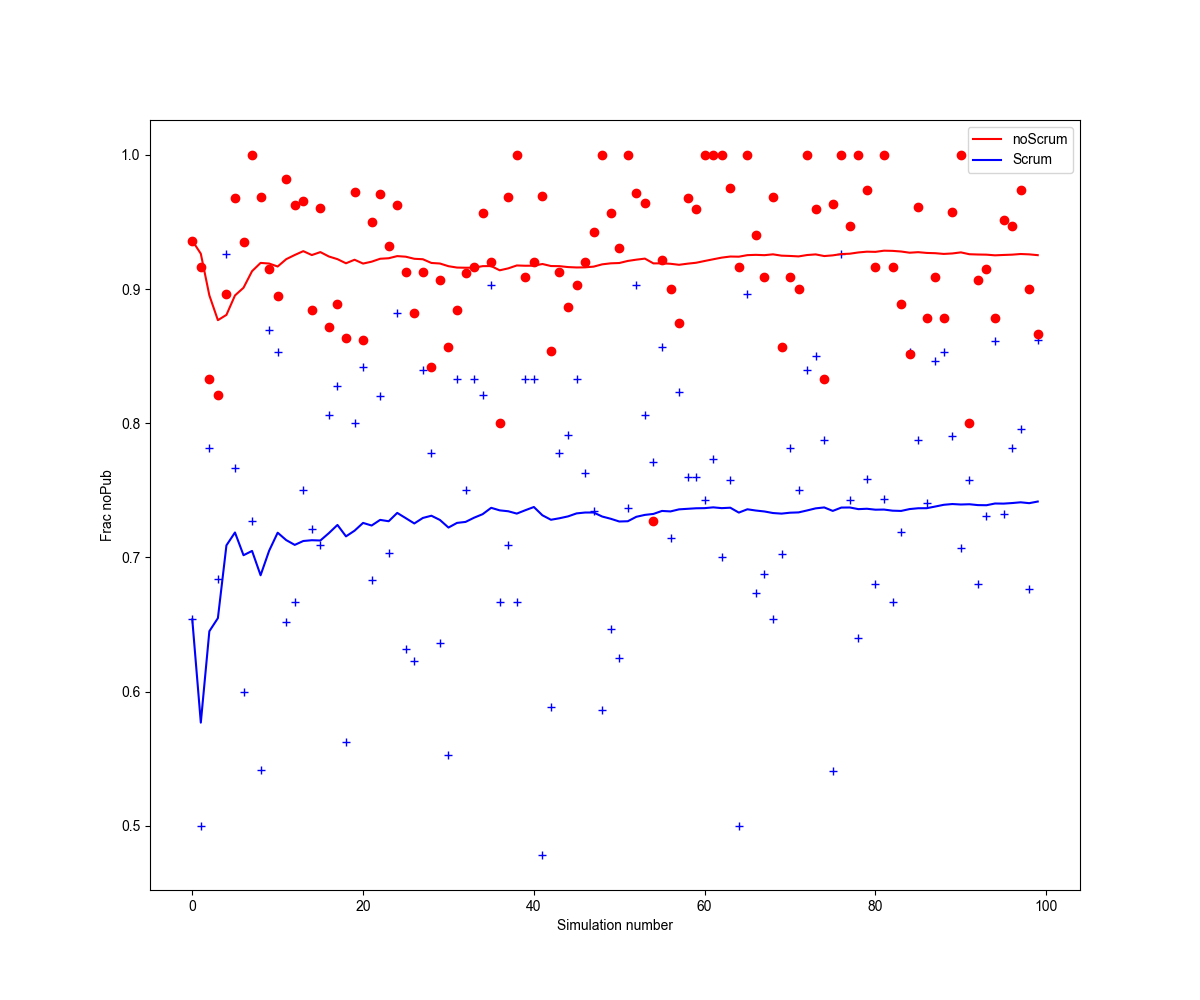
\includegraphics[width=0.8\textwidth]{scrum-img13}
  \label{ex:fig13}
\end{figure}  

Для оценки влияния Scrum на время написания статей $T_{pub}$, автор сравнил время написания статей для двух выборок методом t-теста для сравнения двух независимых выборок.
Результаты показали, что на уровне 1\% значимости длительность написания статей с использованием Scrum не изменяется.

\begin{itemize}
\tightlist
\item
  Среднее время написания научной статьи со Scrum составило 19.90 недель со стандартным отклонением 3.33 недели.
\item
  Среднее время написания научной статьи без Scrum составило 19.90 недель со стандартным отклонением 0.77 недели
\end{itemize}

Автор также дополнительно использовал непараметрический критерий U Манна-Уитни в случае, при котором распределении признаков не соответствует нормальному распределению, результаты которого оказались аналогичны t-тесту.
Полученные результаты свидетельствуют о том, что использование Scrum не ускоряет написание статей, даже при условии того, что функция написания статей не подчиняется нормальному распределению.

Другим показателем, который может быть использован для оценки продуктивности Scrum, является доля \emph{несостоявшихся научных статей}. 
Мы оценили долю \emph{несостоявшихся научных статей} для команд, использующих Scrum и не использующих.

\begin{itemize}
\tightlist
\item
  Доля \emph{несостоявшихся научных статей} в командах, использующих
  Scrum 0.74 со стандартным отклонением 0.02
\item
  Доля \emph{несостоявшихся научных статей} в командах, не использующих
  Scrum составляет 0.92 со стандартным отклонением 0.01
\end{itemize}

Другими словами, из 100\% начатых статей в командах, использующих Scrum, успешными будут 26\% статей. 
В случае, если Scrum не используется, во временные рамки публикационного процесса с требуемым качеством уложатся 8\% статей.

\section{Прогнозирование соавторства}

Коллективное соавторство в написании научных статей имеет детерминированную и случайную структурные составляющие. 
Кроме рациональных аспектов при образовании коллектива соавторов отдельной научной статьи существуют и эмоциональные составляющие. 
Во временной перспективе складываются и распадаются рабочие группы исследователей, обновляется трудовой коллектив и состав подрядчиков, которые участвуют в совместных отраслевых коллаборациях для проведения исследований.

Несмотря на всю сложность соавторства, существуют несколько классов моделей для симуляции образования соавторства. 
В их числе модели на основании случайных графов и модели образования соавторств на основе компетенций соавторов. 
Оба математических аппарата разработаны и применяются в течении нескольких десятков лет по отдельности. 
Но практических применений моделей соавторств в корпоративной практике не так много.

Автор выдвинул гипотезу о том, что необходимо объединить несколько различных типов моделей для того, чтобы лучше понять природу научных коллабораций в отдельной организации. 

Автор данного исследования поставил задачу разработать методику построения модели соавторства для научно-технического центра, учитывающую различные структурные составляющие соавторства. 

В результате автор разработал модель с использованием методов машинного обучения, случайных графов и модели компетенций. 
На основании разработанной модели сделан прогноз развития соавторства в написании научных статей научно-технического центра Газпромнефть.

Практическая ценность результатов данного исследования состоит в следующем: Количественно оценен вклад различных структурных составляющих в формировании соавторств при написании научных статей.

Прогнозирование развития соавторства в написании научных статей позволяет осуществить 
планирование корпоративных ресурсов для поддержания роста научных публикаций.
Понимание кластерной структуры соавторства позволяет производить выравнивание направлений научной деятельности в соответствии со стратегическим планом развития научно-технического центра.


Измерение деятельности научно-исследовательских организаций на основании графа соавторства является хорошо зарекомендовавшей себя практикой. 
Исследователи показывают возможности выявления наиболее производительных авторов (``Highly Productive Authors'') и влиятельных авторов (``Influential Authors''). 

В качестве объекта исследования была выбрана публикационная активность НТЦ Газпромнефть. 
Данные были получены из открытой электронной библиотеки OnePetro международного сообщества нефтегазовых инженеров (SPE). 
После очистки было получено 172 статьи. 
Распределение авторов по годам отображено на рисунке (Рис. \ref{fig:guest2}).

\begin{figure}[H]
  \caption{Распределение авторов по годам.}
  \centering
    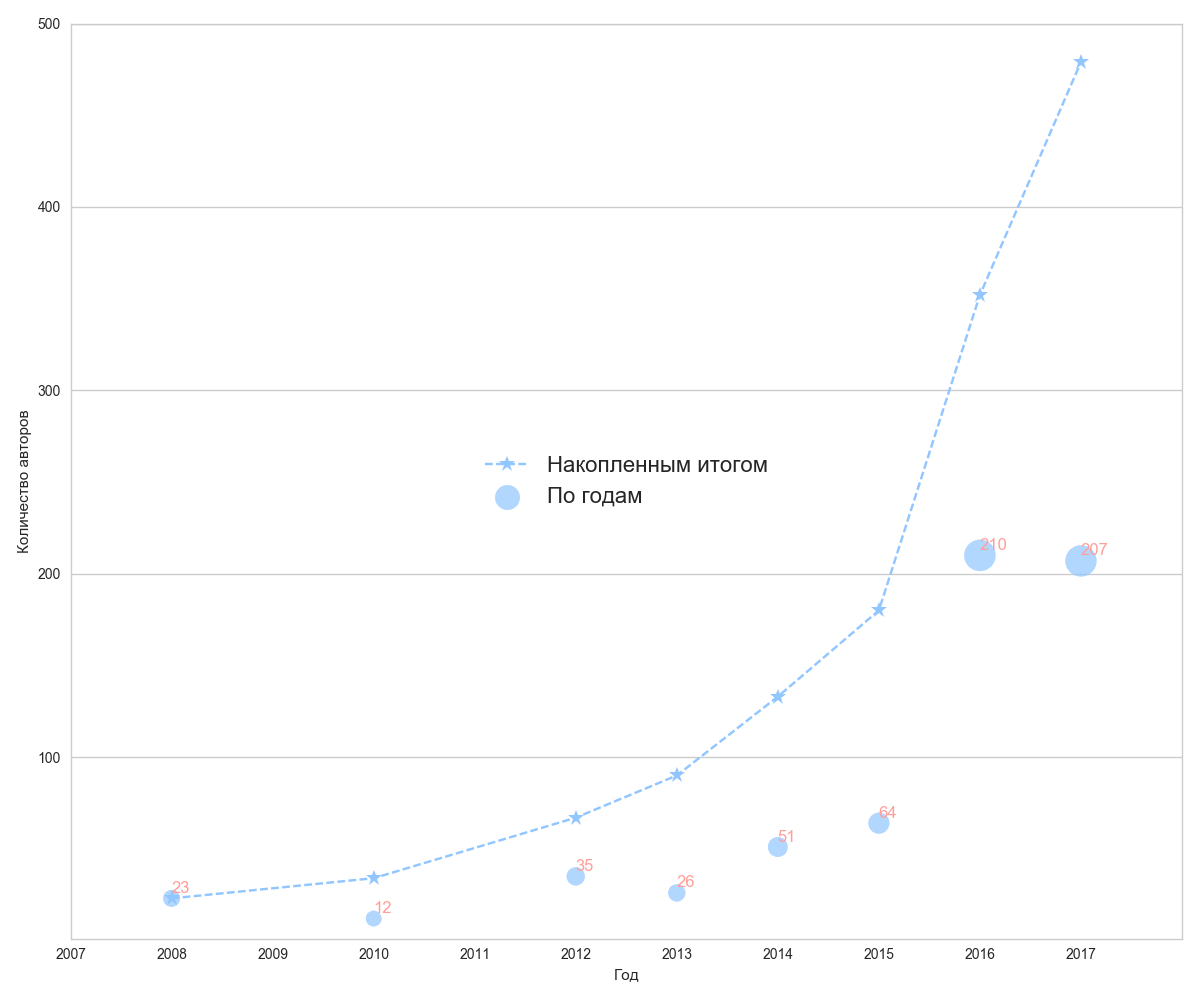
\includegraphics[width=0.8\textwidth]{guest2}
  \label{fig:guest2}
\end{figure}  

Прямолинейным ответом на поставленный исследовательский вопрос может быть интерполяция кривой роста количества авторов.
В результате такой оценки получим  следующую зависимость  $y=13.3816e^0.3422x$ с достоверностью $R^2=0.98$, дающей прогноз 585 авторов в 2018 году. 
Но из графика  \ref{fig:guest2} мы так же видим, что количество авторов в 2017 году (207) меньше чем в 2016 году (210), что может оказаться насыщением роста и повлиять на прогноз.

Построим прогноз на основании графа соавторства. 
Для этого построим двудольный граф соавторства с вершинами: автор (479) и статья (171). 
Авторы обладают техническими компетенциями, статьи характеризуются названием, годом издания и ключевыми словами.

Полученный граф соавторства имеет 26 связанных компонент наибольшая из которых содержит 556 вершин, а остальные – не более 8. 
Малые связанные компоненты относятся к авторам, написавшим свою первую статью. Наличие малых связанных компонент можно рассматривать, как одну из составляющих роста графа соавторств. 
В таблице (Таб. \ref{tab:guest1}) приведены количества и размеры связанных компонент за каждый год нарастающим итогом. 

\begin{table}[H]
\centering
\caption{Размеры связанных компонент графа соавторств по годам нарастающим итогом.}
\label{tab:guest1}
\resizebox{\textwidth}{!}{%
\begin{tabular}{|l|l|l|}
\hline
\textbf{Год} & \textbf{Размеры связанных компонент} & \textbf{Доля малых компонент} \\ \hline
2017 & 556, 8, 8, 8, 6, 5, 5, 5, 4, 4, 4, 4, 4, 4, 3, 3, 3, 2, 2, 2, 2, 2, 2, 2, 2, 2 & 15\% \\ \hline
2016 & 367, 8, 8, 8, 8, 8, 6, 5, 5, 5, 5, 4, 4, 4, 4, 3, 3, 3, 2, 2, 2, 2, 2, 2, 2, 2 & 23\% \\ \hline
2015 & 89, 22, 21, 15, 12, 12, 8, 8, 8, 8, 6, 6, 5, 4, 3, 3, 2, 2, 2, 2, 2 & 63\% \\ \hline
2014 & 46, 18, 15, 12, 12, 10, 8, 8, 8, 7, 6, 5, 4, 4, 3, 2, 2, 2, 2, 2 & 74\% \\ \hline
2013 & 23, 15, 12, 11, 10, 8, 8, 7, 5, 4, 4, 4, 2, 2, 2 & 80\% \\ \hline
2012 & 15, 14, 12, 11, 8, 8, 7, 4, 4, 4 & 83\% \\ \hline
2010 & 12, 9, 8, 8, 4, 3 & 73\% \\ \hline
2008 & 12, 8, 7, 3 & 60\% \\ \hline
\end{tabular}%
}
\end{table}

Таким образом мы видим, что граф соавторства прогрессирует в сегменте малых связанных компонент по количеству и вместе с тем граф становится более связанным – увеличивается количество узлов в главной связанной компоненте. Для уточнения прогнозирования целесообразно будет учесть такое строение. 
На Рис. \ref{fig:guest3} приведена инкрементальная динамика прироста графа соавторства по годам. Уточним, что граф соавторств 2017 года является суммой всех изображенных на (Рис. \ref{fig:guest3}).

\begin{figure}[H]
  \caption{Динамика прироста развития графа соавторств по годам.}
  \centering
    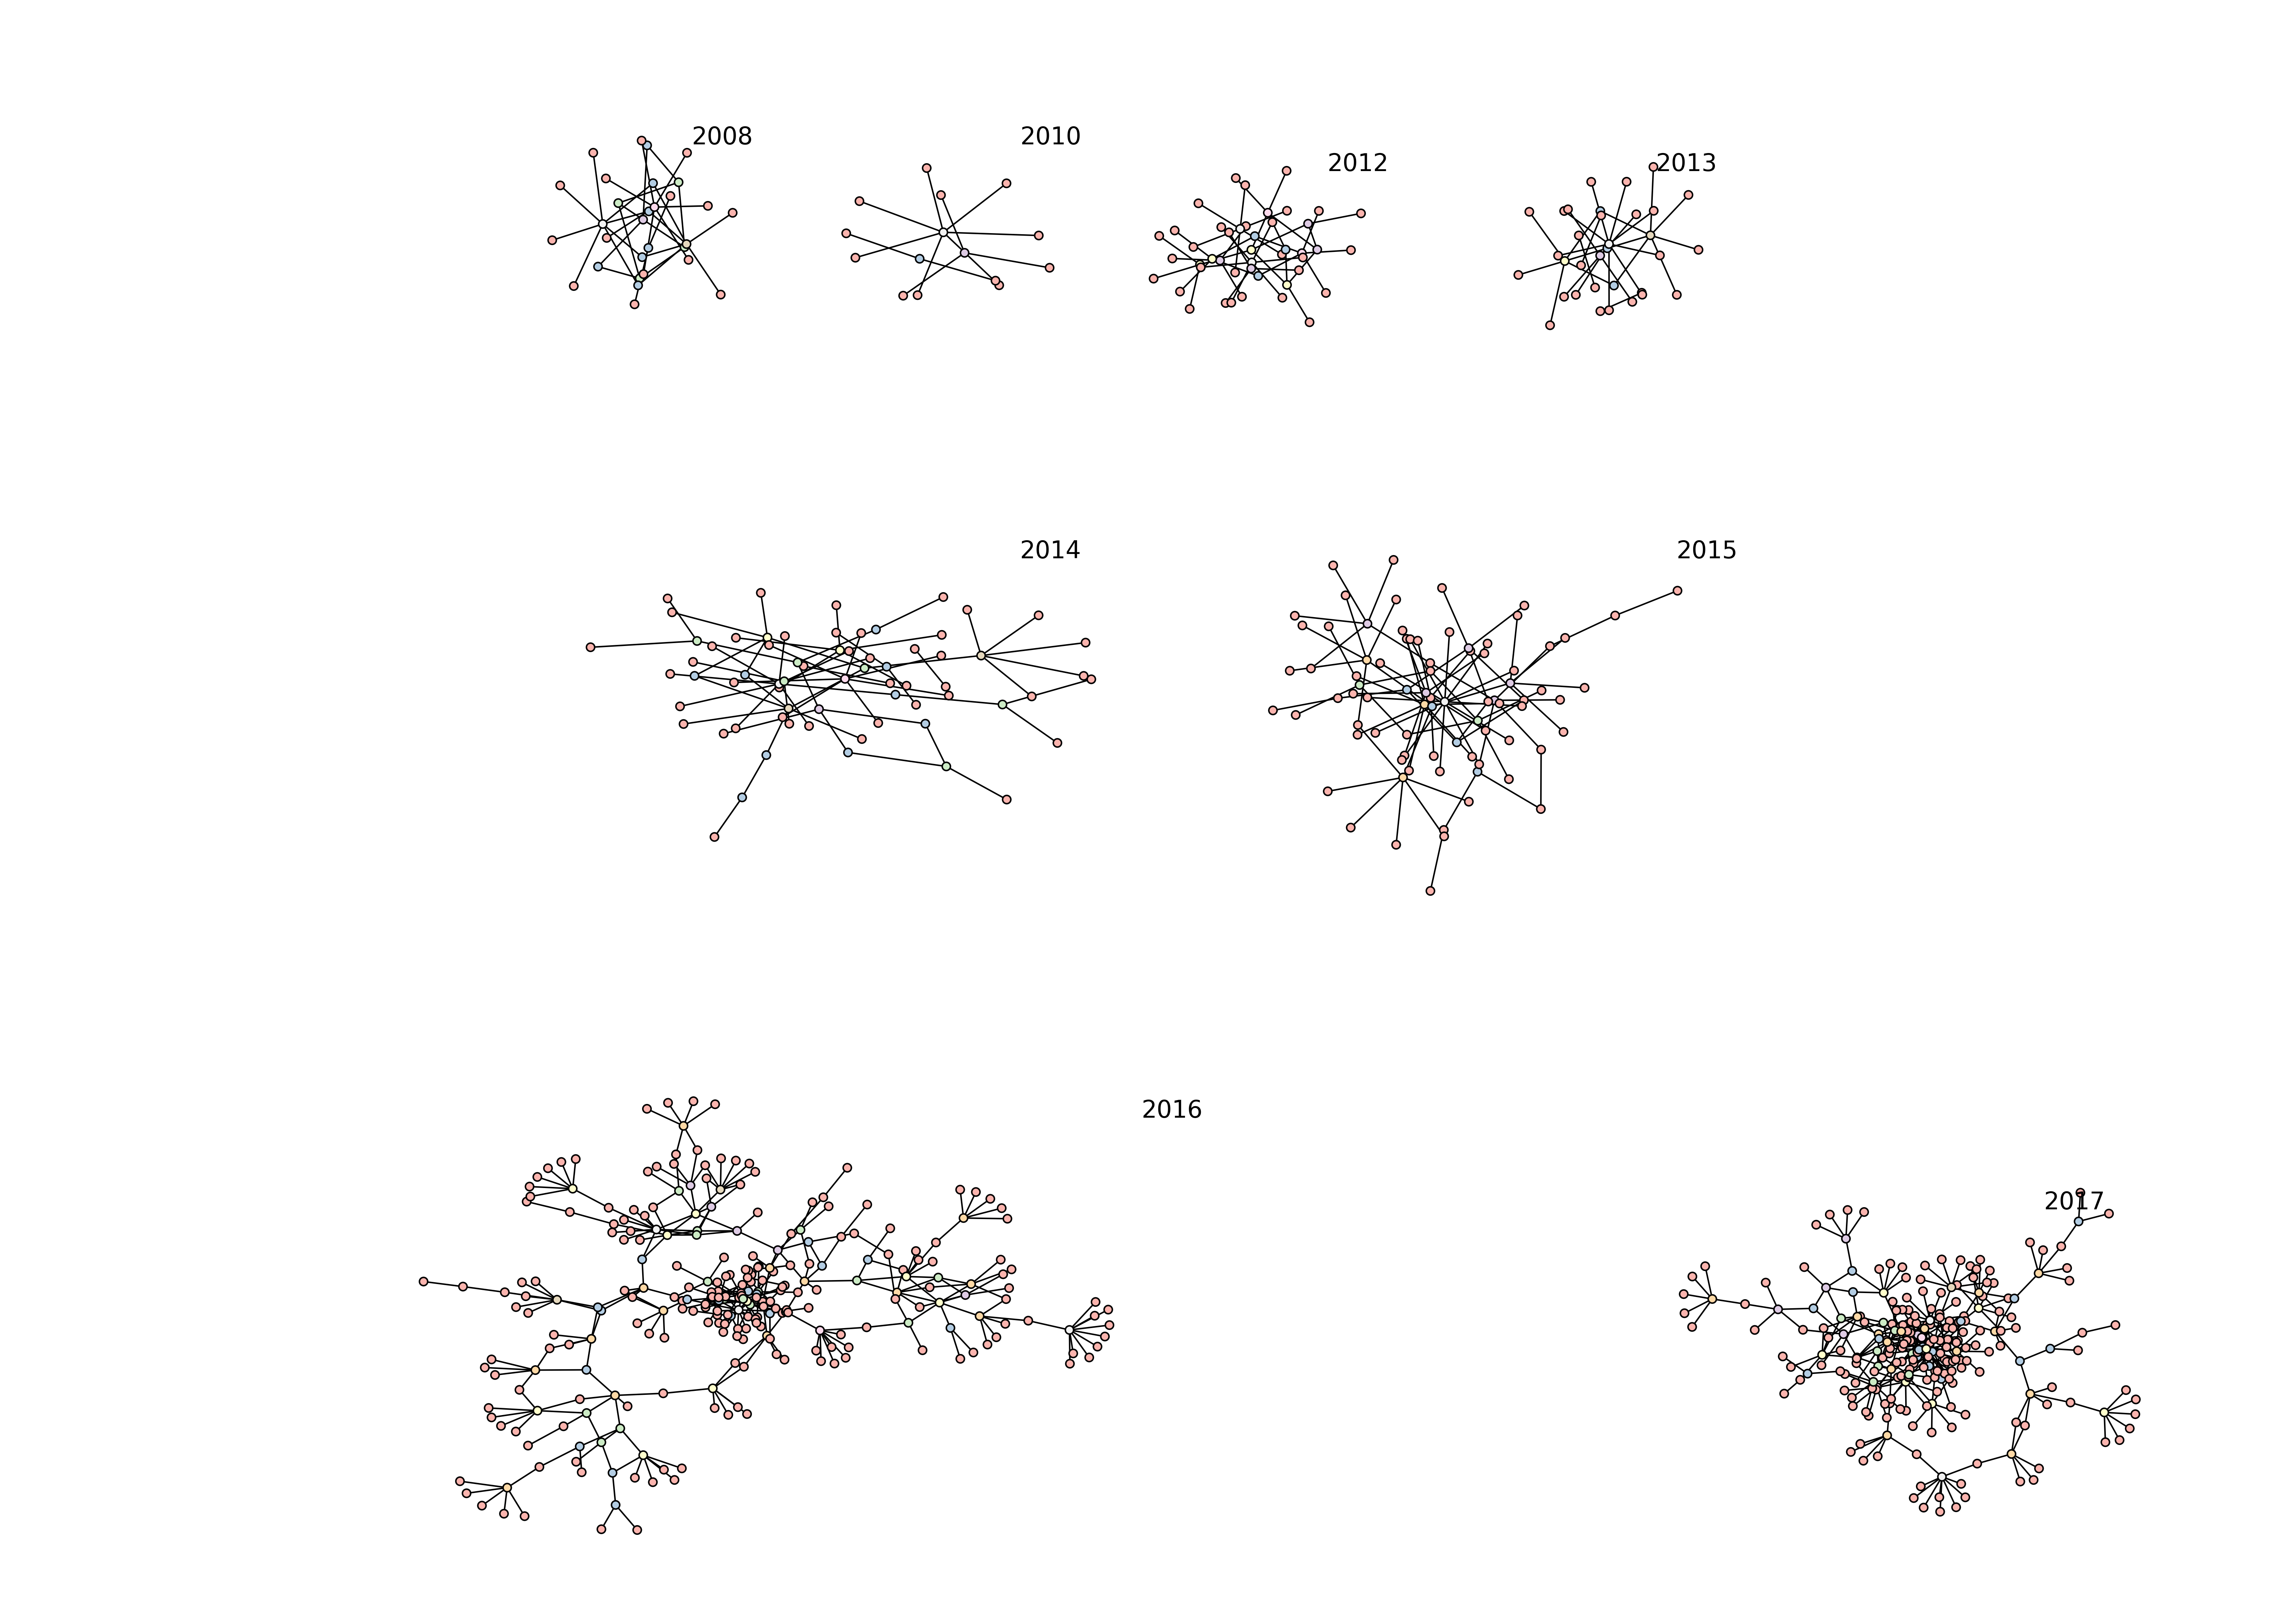
\includegraphics[width=0.99\textwidth]{guest3}
  \label{fig:guest3}
\end{figure}  

Из рисунка (Рис. \ref{fig:guest3}) можно сделать качественной вывод об увеличении ежегодно прибавляемых к графу соавторства связей. Изменение роста ведет к усложнению структуры графа соавторства в 2016 году, что можно констатировать как ``эффект локтя''.Для прогнозирования авторства будем использовать следующие метрики вершин графа:
\begin{itemize}
\tightlist
\item Degree centrality
\item Betweenness centrality
\item Closeness centrality
\item Harmonic centrality
\item Clustering
\end{itemize}

Распределения метрик вершин графа соавторства приведены на рисунке (Рис.\ref{fig:guest4}).

\begin{figure}[H]
  \caption{Метрики вершин графа соавторства.}
  \centering
    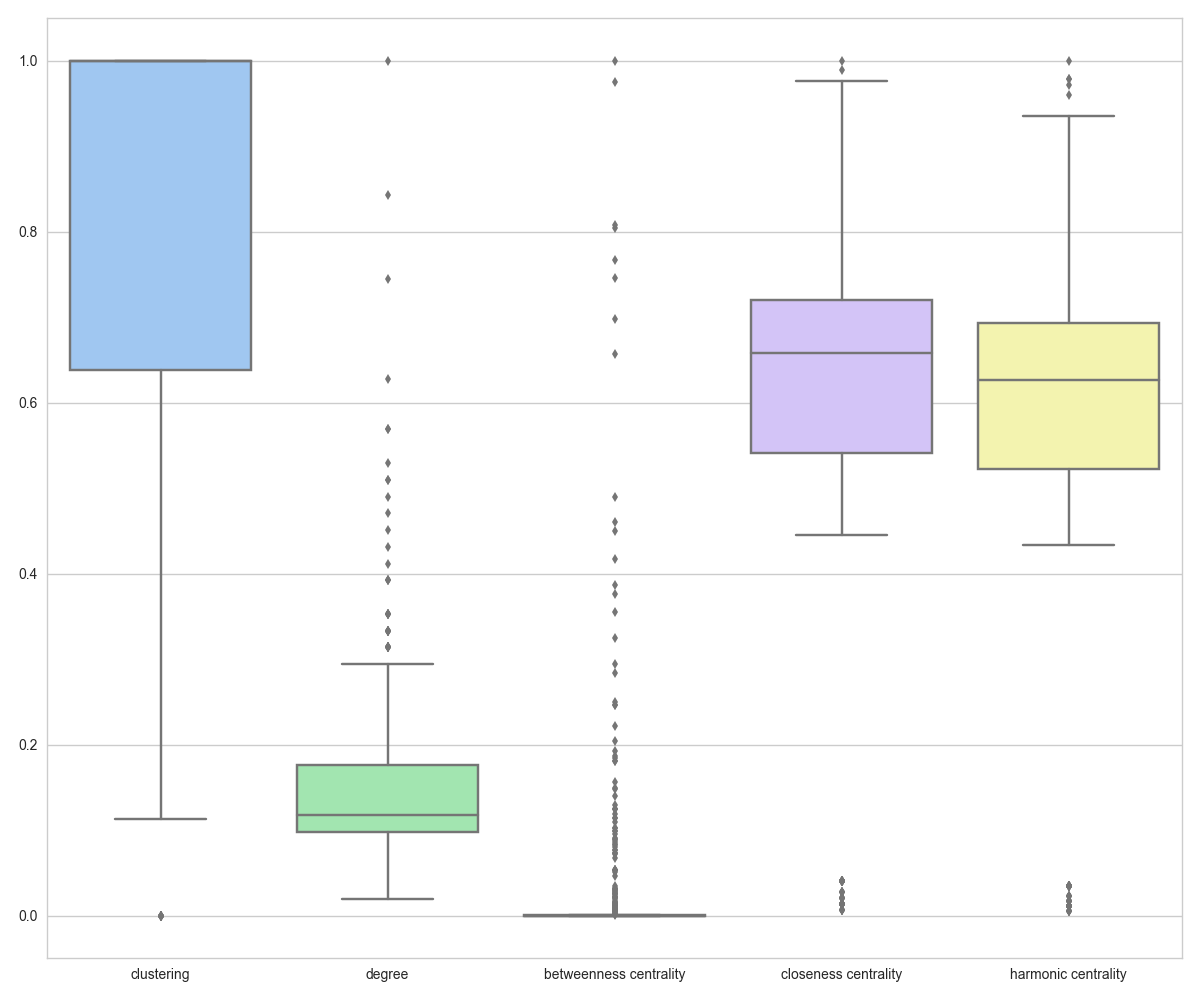
\includegraphics[width=0.8\textwidth]{guest4}
  \label{fig:guest4}
\end{figure}  

Для прогнозирования авторства будем использовать модель бинарной классификации. Выбор модели будем производить на основе ROC-кривой. Обучения модели будем производить на метриках 2016 года. Параметры моделей оптимизированы с помощью кросс-валидации с 5-кратным фолдингом. В результате сравнения различных классификаторов были получены следующие результаты (Таб. \ref{tab:guest2} ).

\begin{table}[H]
\centering
\caption{Сравнение классификаторов по метрике ROC AUC.}
\label{tab:guest2}
\resizebox{\textwidth}{!}{%
\begin{tabular}{|l|l|}
\hline
\textbf{Модель} & \textbf{ROC AUC} \\ \hline
KNeighborsClassifier & 0.66 \\ \hline
RidgeClassifier & 0.73 \\ \hline
RandomForestClassifier & 0.72 \\ \hline
SVM & 0.70 \\ \hline
Multi-layer perceptron & 0.75 \\ \hline
\end{tabular}%
}
\end{table}

Лучшее значение метрики ROC AUC показал классификатор на основе нейронной сети (Multi-layer perceptron) с одним слоем из 10 персептронов. 
Отчет о выполнении прогноза авторства в 2018 году на основе графа соавторства 2017 года приведен в таблице (Таб. \ref{tab:guest3}).

\begin{table}[H]
\centering
\caption{Отчет о выполнении прогноза авторства на 2018 г.}
\label{tab:guest3}
\resizebox{\textwidth}{!}{%
\begin{tabular}{|l|l|l|l|l|}
\hline
 & \textbf{precision} & \textbf{recall} & \textbf{f1-score} & \textbf{support} \\ \hline
\textbf{not author} & 0.80 & 0.98 & 0.88 & 66 \\ \hline
\textbf{author} & 0.80 & 0.20 & 0.32 & 20 \\ \hline
\textbf{Avg / Total} & 0.80 & 0.80 & 0.75 & 86 \\ \hline
\end{tabular}%
}
\end{table}

В результате прогнозирования определено 406 авторов в 2018 году. Если добавить к этому прогнозу сотрудников, которые напишут свою первую статью в 2018 году, то на основании оценки по динамике роста связанных компонент получим прибавку в 15\%. Итого в 2018 году авторами станут 467 сотрудников.

\subsection{Распределение научных направлений на основе соавторств}
\label{sec:allo}
Планирование научно-технического развития исследовательской организации должно быть увязано с реальным положением дел. Такие факторы, как организационная инертность, диверсификация исследований и увлечение созданием ИТ-продуктов, могут существенно исказить любые стратегии и планы развития. Тем не менее, исполнимость планов является важной характеристикой развития, существенно повышающей мотивацию персонала к достижению результата. Поэтому постановка реально, а не только ``на бумаге'' выполнимых задач, необходима. 

Не может быть достаточно только количественных инструментов оценки выполнения научно-исследовательских работ. Формально-бумажная отчетность по НИР не способна отразить увлеченность и вовлеченность исследователей в работу. В то время как малые формы исследовательских работ, такие как презентация на научно-технической конференции или научная статья в рецензируемом периодическом издании, требуют намного более неформального отношения со стороны исследователей.  Анализ развития научно-технической организации на основе публикационной активности является распространенной практикой. Многие исследования анализируют корпусы текстов научных статей и делают заключения о трендах развития. Текстовые данные обладают высоким уровнем шума и даже современные методы анализа на основании word embedding выдают точные прогнозы только на основании огромных объемов текстов, которые не всегда имеются у небольших организаций. При этом именно небольшие научно-исследовательские организации в наибольшей степени страдают от неточности планирования научной деятельности.

Современный фокус применения научных подходов к управленческим решениям приобретает все большую актуальность. С увеличением объемов данных традиционные аналитические средства руководителей организаций становятся все менее эффективными. С другой стороны, необходимого объема данных для устойчивой работы современных алгоритмов часто бывает недостаточно. В авангарде этой тенденции возникает задача адаптации и создания новых эвристик для таких классических задач, как кластеризация для применения в организационной среде.

Кластеризация данных на основании статической модели получила развитие с открытием таких алгоритмов, как PAM, CLARANS, DBSCAN, CURE и ROCK. Тем не менее, в последнее время особое внимание привлечено к алгоритмам кластеризации на основании динамической модели, например, CHAMELEON. Основная идея алгоритма CHAMELEON заключается в использовании метрик близости графа, построенного на основании набора кластеризуемых данных с помощью метода ``k наиболее близких соседей'' (KNN). Метрики графа оказываются более эффективными для разбиения данных ``сверху вниз'' в случае сложных объектов.

Разнообразие алгоритмов кластеризации не умаляет важность задачи оценки их качества. Но в условиях ограниченного количества данных и для обеспечения управленческих решений качество кластеризации должно иметь не только математически обоснованную, но и уверенную наглядную составляющую. Другими словами, чтобы ``с одного взгляда было понятно'' и не нужно было вникать в формулы. Таковы требования современного бизнеса.

С формальной точки зрения необходимо решить задачу обучения без учителя (unsupervised machine learning) для графа соавторств, отнести кластеры к определенным тематикам и выявить изменения в кластерах со временем.
Кластеризация графа соавторства может быть осуществлена на основании различных метрик вершин: 
\begin{itemize}
\tightlist
\item Degree centrality
\item Betweenness centrality
\item Closeness centrality
\item Harmonic centrality
\item Clustering
\end{itemize}

Рассмотрим содержательный смысл метрики Betweenness centrality применительно к задаче кластеризации графа соавторств научно-технической организации. Метрика Betweenness centrality характеризует то, насколько данный узел важен для связанности графа. Связи в графе соавторств отражают совместную исследовательскую работу. Графы соавторств не всегда являются связанными, обычно это несколько связанных компонент разного размера. 

Связанные компоненты являются естественными кластерами. Небольшие связанные компоненты отражают начальные инициативы – это первые статьи сотрудников. Но главная связанная компонента может содержать 90\% вершин графа соавторства и нуждается в отдельном подходе к кластеризации. 

Для выделения кластеров из главной связанной компоненты графа соавторств возможно использовать методику искусственного удаления вершин с наибольшей метрикой Betweenness centrality. При каждом таком удалении вершины граф может распадаться на несколько несвязанных компонент. На рисунке (Рис.\ref{fig:allo2}) приведена модель такого разделения.

\begin{figure}[H]
  \caption{Модель разделения графа. а.Связанный изначальный граф. б.Тот же граф, но после удаления вершины с наибольшей метрикой Betweenness centrality уже представляет две связанных компоненты.}
  \centering
    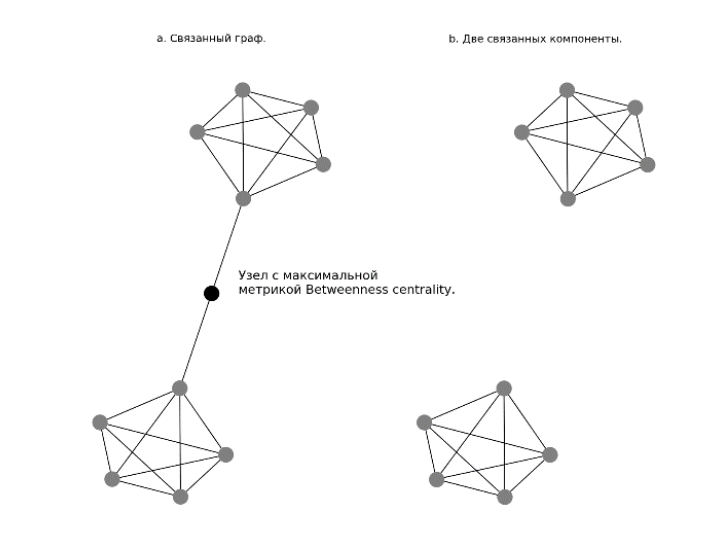
\includegraphics[width=0.8\textwidth]{allo2}
  \label{fig:allo2}
\end{figure}  

Каждую из получившихся при таком распаде связанных компонент можно анализировать на однородность тематики на основании текстов статей, которыми она образована. В результате нескольких итераций мы получим набор кластеров.
Предложенный автором метод является эвристическим и нуждается в проверке по определенному формальному критерию. Для задач кластеризации таким критерием принято считать метрики близости объектов в кластере и расстояния между объектами в разных кластерах.

Сходимость данного метода обеспечивается путем поиска минимума функционала ошибок определения кластеров:

\begin{equation}
\vert WSS - BSS \vert \rightarrow min , 
\label{eq:allo1}
\end{equation}
где $WSS$ - это функция связанности кластера $C_i$:

\begin{equation}
WSS = \sum_i \sum_{x \in C_i} ( x - m_i)^2 , 
\label{eq:allo2}
\end{equation}
а $BSS$ это функция разделения кластеров $C_i$:

\begin{equation}
BSS = \sum_i \vert C_i \vert ( m - m_i)^2 , 
\label{eq:allo3}
\end{equation}
где $\vert C_i \vert $ - это размер кластера $C_i$.

Междисциплинарные исследования приводят к тому, что статьи будут относится к нескольким тематикам, так что полученные кластера будут пересекающимися – не эксклюзивными. Таккая кластеризания называется"мягкой".

В качестве объекта исследования была выбрана публикационная активность НТЦ ``Газпромнефть''. Данные были получены из открытой электронной библиотеки OnePetro международного сообщества нефтегазовых инженеров (SPE). После очистки было получено 172 статьи.
Построим прогноз на основании графа соавторства. Для этого построим двудольный граф соавторства с вершинами: автор (479) и статья (171). Авторы обладают техническими компетенциями, статьи характеризуются названием, годом издания и ключевыми словами.
Полученный граф соавторства имеет 26 связанных компонент наибольшая из которых содержит 556 вершин, а остальные не более 8. Связанные компоненты с количеством узлов до 8 являются считать первыми статьями сотрудников.
Рассмотрим наибольшую связанную компоненту (556 вершин). Выделим подграф из основного графа соавторства на основании узлов, относящихся к наибольшей связанной компоненте. Получившийся подграф отображен на рисунке (Рис. \ref{fig:allo3}).

\begin{figure}[H]
  \caption{Подграф наибольшей связанной компоненты графа соавторства.}
  \centering
    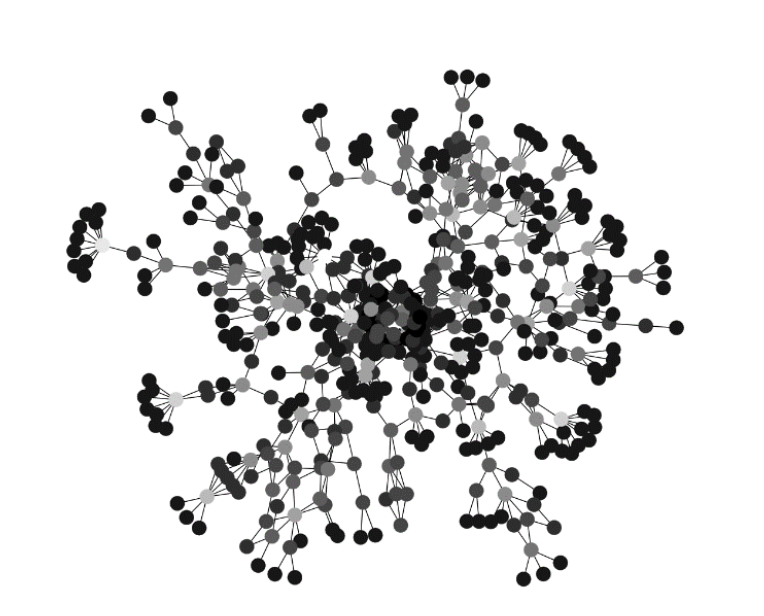
\includegraphics[width=0.8\textwidth]{allo3}
  \label{fig:allo3}
\end{figure}  

Рассчитаем для полученного подграфа метрику Betweenness centrality. Полученные значения Betweenness centrality отображены на рисунке (Рис. \ref{fig:allo4}). Нулевые значения Betweenness centrality не отображены.

\begin{figure}[H]
  \caption{Гистограмма значений Betweenness centrality для подграфа наибольшей связанной компоненты графа соавторств.}
  \centering
    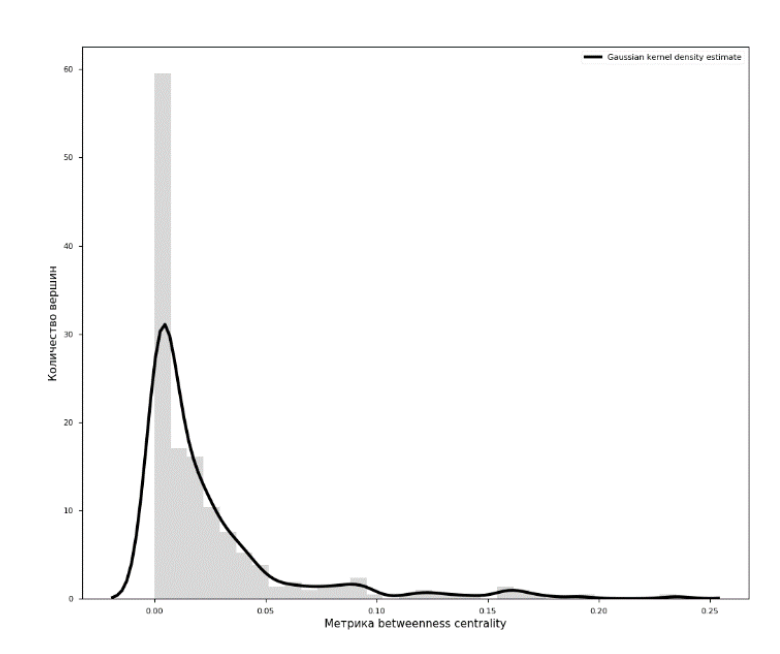
\includegraphics[width=0.8\textwidth]{allo4}
  \label{fig:allo4}
\end{figure}  

Как мы видим из Рис. \ref{fig:allo4} значения метрики Betweenness centrality в третьем квартиле принадлежат всего 23 вершинам, что составляет менее 5 \% от всего количества вершин.
Применим алгоритм искусственного удаления вершин с наибольшим значением метрики Betweenness centrality. На рисунке (Рис. \ref{fig:allo5}) отображена зависимость количества связанных компонент от количества искусственно удаленных вершин

\begin{figure}[H]
  \caption{Зависимость количества связанных компонент от количества искусственно удаленных вершин.}
  \centering
    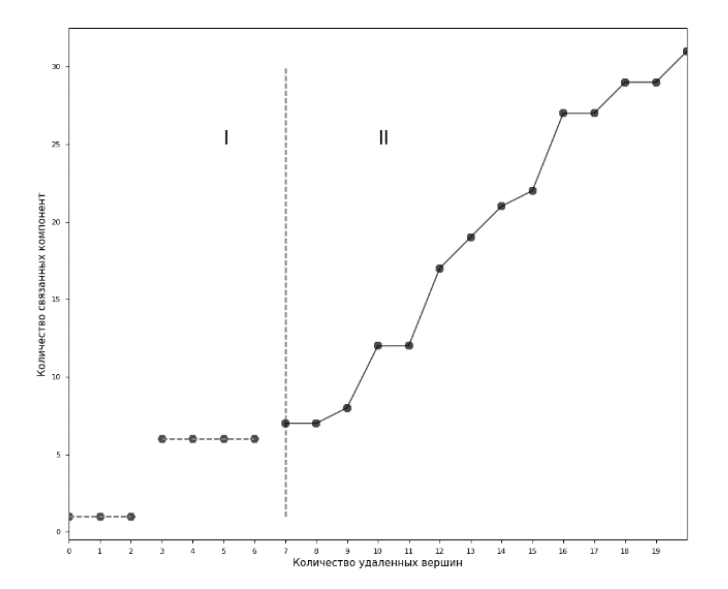
\includegraphics[width=0.8\textwidth]{allo5}
  \label{fig:allo5}
\end{figure}  

При удалении вершин поведение графа происходит в двух режимах:

\begin{enumerate}[I/]
\item Удержание связанности
\item Экспоненциальный распад
\end{enumerate}

Отличительной чертой режима I является то, что граф остается связанным при удалении вершин с высокими значениями метрики Betweenness centrality. Это означает, что удаляемые вершины не являются единственными связующими между кластерами.
Отличительной особенностью режима II является следование степенной модели распада графа, когда удаление каждого узла вызывает степенной рост появления новых связанных компонент.
Рассмотрим более подробно вторую половину режима I алгоритма, когда граф разделился на 6 связанных компонент. Размеры этих компонент составляют 511, 34, 1, 1, 1, 1. И среди них ярко выраженное направление исследований по Теме 1 представлено именно компонентой с 34 узлами, представленной на рисунке (Рис. \ref{fig:allo6}).

\begin{figure}[H]
  \caption{Кластер исследователей по Теме 1, выделенный в результате применения метода удаления вершин в наибольшим значением метрики Betweenness centrality.}
  \centering
    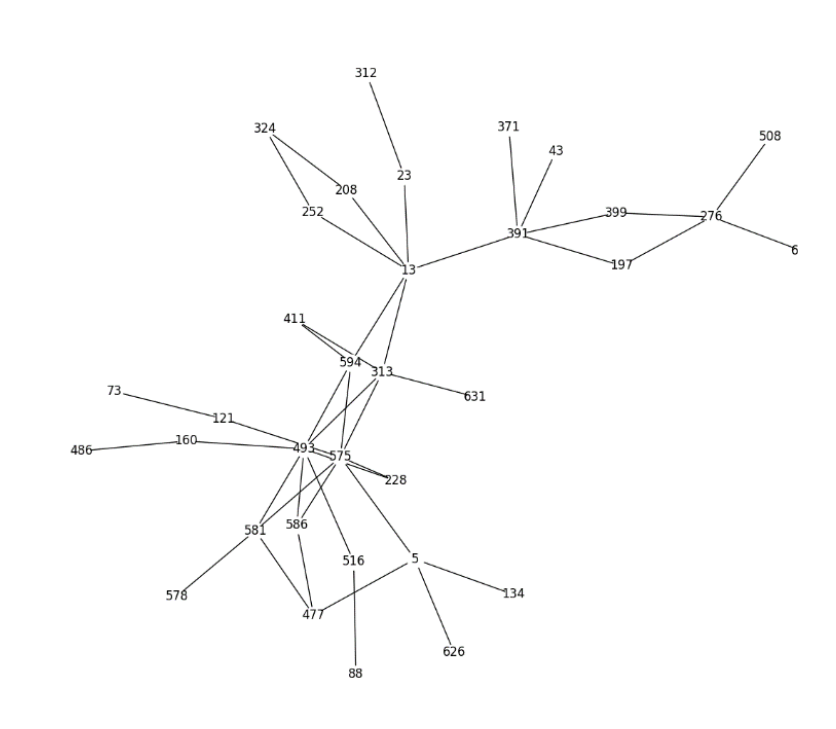
\includegraphics[width=0.8\textwidth]{allo6}
  \label{fig:allo6}
\end{figure}  

Мы рассмотрели выделение одного кластера подробно. Полный алгоритм выделения кластеров будет состоять из следующих шагов:
\begin{enumerate}
\tightlist
\item Построение двудольного графа соавторств: $G$
\item Определение метрики Betweenness centrality для графа $G$
\item Определение вершины с максимальной метрикой $N_{max(Betweenness centrality)}$
\item Удаление вершины $N_{max(Betweenness centrality)}$ из графа $G$
\item Получение списка связанных компонент графа $G$
\item Вычисление метрики качества полученных кластеров $BSS$ и $WSS$
\item Далее алгоритм повторяется для каждой связанной компоненты
\item Алгоритм завершается, когда все связанные компоненты представляют кластеры удовлетворительного качества.
\end{enumerate}

Для выбранного графа соавторства были выделены 16 кластеров.
Для вычисления значений  и W на основании текстов статей было использовано векторное представление текста статьи (VSM). Каждая статья представлена в виде вектора со значениями метрики BM25 для каждого слова. Статьи рассматривались как ``мешок слов'' (bag of words). Для измерения дистанции между векторными представлениями статей была использована косинусная мера.
На рисунке (Рис. \ref{fig:allo7}) изображена матрица раздельности кластеров .

\begin{figure}[H]
  \caption{Матрица раздельности кластеров. По осям отображены номера кластеров. В ячейках значения функции $BSS$.}
  \centering
    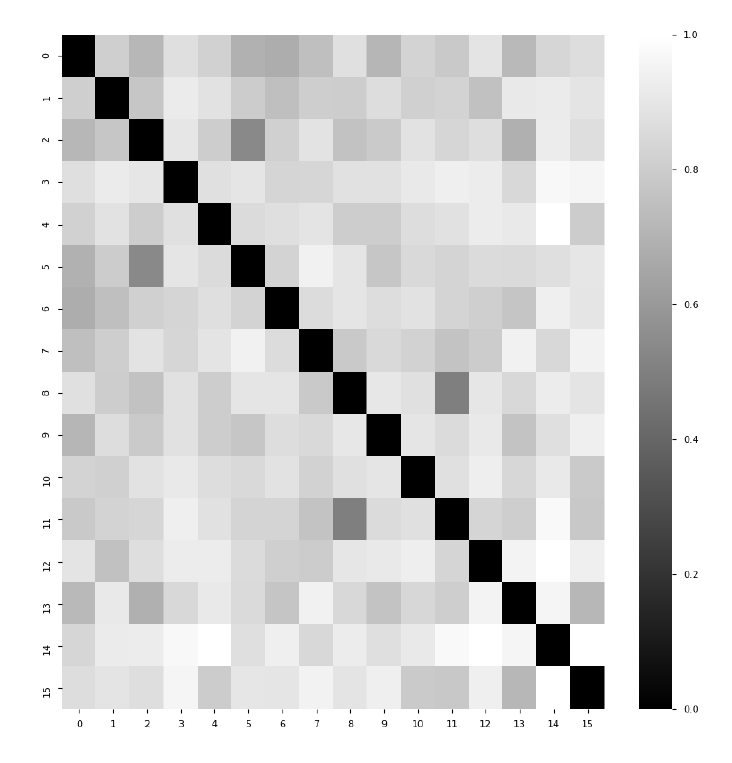
\includegraphics[width=0.8\textwidth]{allo7}
  \label{fig:allo7}
\end{figure}  

Для сравнения полученной кластеризации статей была проведена кластеризация с помощью алгоритма KMeans, показавшая схожие результаты (Рис. \ref{fig:allo8}).

\begin{figure}[H]
  \caption{Сравнение предлагаемого в статье алгоритма кластеризации и алгоритма KMeans.}
  \centering
    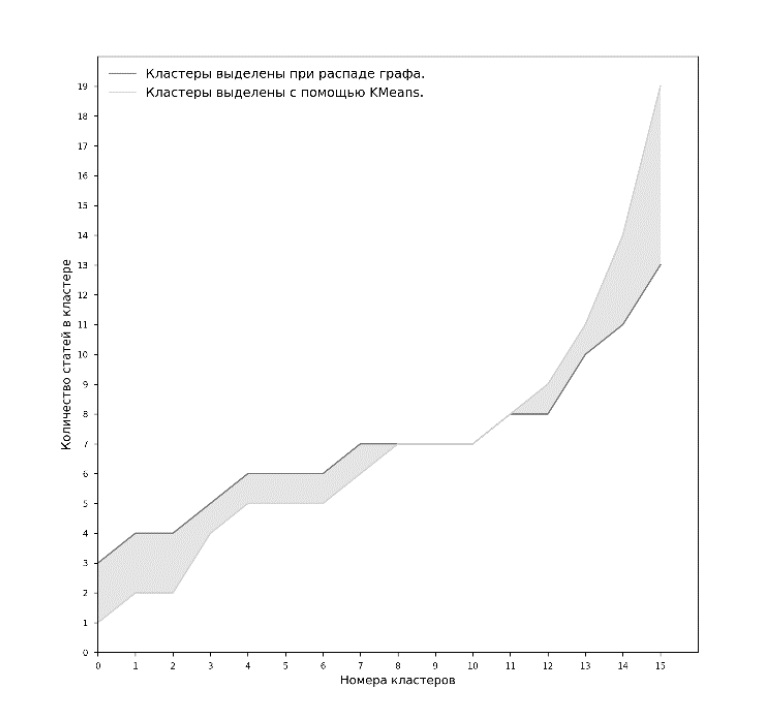
\includegraphics[width=0.8\textwidth]{allo8}
  \label{fig:allo8}
\end{figure}  

С помощью KMeans была произведена кластеризация статьей, а затем из графа соавторства были определены кластеры авторов на основании полученных кластеров статей.

\section[Вероятностная модель текста]{Вероятностная модель скрытых тем на основе архива журнала ``Нефтяное Хозяйство''}

Вопрос о том, по какому пути движется прикладная наука и технологии, является ключевым для любой научно-технической области. 
Традиционно определение векторов развития производилось и производится экспертами по предметному направлению, однако значительный рост объемов информации и увеличение числа направлений развития свидетельствуют о необходимости доработки и совершенствования этого инструментария и выработке дополнительных методов исследования индустриальных трендов. 
В данном исследовании автором проанализированы тренды нефтяной индустрии посредством автоматизированной обработки текстов научных статей в отраслевом журнале ``Нефтяное хозяйство''. 
Выявляя наиболее часто встречаемые темы в журнале за период с 2008 по 2016 годы, мы сделали вывод об увеличении значимости трудноизвлекаемых запасов и росте интереса к методам разработки подобных месторождений. 

Журнал ``Нефтяное хозяйство'' посвящен нефтегазовой проблематике.
В нем публикуются статьи, посвященные широкому кругу вопросов нефтегазового сектора: экономических, технических, технологических, экологических и информационных. Издание насчитывает почти вековую историю и выходит каждый месяц с 1920 года. 
Все публикуемые статьи проходят процедуру рецензирования.
Журнал включен в Российский индекс научного цитирования (РИНЦ) и международную систему индексирования Scopus. 
Материалы журнала находятся в закрытом доступе и распространяются по подписке. 
Основные рубрики журнала: 

\begin{itemize}
\tightlist
\item новости нефтегазовых компаний;
\item нефтяная и газовая промышленность;
\item экономика, управление, право;
\item геология и геологоразведочные работы;
\item бурение;
\item разработка и эксплуатация нефтяных месторождений;
\item проектирование и обустройство месторождений;
\item техника и технологии добычи нефти;
\item нефтепромысловое оборудование;
\item транспорт и подготовка нефти;
\item экологическая и промышленная безопасность;
\item информационные технологии. 
\end{itemize}

Как видно, журнал подробно рассматривает практически все аспекты функционирования нефтяных компаний – от экономико-правовых вопросов, до технологических аспектов и тонкостей.

Для проведения исследования редакцией были любезно предоставлены архивы статей журнала ``Нефтяное хозяйство'' за период 2008-2016 гг. 
В выборке содержится 108 выпусков журналов, со статьями от 3517 авторов. 
В каждом из выпусков журналов содержатся все статьи номера, таким образом, была получена сплошная выборка, в которой содержались материалы по самым различным содержательным направлениям. 
В среднем, в номере журнала ``Нефтяного хозяйства'' около 20-25 статей. 
Были рассмотрены именно выпуски журнала, так как они являлись единицей анализа. 
Авторами статей журнала являются научные сотрудники, инженеры и отраслевые эксперты, многие из них кандидаты и доктора наук. 

Процесс исследования имел следующие этапы:

\begin{enumerate}
\item 
Изначально архивы представлены в виде файлов в формате PDF. 
Иногда это был единый файл (биндер) со статьями за весь год, а иногда разрозненные файлы с отдельными статьями. 
В обоих случаях файлы были предназначены для печати, то есть содержали оглавления, номера страниц, тематические вставки и другие редакторские элементы. 
Для анализа нужны были только тексты в виде предложений поэтому автором был реализован программный модуль для приведения всех данных к такому формату. 
Отметим, что, исходя из выбранной методики, важно было сохранить порядок слов и разделение на предложения, при этом необходимо было сохранять принадлежность к выпуску, а не к статье, так как минимальной единицей временного анализа выбран один выпуск.

\item 
На втором этапе анализа происходило приведение слов к основным формам. 
Для анализа и сравнения слов методами частотного и вероятностного анализа необходимо сузить возможные варианты употребления словоформ. 
Существуют несколько алгоритмов для решения этой задачи (нормализации текста), в данном случае был использована стемминг. 
Стеммингом называют процедуру нахождения основы слова, при этом основа и корень слова могут различаться между собой.  
Одним из наиболее распространенных инструментов является стеммер Портера, который, однако, часто обрезает слово больше необходимого, что затрудняет получение правильной основы слова, например, кровать->крова. 
Также стеммер Портера не справляется со всевозможными изменениями корня слова (например, выпадающие и беглые гласные), характерными для русского языка. 
Поэтому автор остановился на использовании технологии стемминга компании ``Яндекс'' - MyStem. 
Данная программа производит морфологический анализ текста на русском языке. 
Она умеет строить гипотетические разборы для слов, не входящих в словарь и предлагает несколько вариантов основ слова. 
Тем не менее, автор сочел необходимым поддерживать обратный словарь для полученных словоформ, чтобы сохранять связь между изначальным словом и полученной словоформой. Отдельной веткой обработки подвергались аббревиатуры, широко распространенные в нефтегазовой отрасли. 
Определение аббревиатур производилось на основе словаря аббревиатур, созданного и поддерживаемого в компании ГазпромНефть в рамках проекта Корпоративной Википедии \cite{khasanov2016corporate}.

\item 
На третьем этапе исследования проводилось формирование словаря. 
Известно, что наибольшую смысловую нагрузку несут не одиночные слова, а сочетания слов, в частности пары слов – биграммы. 
Для выделения биграммов автором был использован эвристические алгоритмы. 
Была составлена матрица биграммов в окрестности 5 слов для каждого из предложений. 
Затем были рассчитаны частоты использования каждого из биграммов, после чего были зафиксированы 5\% наиболее встречаемых словосочетаний.

\item 
На четвертом этапе словари отдельных слов и биграммов были объединены для общей обработки алгоритмами выделения тематик. 
Получившийся словарь был проанализирован, на предмет выделения высоко- и низкочастотных слов для их фильтрации. 
Традиционно окончательное формирование словаря производится с помощью стоп-слов. 
Алгоритмы выделения стоп-слов не использовались автором в данной статье. 
Это решение было обусловлено тем, что добавление словаря стоп-слов не добавляло точности и вносило субъективный характер исследования.

\item 
На заключительном пятом этапе производилось построение модели тематик. 
Для этого был использован инструмент BigARTM \cite{ianina2017multi}. 
На этом этапе были получены матрицы распределение тем для документа ($\Theta$) и распределение слов для темы ($\Phi$). 
Для повышения точности алгоритма автором был применен аналитический подход, уточняющий регуляризационные параметры на основании метрик. 
\end{enumerate}

Основной метрикой для выявления факта сходимости модели тем является метрика Perplexity. 
График зависимости Perplexity от количества проходов по корпусу текстов отображен на (Рис. \ref{fig:nx1}).
\begin{figure}[H]
  \caption{Зависимость метрики Perplexity от количества проходов по корпусу текстов.}
  \centering
    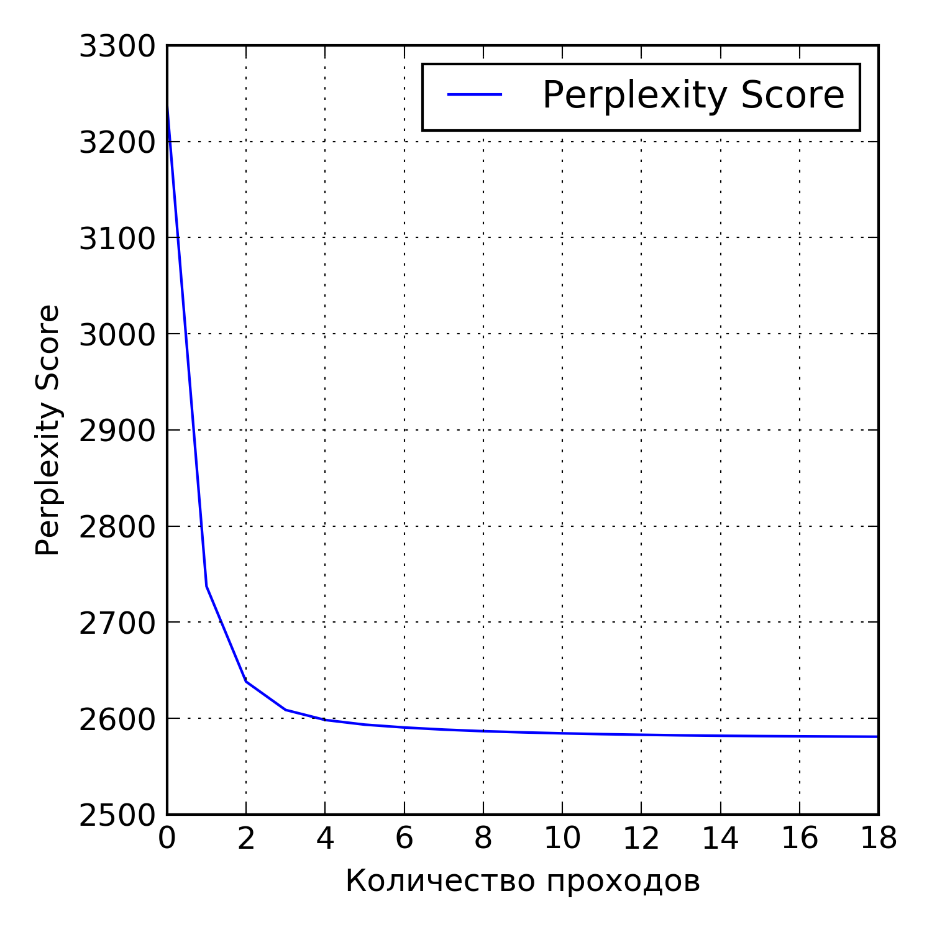
\includegraphics[width=0.8\textwidth]{nx1}
  \label{fig:nx1}
\end{figure}  

Из (Рис. \ref{fig:nx1}) видно, что за три прохода модель показала приемлемую сходимость и не нуждается в дальнейшей оптимизации. 

Важными метриками качества модели тем являются степень разрежённости матриц $\Phi$ и $\Theta$. Повлиять на эти метрики можно с помощью параметров $\tau$, соответствующих регуляризаторов. На рисунках Рис. \ref{fig:nx2}  и Рис. \ref{fig:nx3} отображены зависимости для разрежённости матриц  $\Phi$ и $\Theta$.

\begin{figure}[H]
  \caption{Зависимость разрежённости матрицы $\Theta$ от параметра регуляризации $\tau$.}
  \centering
    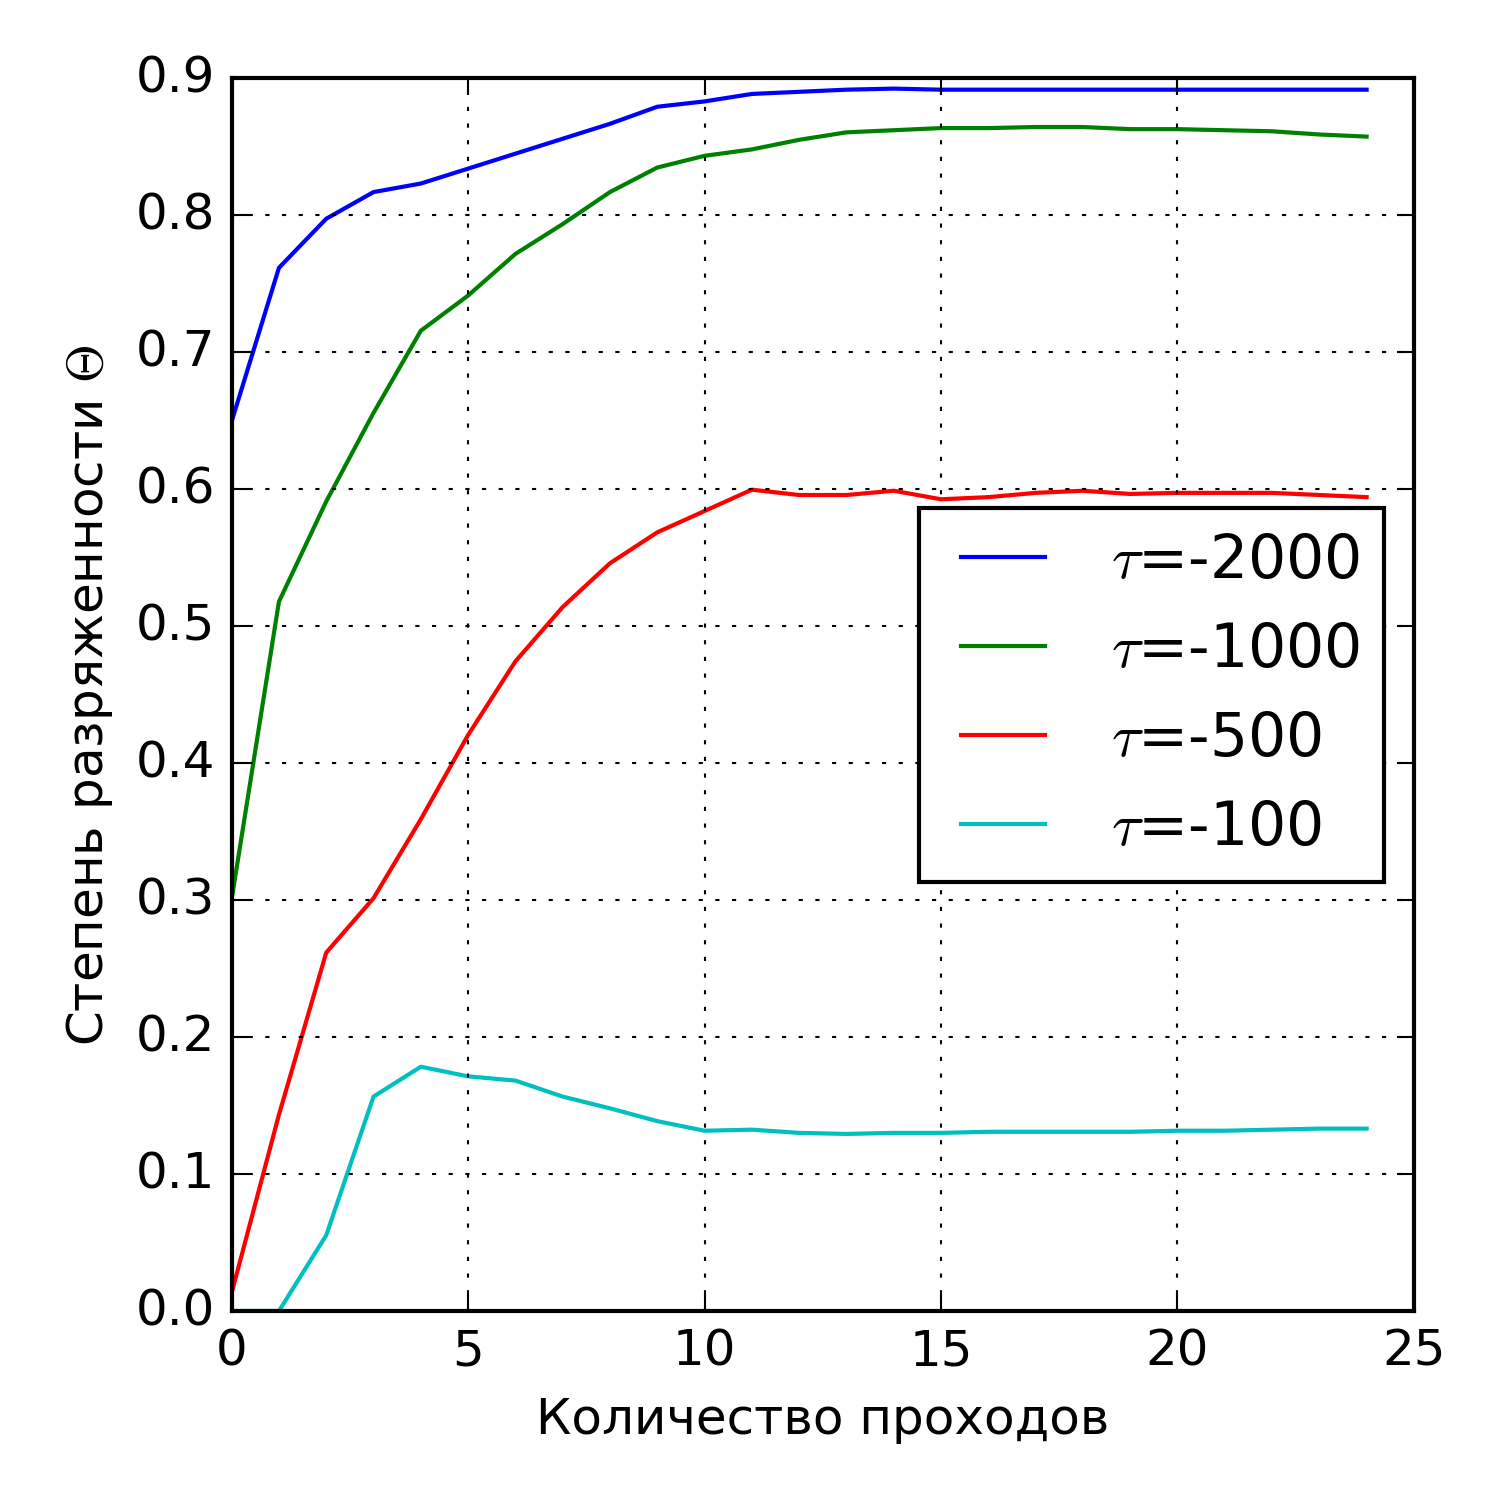
\includegraphics[width=0.8\textwidth]{nx2}
  \label{fig:nx2}
\end{figure}  

\begin{figure}[H]
  \caption{Зависимость разрежённости матрицы $\Phi$ от параметра регуляризации $\tau$.}
  \centering
    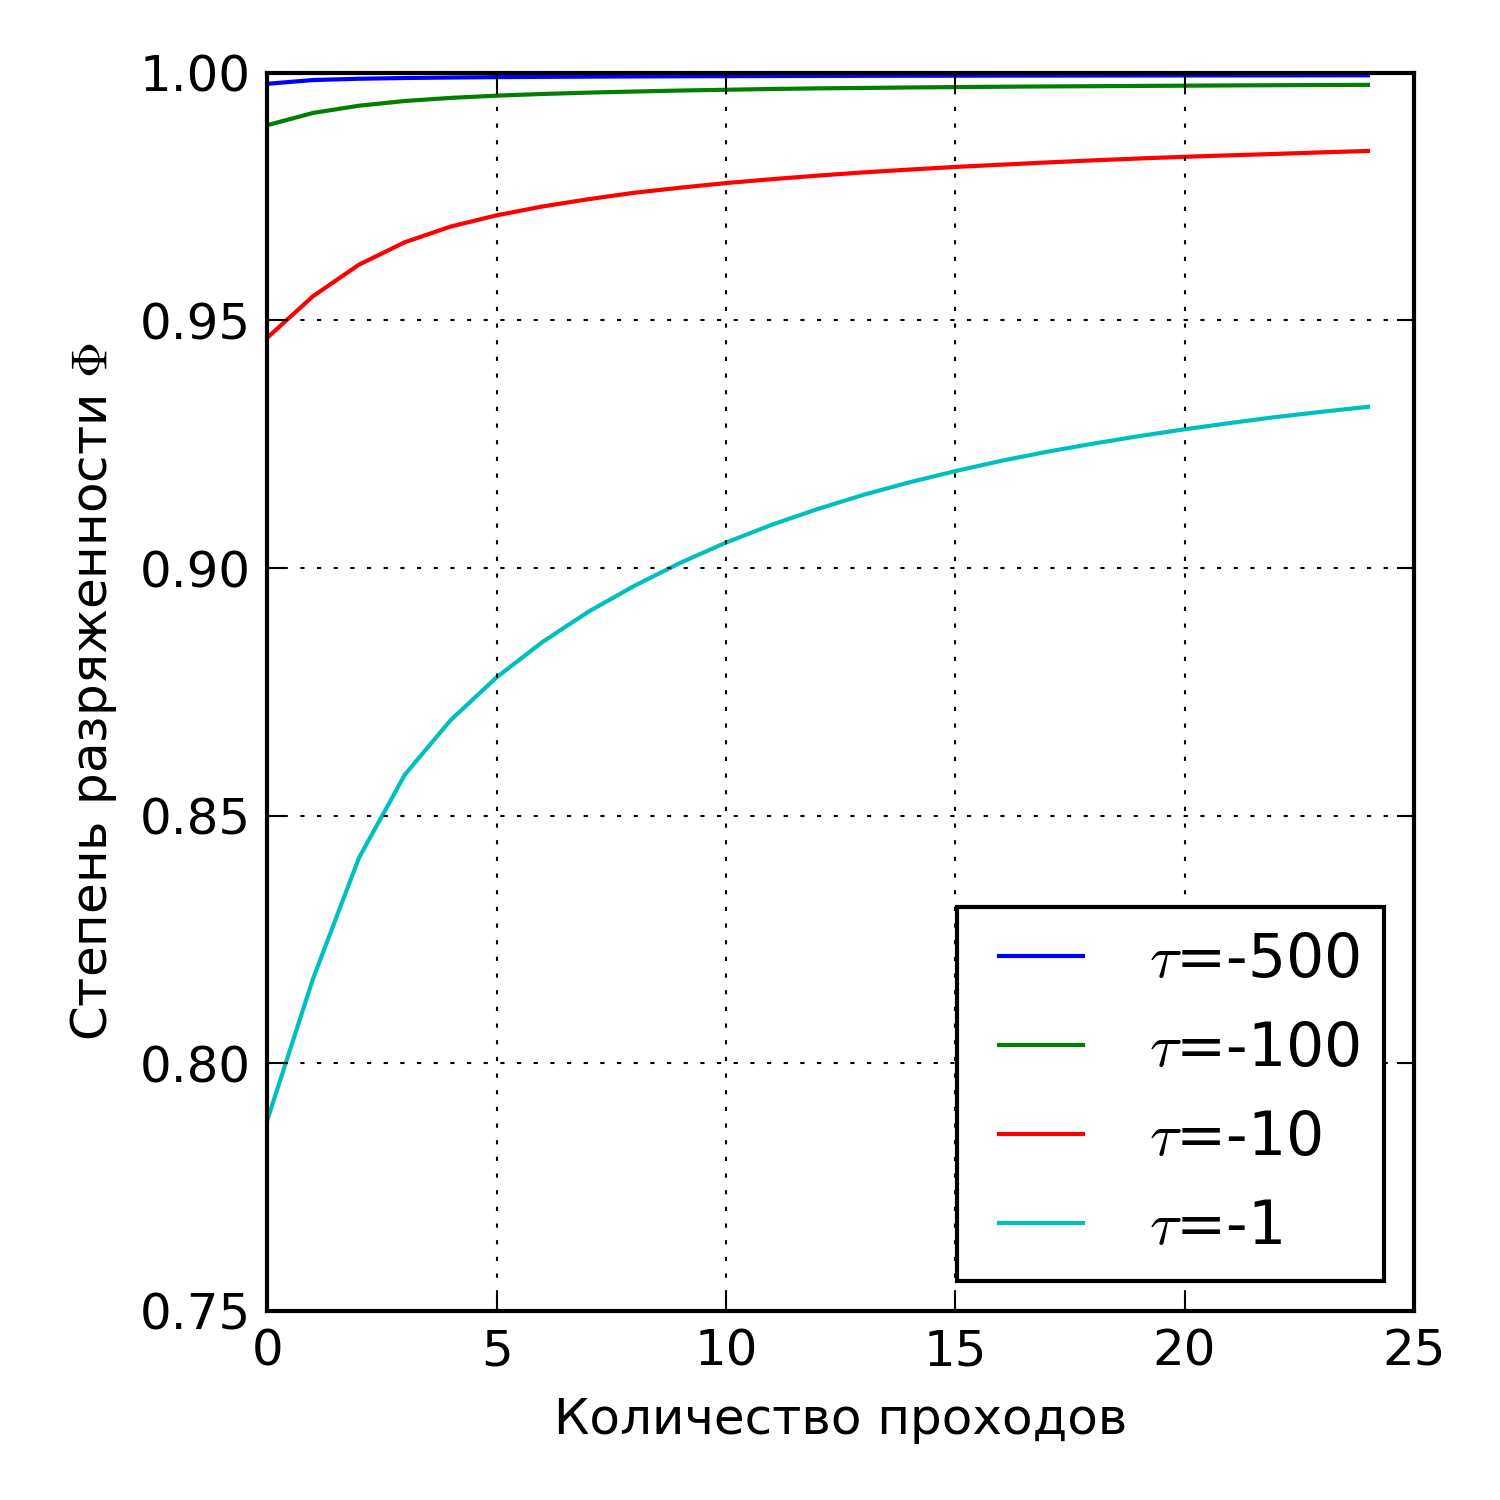
\includegraphics[width=0.8\textwidth]{nx3}
  \label{fig:nx3}
\end{figure}  

На основании зависимостей отображенных на  Рис. \ref{fig:nx2}  и Рис. \ref{fig:nx3} автором были выбраны параметры регуляризации модели тем, позволяющие достичь оптимального соотношения между значимыми терминами и шумовыми.

Тематическая модель, полученная в результате данного исследования, может быть представлена в различных формах. Уровень шумовых терминов мешает интерпретировать результаты, поэтому от запланированных 12 тем содержательных осталось шесть. В Таблице (Таб. \ref{tab:nx1}) представлены темы выделенные с помощью модели. 

\begin{table}[H]
\centering
\caption{Фрагмент матрицы $\Phi$ для терминов  с максимальными вероятностями.}
\label{tab:nx1}
\resizebox{\textwidth}{!}{%
\begin{tabular}{|l|l|l|l|l|l|}
\hline
\textbf{Тема1} & \textbf{Тема2} & \textbf{Тема3} & \textbf{Тема4} & \textbf{Тема5} & \textbf{Тема6} \\ \hline
электронный & ЭЦН & сдвиг & почва & нефтегазоносность & ингибитор \\ \hline
знание & УЭЦН & сигнал & добавка & свод & разлом \\ \hline
автоматизация & сероводород & окисление & композиция & компания & деформация \\ \hline
интегрировать & фациальный & разрушение & знание & впадина & трещиноватость \\ \hline
пользователь & гамма & деформация & агрегат & сепарация & исследовательский \\ \hline
архив & доломит & реологический & загрязнение & миграция & известняк \\ \hline
хранение & замер & песчаный & ПЗП & прогнозный & порода \\ \hline
доступ & депрессия & осадки & надежность & активность & политехнический \\ \hline
подразделение & агент & капиллярный & камень & филиал & штанга \\ \hline
платформа & каротаж & сечение & окисление & цемент & приемистость \\ \hline
\end{tabular}%
}
\end{table}

Можно с уверенностью сказать, что термины, собранные в столбце $Тема1$ характеризуют тематику управления знаниями. 
В столбце $Тема2$ представлена тема добычи. 
Остальные столбцы тоже могут быть достаточно однозначно проинтерпретированы. 
А для машинной обработки набор терминов важнее чем обобщающая его тема.

\begin{figure}[H]
  \caption{Матрица $\Theta$: Распределение тем для документов.}
  \centering
    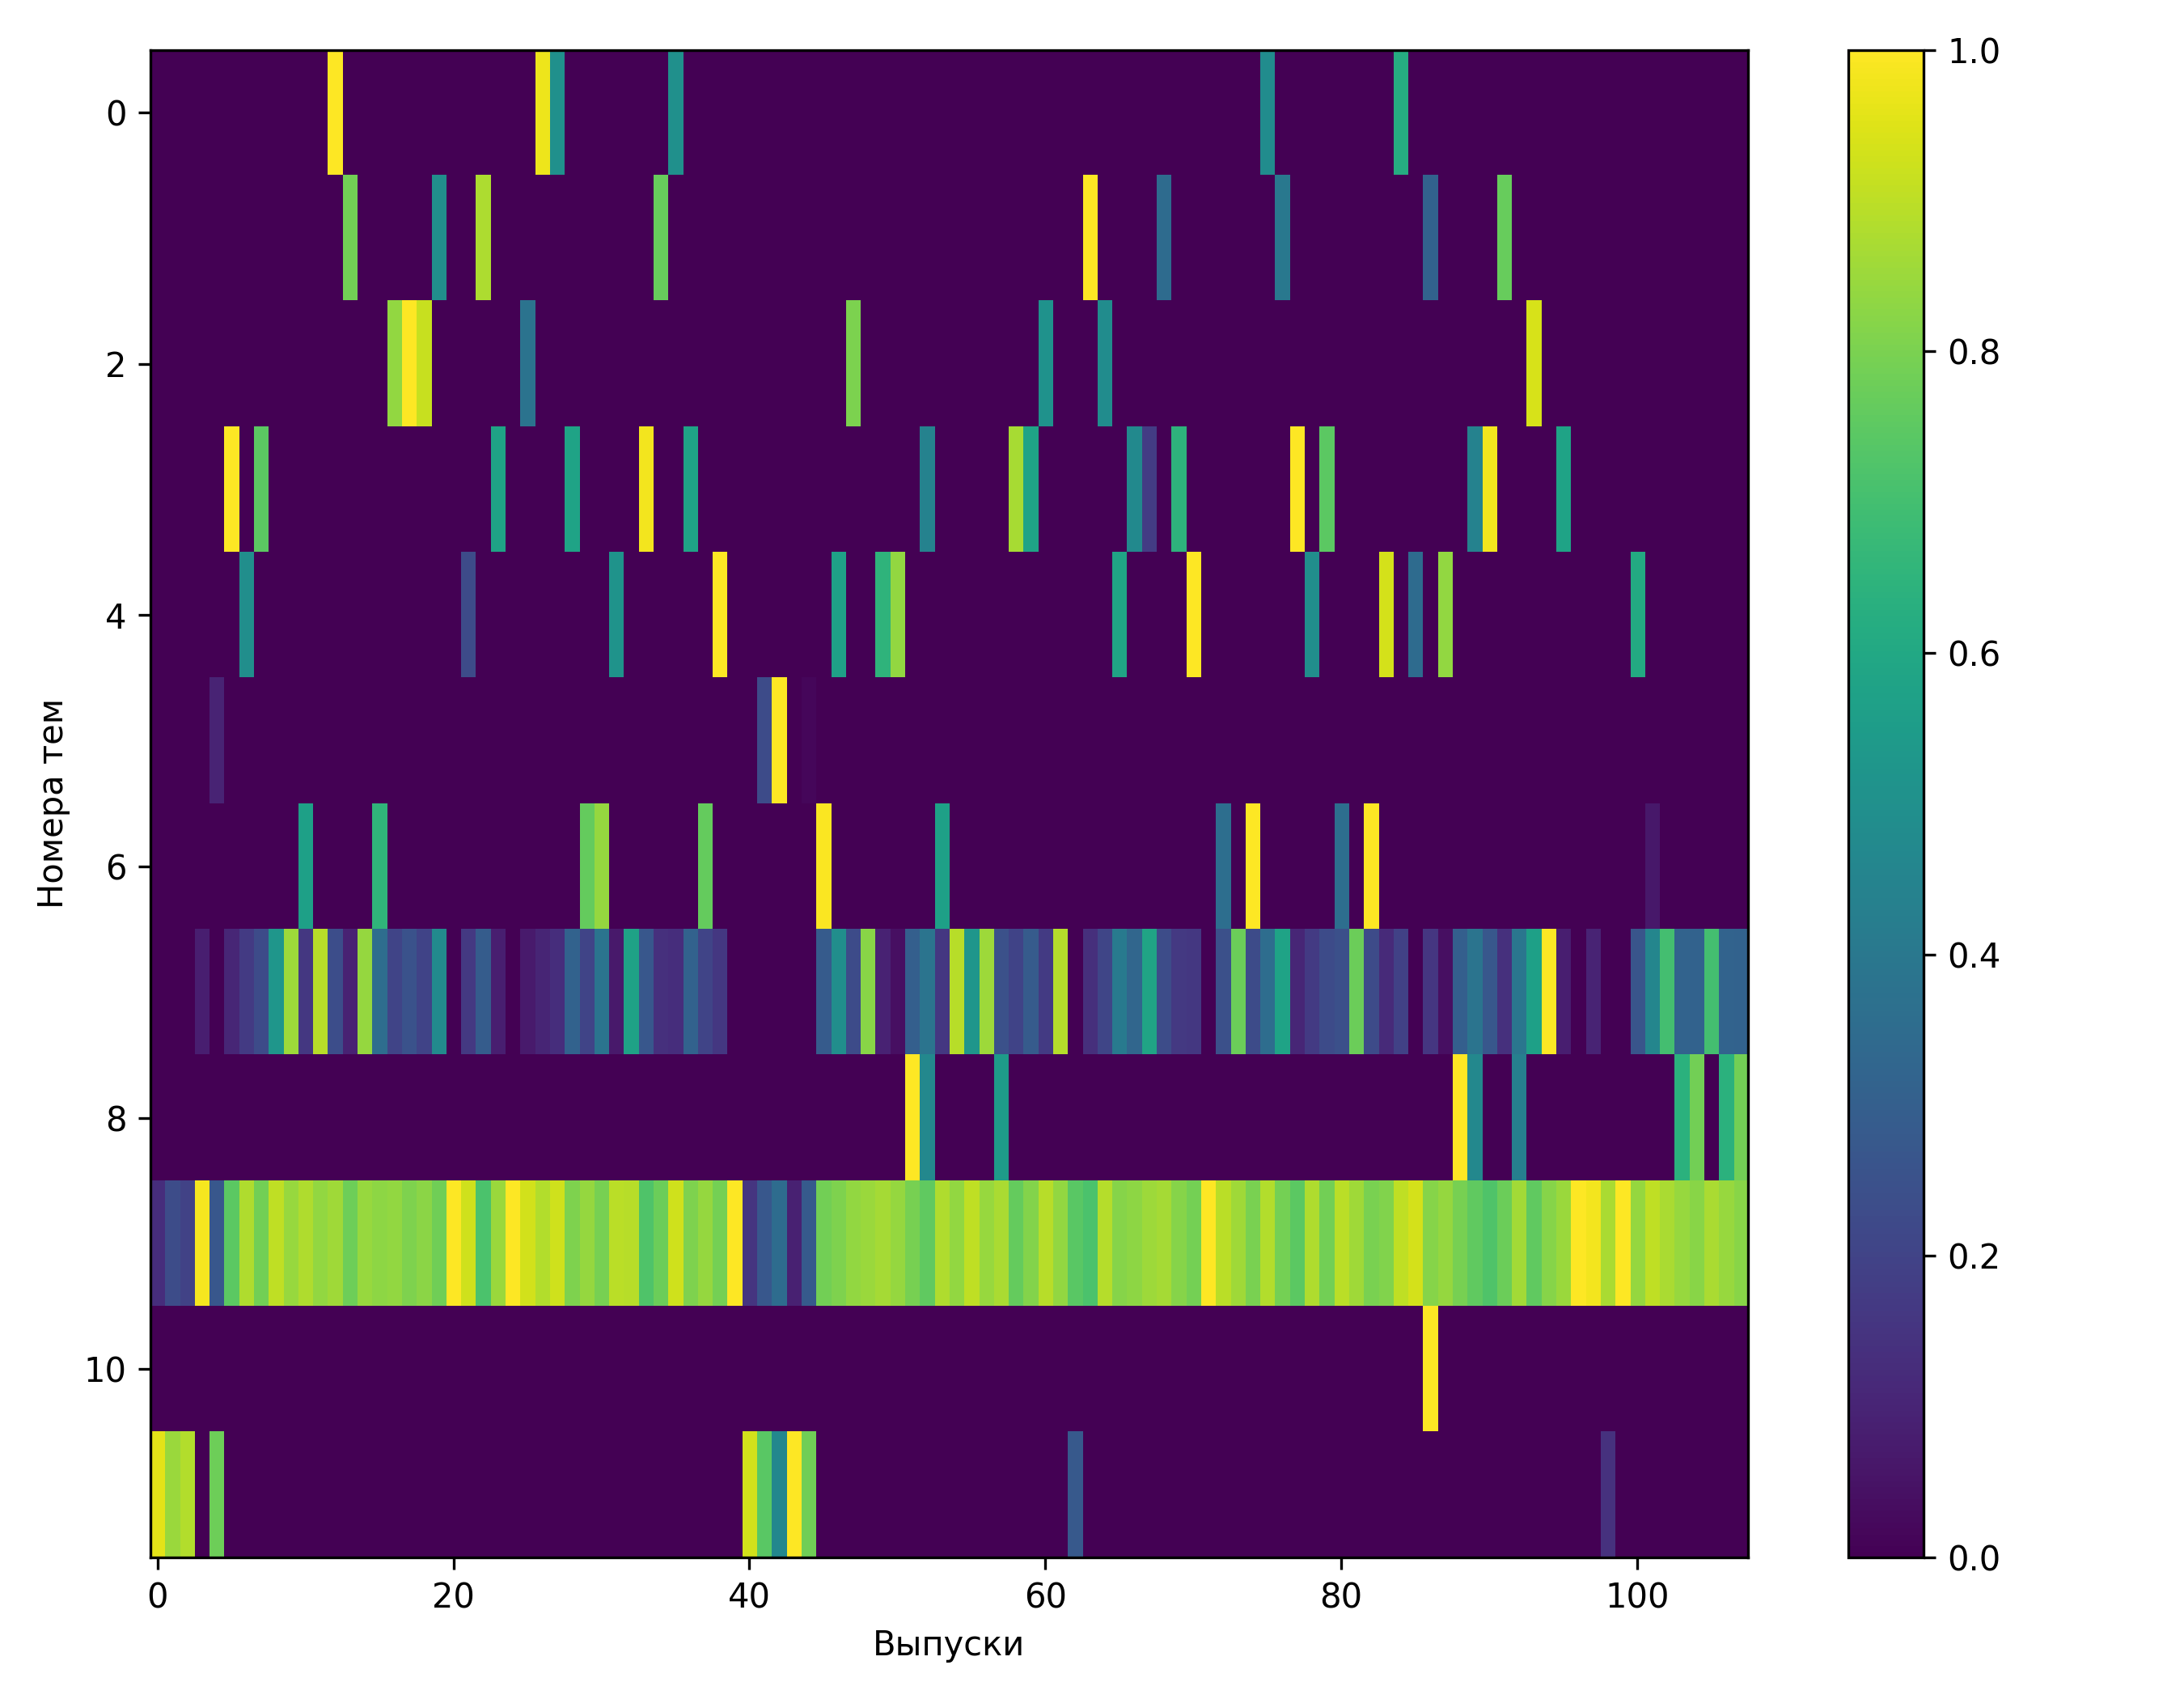
\includegraphics[width=0.8\textwidth]{nx4}
  \label{fig:nx4}
\end{figure} 

На Рис. \ref{fig:nx4} представлена матрица $\Theta$, дающая представление как полученные тематики распределены в каждом из анализируемых выпусков. 
Можно увидеть, что тема с $Тема 9$ представлена во всех выпусках – это общая информация, поздравления, реклама. 
Полученное представление так же позволяет выбирать наиболее релевантные выпуски с определенной темой. 

Важно отметить, что выбранный автором метод показал высокую скорость анализа, что делает его возможным для применения в онлайновых процессах поиска. 
Например, на сайте издательства в качестве средства улучшающего поиск и дающего рекомендации читателям по статьям со схожей тематикой. 
Также следует отметить, что данная методика может быть в дальнейшем усовершенствована и адаптирована для анализа существенно больших массивов динамических данных и выделения ключевых направлений технологического развития как в более широких, так и в более узких областях. 

\section[Скрытые направления исследований]{Разведка скрытых направлений научных исследований в нефтегазовой отрасли}

По оценкам автора более 6 тысяч научно-практических статей публикуется ежегодно на основном нефтегазовом портале https://OnePetro.org. Большинство лиц, принимающих решения в нефтяной индустрии желают быть в курсе основных технологических трендов. Но лишь единицы из них имеют время на то, чтобы прочитать одну-две научных статьи в неделю. Драматически важно чтобы это время было использовано с максимальной эффективностью и выбранные научные статьи представляли действительно сфокусированные исследования высокого качества, а не вторичное перемалывание известных фактов. 

Автор выбрал 1696 статей с сайта OnePetro для углубленного анализа. Эти документы были в формате PDF и нуждались в трансформации в формат пригодный для текстового анализа. Автор использовали библиотеку Apache TIKA для конвертации PDF в текст. В процессе трансформации была восстановлена пунктуация. После получения корпуса текстов необходимо было создать словарь для терминов.

На Рисунке \ref{fig:op3_1} изображена гистограмма частот терминов (слов), которые употреблялись в выбранных статьях и доля выбранных терминов для дальнейшего анализа. С помощью такой выборки автор избавилися от слов с низкими и высокими частотами употребления в коллекции текстов.

\begin{figure}[H]
  \caption{Распределение частот терминов в корпусе текстов.}
  \centering
    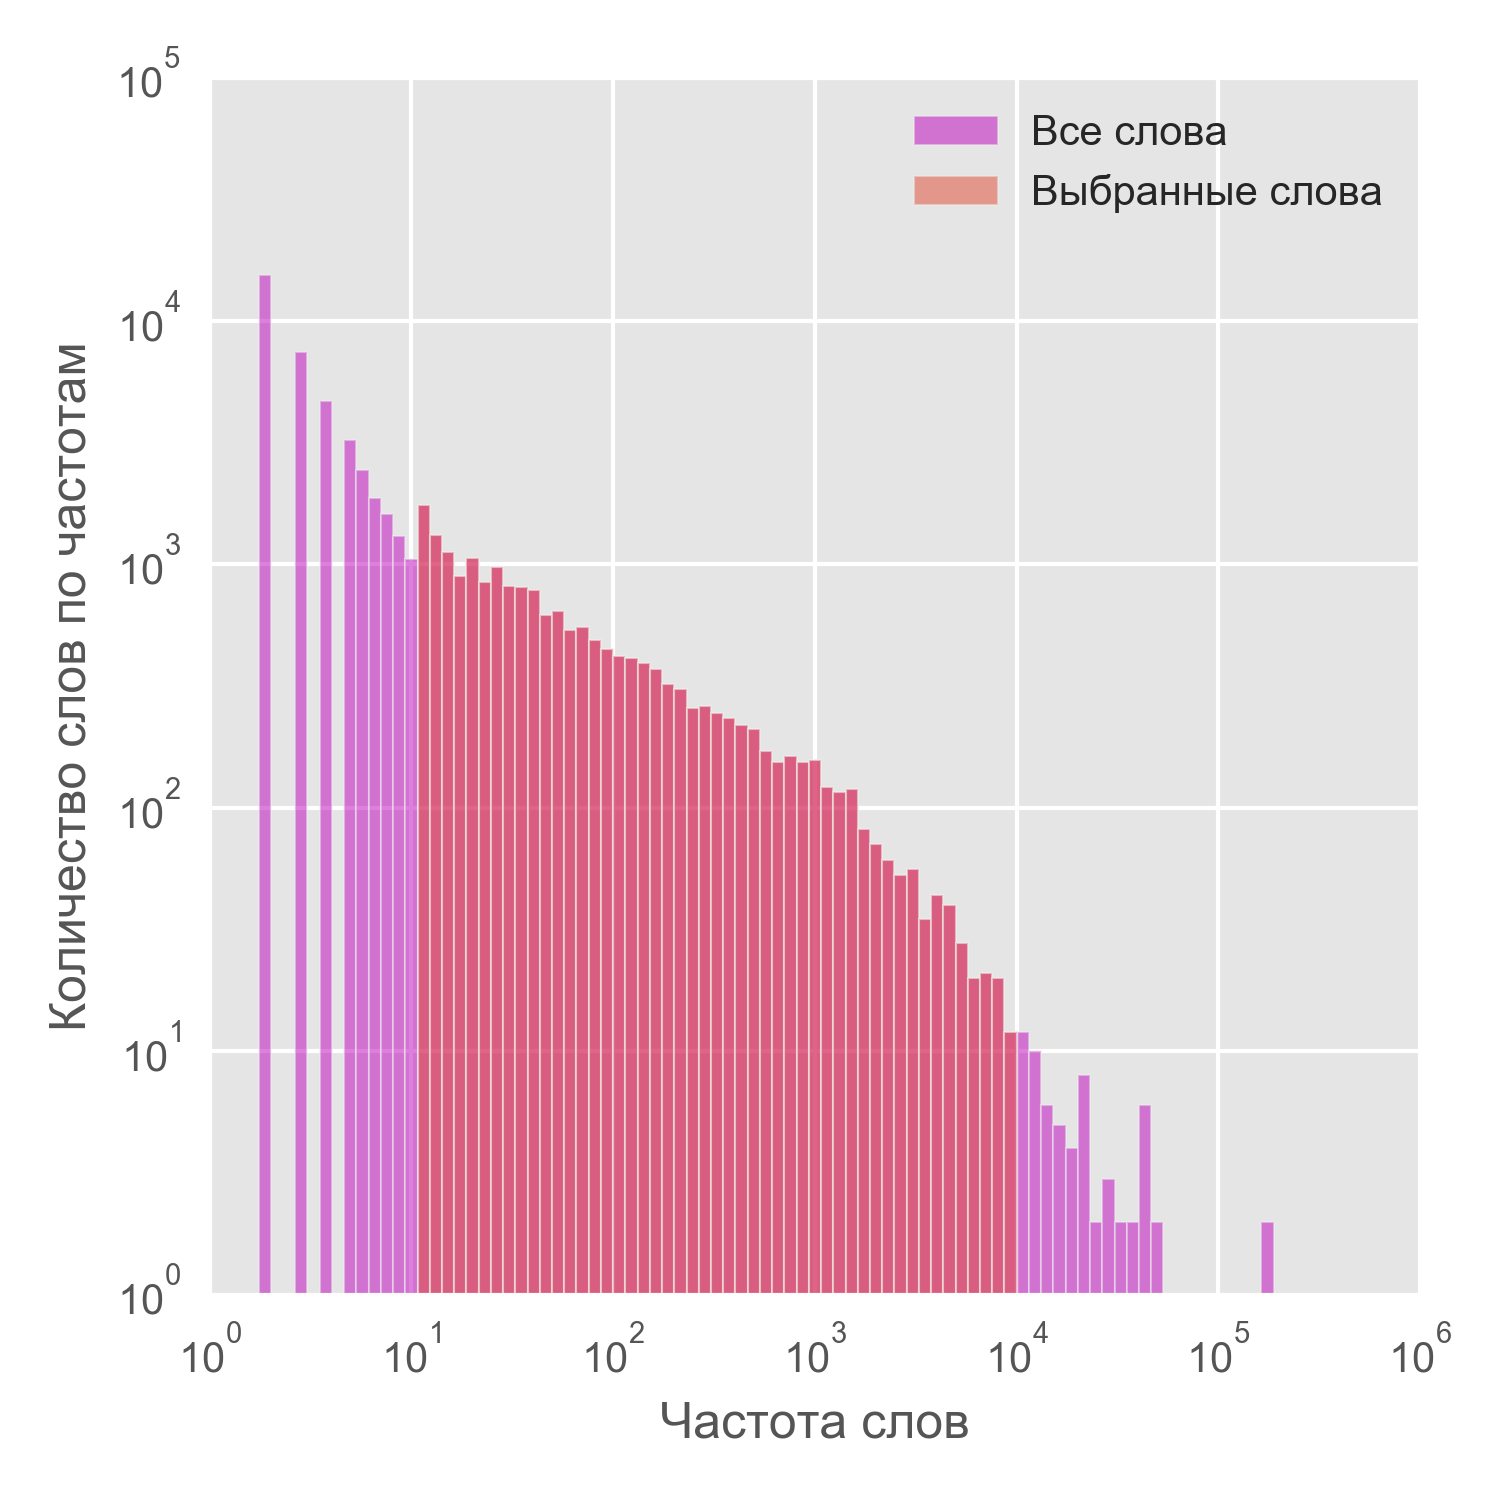
\includegraphics[width=0.8\textwidth]{op3_fig1rus}
  \label{fig:op3_1}
\end{figure}  

В соответствии с методикой, изложенной в разделе \ref{sec:topicmodel}, в начале автор произвел тренировку PLSA topic model чтобы определить
скорость сходимости по метрике \emph{Perplexity}. Зависимость \emph{Perplexity} от количества проходов отображена на Рисунке \ref{fig:op3_2}.

\begin{figure}[H]
  \caption{Зависимость Perplexity от количества проходов.}
  \centering
    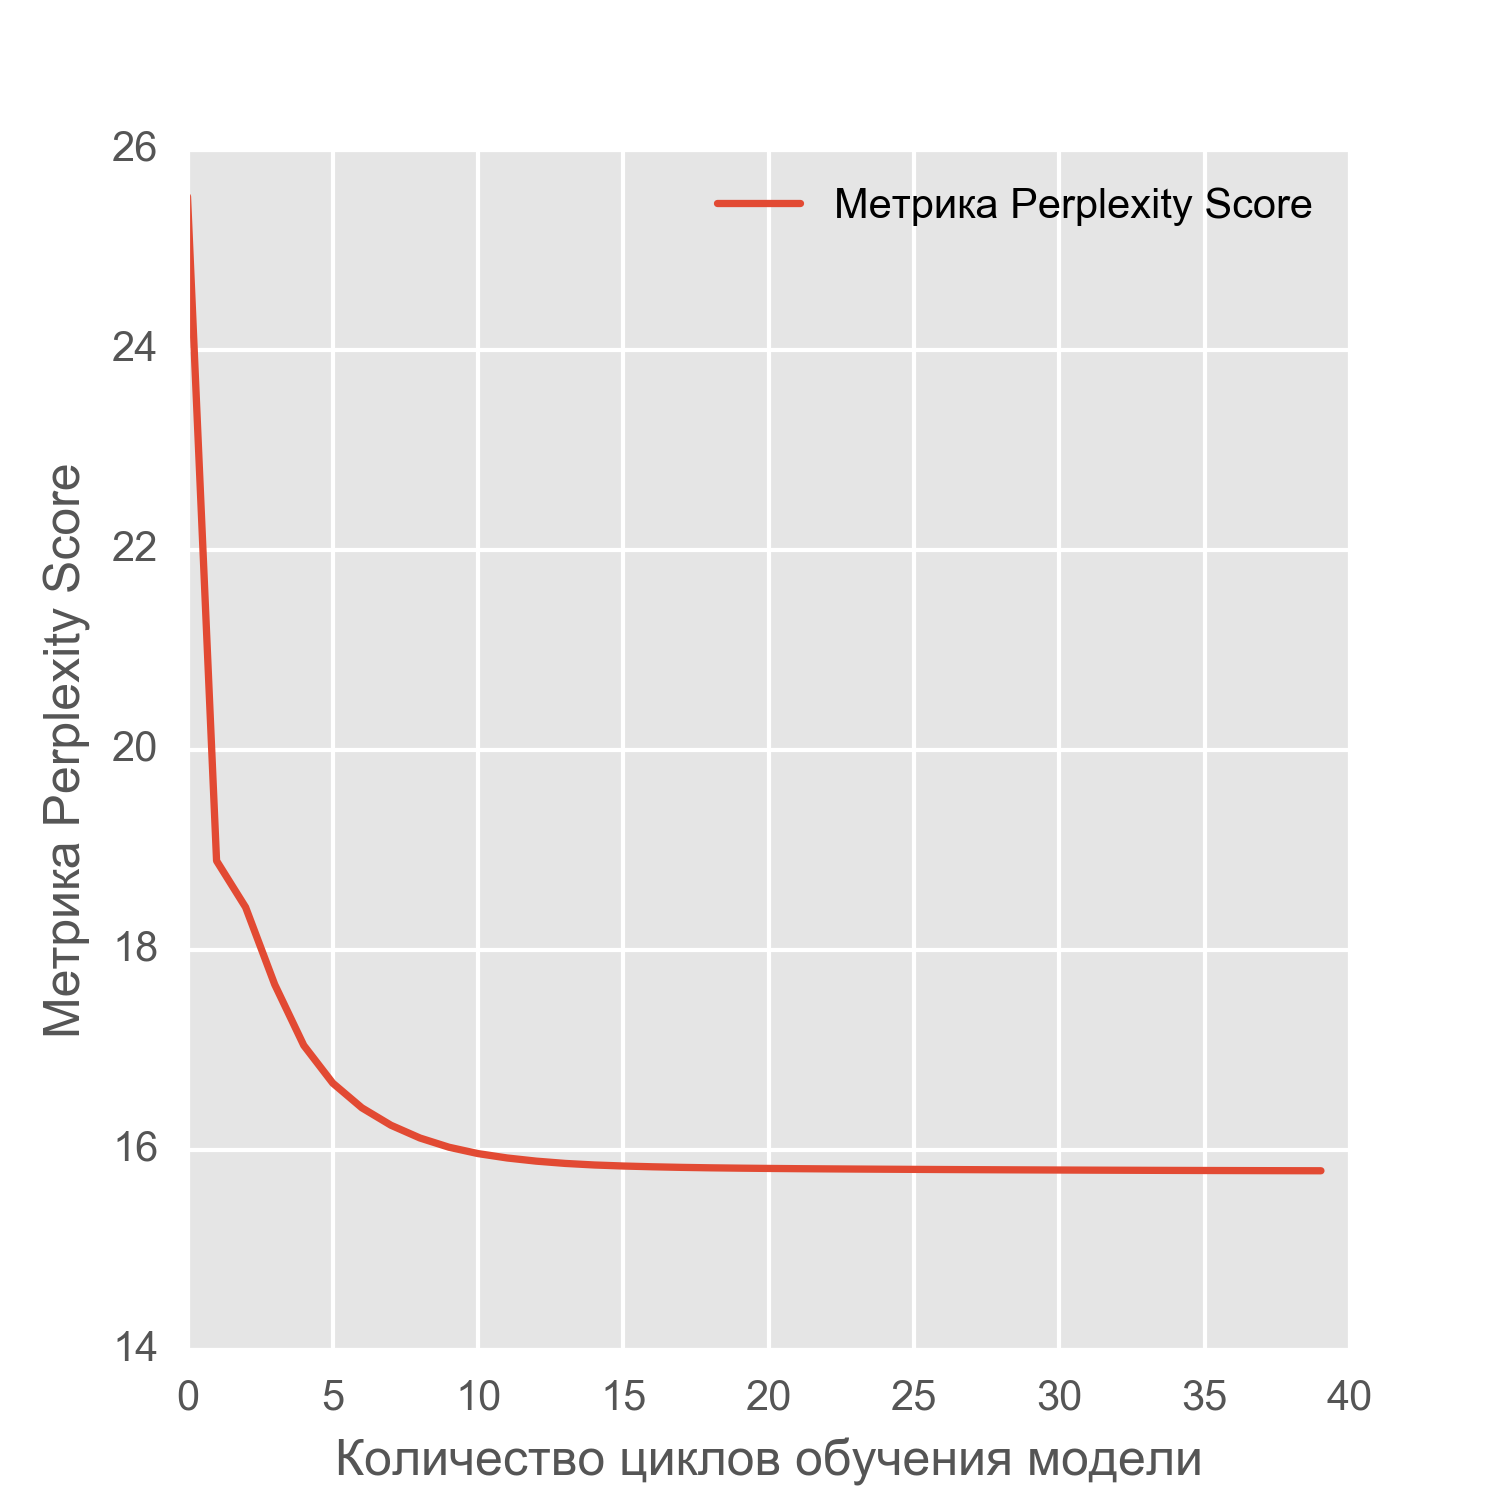
\includegraphics[width=0.8\textwidth]{op3_fig2rus}
  \label{fig:op3_2}
\end{figure}  

Из рисунка \ref{fig:op3_2} видно, что модель хорошо сходится уже на 20 прогонах.

Для дальнейшего обучения к модели были добавлены следующие регуляризаторы:

\begin{enumerate}
\def\labelenumi{\arabic{enumi}.}
\tightlist
\item Sparse Theta -- для увеличения разрежённости матрицы $\Theta$ для основных тематик,
\item Sparse Phi -- для увеличения разрежённости матрицы $\Phi$ для основных тематик,
\item Smooth Theta -- для уплотнения матрицы $\Theta$ для шумовых тематик,
\item Smooth Phi -- для уплотнения матрицы $\Phi$ для шумовых тематик.
\end{enumerate}

Для определения параметров регуляризаторов были проведены следующие пробные эксперименты по обучению модели. 
Результаты этих пробных экспериментов оценивались по метрикам разрежённости матриц $\Phi$ и $\Theta$ . 
Для уплотнения матриц и предполагается использовать полученные параметры $\tau$ с  обратным знаком.

На рисунке \ref{fig:op3_3} приведена зависимость разрежённости матрицы для нескольких значений параметра регуляризации $ \tau $.
\begin{figure}[H]
  \caption{Зависимость разрежённости матрицы $ \Phi $ для нескольких значений параметра регуляризации $ \tau $.}
  \centering
    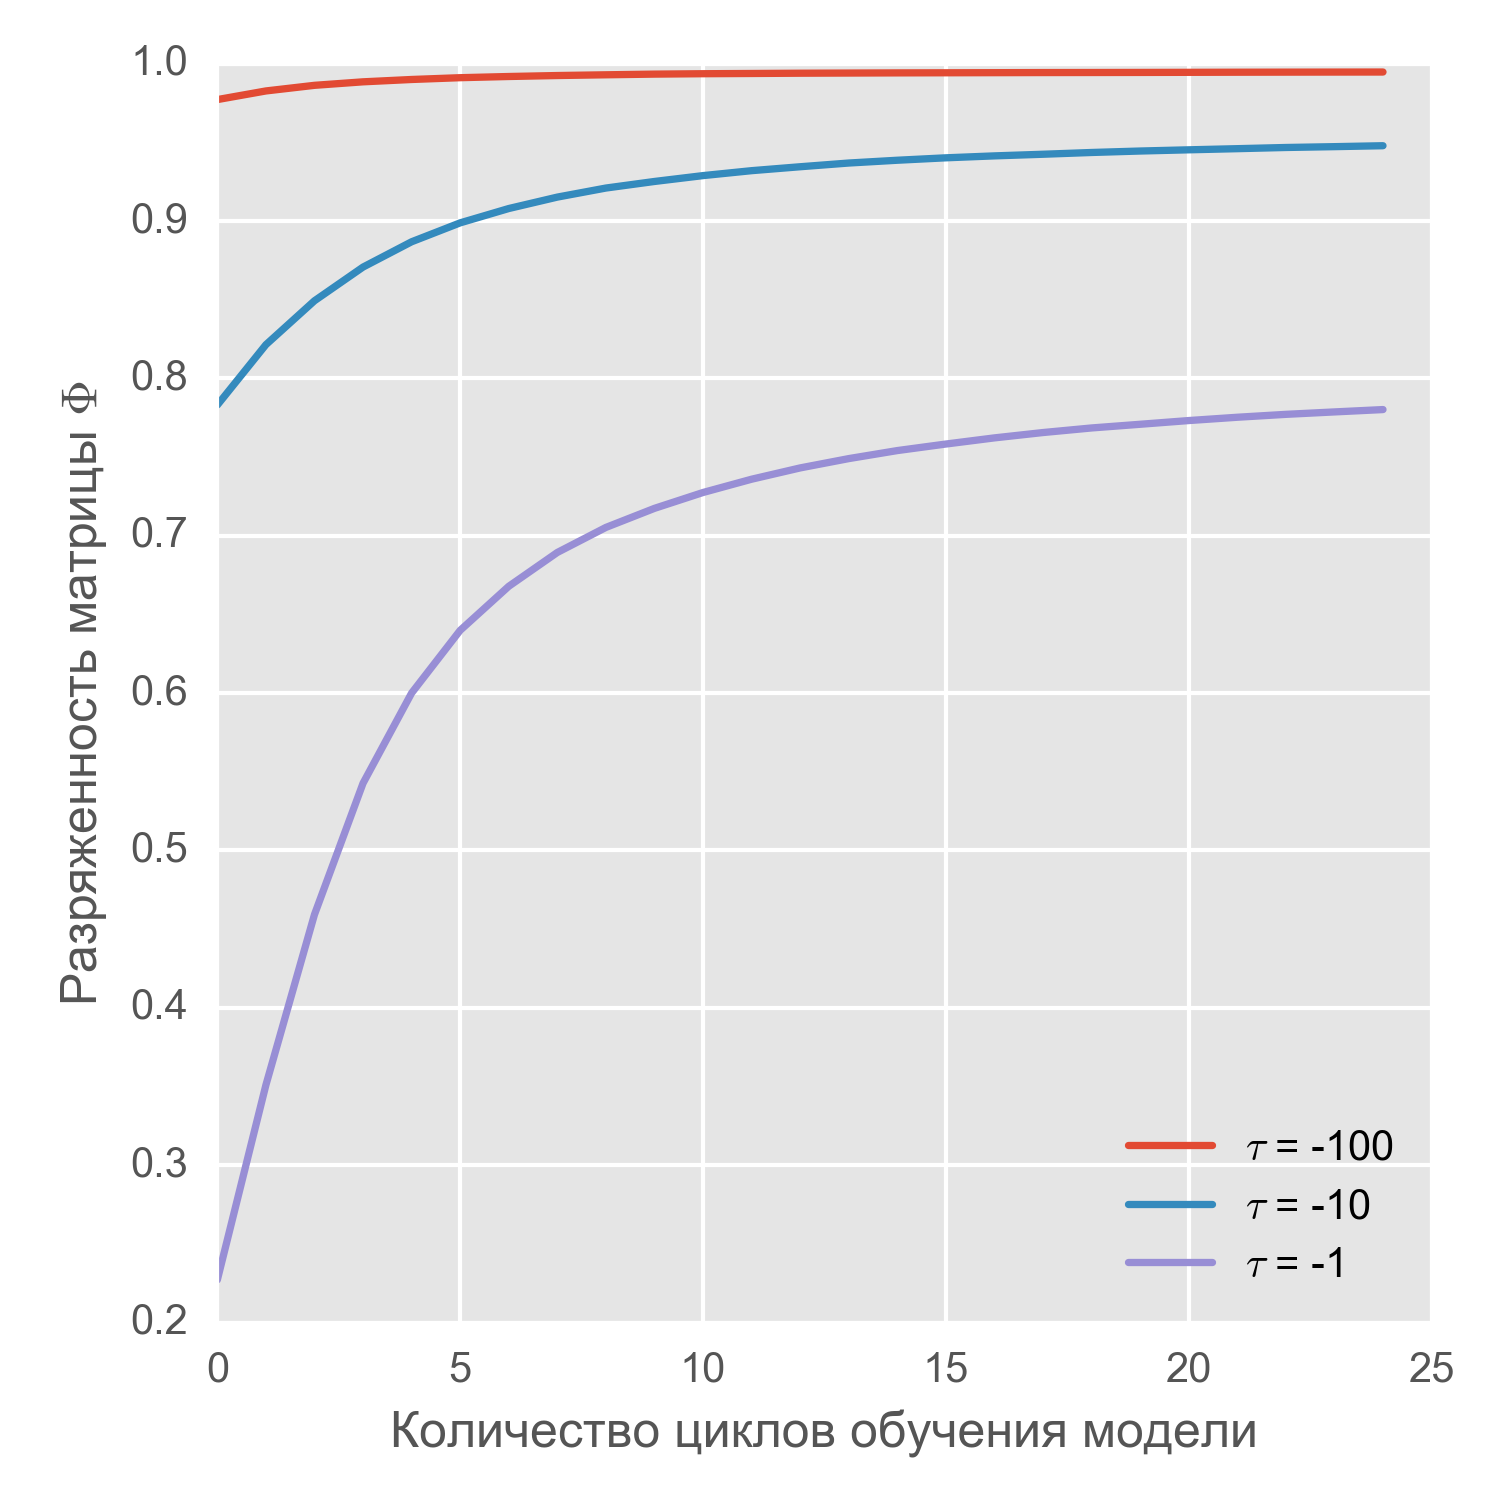
\includegraphics[width=0.8\textwidth]{op3_fig3rus}
  \label{fig:op3_3}
\end{figure}  

На основании зависимости отображенной на рисунке \ref{fig:op3_3} для дальнейших экспериментов было
выбрано значение $ \tau = -10 $. При таком значении $ \tau $ после 25 прогонов в матрице $\Phi $ остается 92\% нулевых значений.

На рисунке \ref{fig:op3_4}  приведена зависимость разрежённости матрицы $\Theta$  для нескольких значений параметра регуляризации $ \tau $.

\begin{figure}[H]
  \caption{Зависимость разрежённости матрицы $ \Theta $ для нескольких значений параметра регуляризации $ \tau $.}
  \centering
    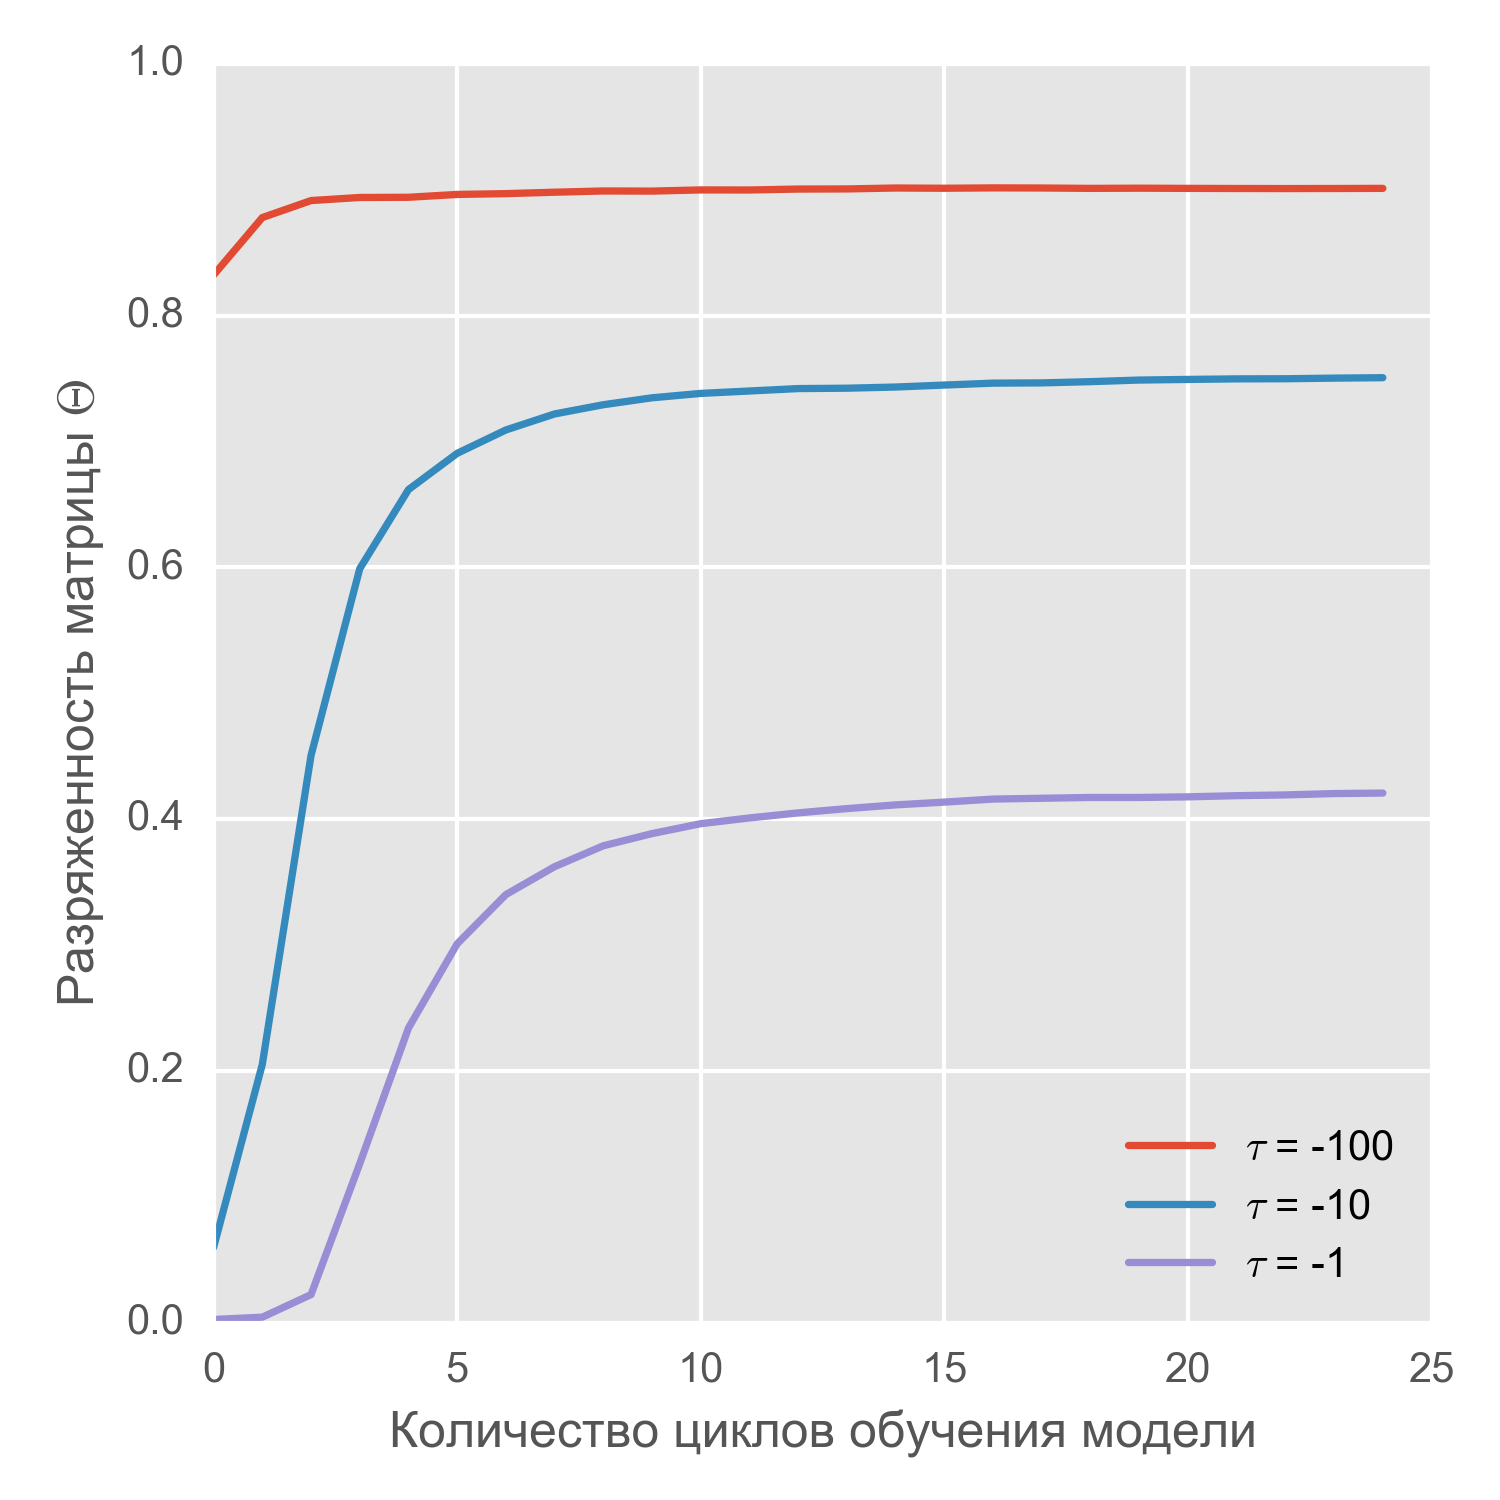
\includegraphics[width=0.8\textwidth]{op3_fig4rus}
  \label{fig:op3_4}
\end{figure}  

На основании зависимости отображенной на рисунке  \ref{fig:op3_4}  для дальнейших экспериментов было выбрано значение $ \tau  = 10 $. 
При таком значении $ \tau $ после 25 прогонов в матрице остается 78\% нулевых значений.

Для того, чтобы качественно оценить полученную тематическую модель автор применил метод визуальных оценок качества кластеризации.
Рассмотрим темы в тематической модели как кластеры. Тогда хорошо выделенная тема должна описываться ``близкими'' словами и отстоять
``далеко'' от слов, образующих другие темы.

Чтобы сравнивать ``близость'' и ``удаленность'' слова были представлены в виде векторов с помощью алгоритмов FastText и GloVe. Для отображения
полученных векторов были использованы два алгоритма уменьшения размерности: TSNE и MDS.

Алгоритм TSNE имеет несколько значимых параметров, таких как метрика,
perplexity и learning rate. Автор рассмотрел значения perplexity от 5
до 50 с шагом 5 и перебрал следующие метрики расстояний: cosine и euclidean. 
Наиболее наглядные результаты представлены на \ref{fig:op3_5} и \ref{fig:op3_6}. 

\begin{figure}[H]
  \caption{Кластеры слов по тематикам. Векторы слов получены с помощью FastText. Визуализация получена с помощью TSNE с параметрами preplexity=30 и метрикой cosine.}
  \centering
    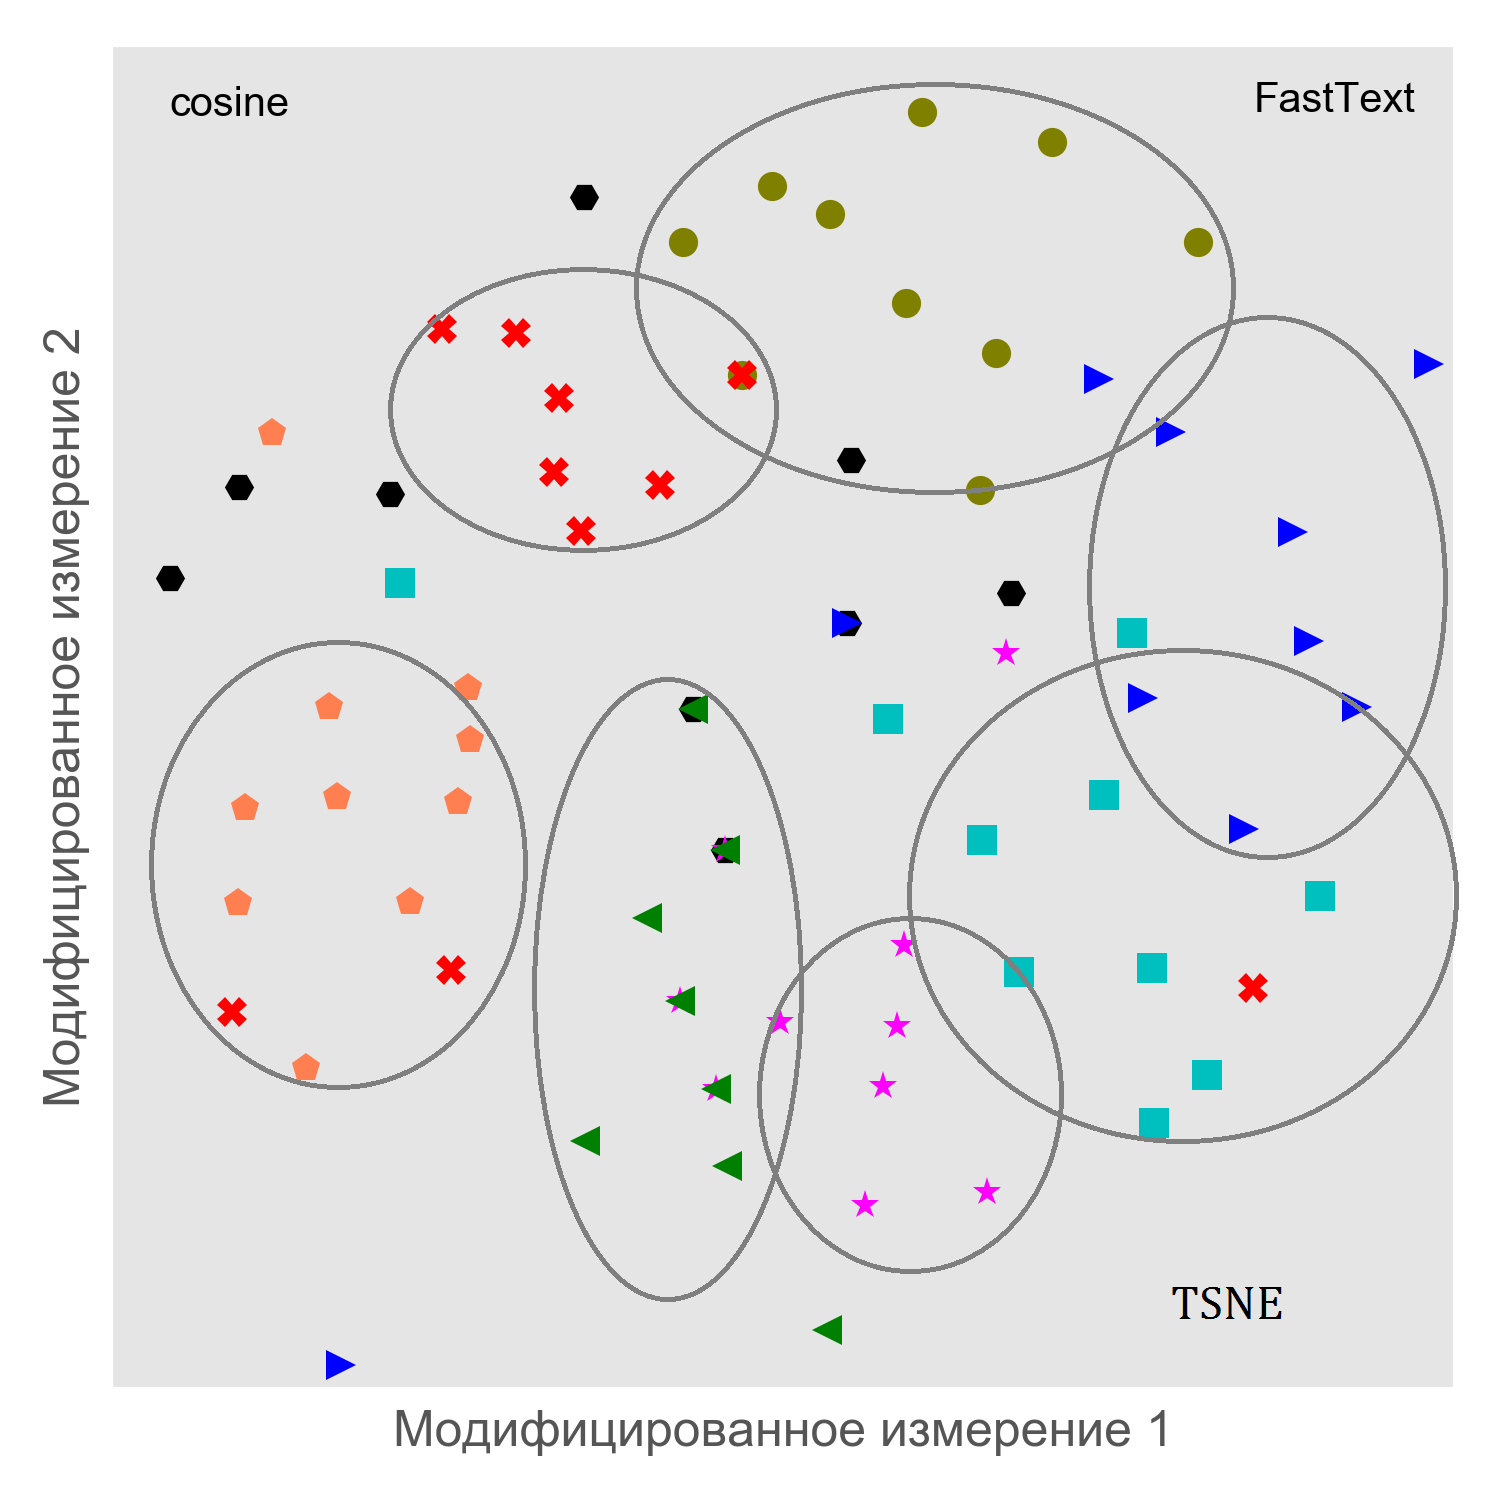
\includegraphics[width=0.8\textwidth]{op3_fig5rus}
  \label{fig:op3_5}
\end{figure}

\begin{figure}[H]
  \caption{Кластеры слов по тематикам. Векторы слов получены с помощью GloVe. Визуализация получена с помощью TSNE с параметрами preplexity=30 и метрикой cosine.}
  \centering
    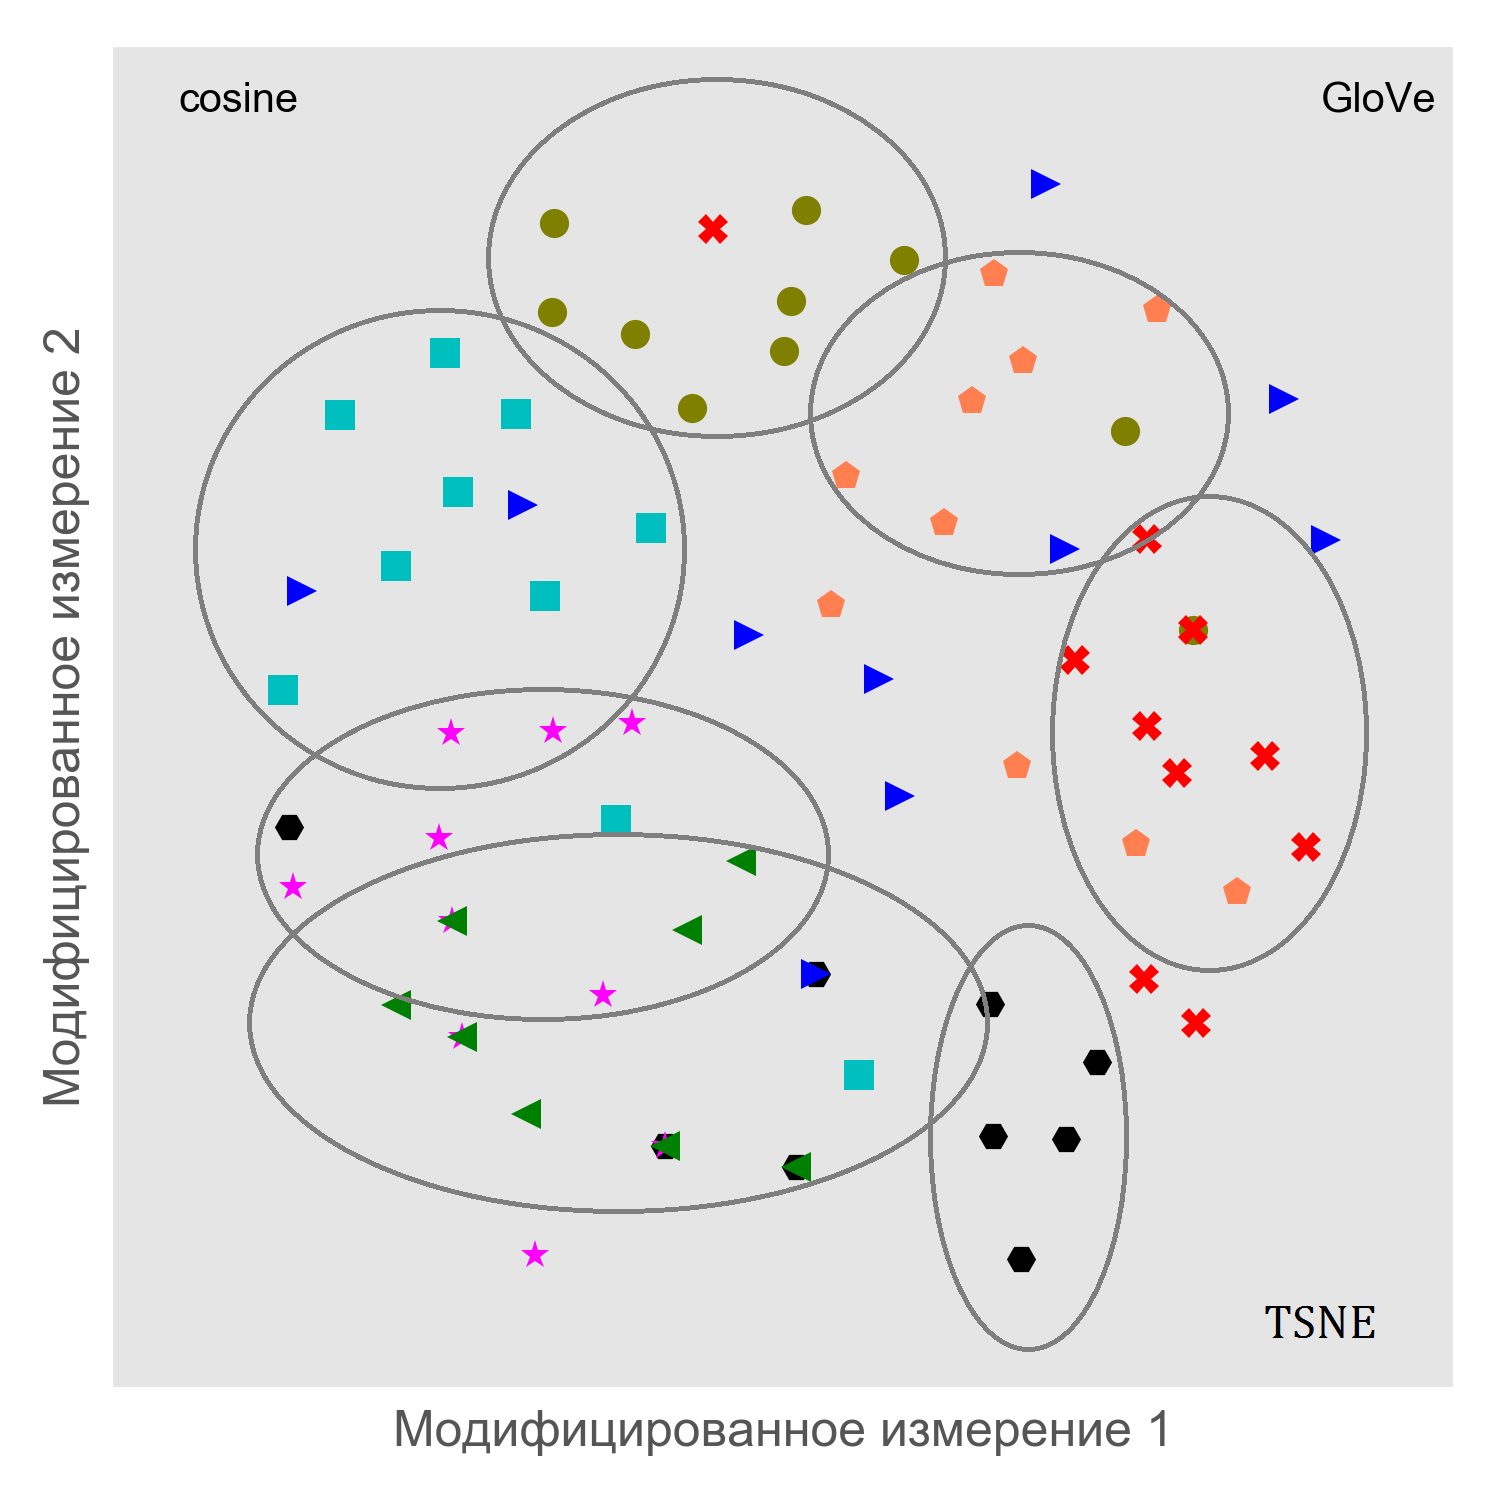
\includegraphics[width=0.8\textwidth]{op3_fig6rus}
  \label{fig:op3_6}
\end{figure}

На основе \ref{fig:op3_5} и \ref{fig:op3_6} можно наблюдать группировки слов, образующих тематики. Отметим, что расстояния при трансформации
векторного пространства методом TSNE не сохраняются, но сохраняются пропорции расстояний.

Преобразование векторного пространства с помощью метода MDS отображены  на \ref{fig:op3_7} и \ref{fig:op3_8}.

\begin{figure}[H]
  \caption{Кластеры слов по тематикам. Векторы слов получены с помощью FastText. Визуализация получена с помощью MDS.}
  \centering
    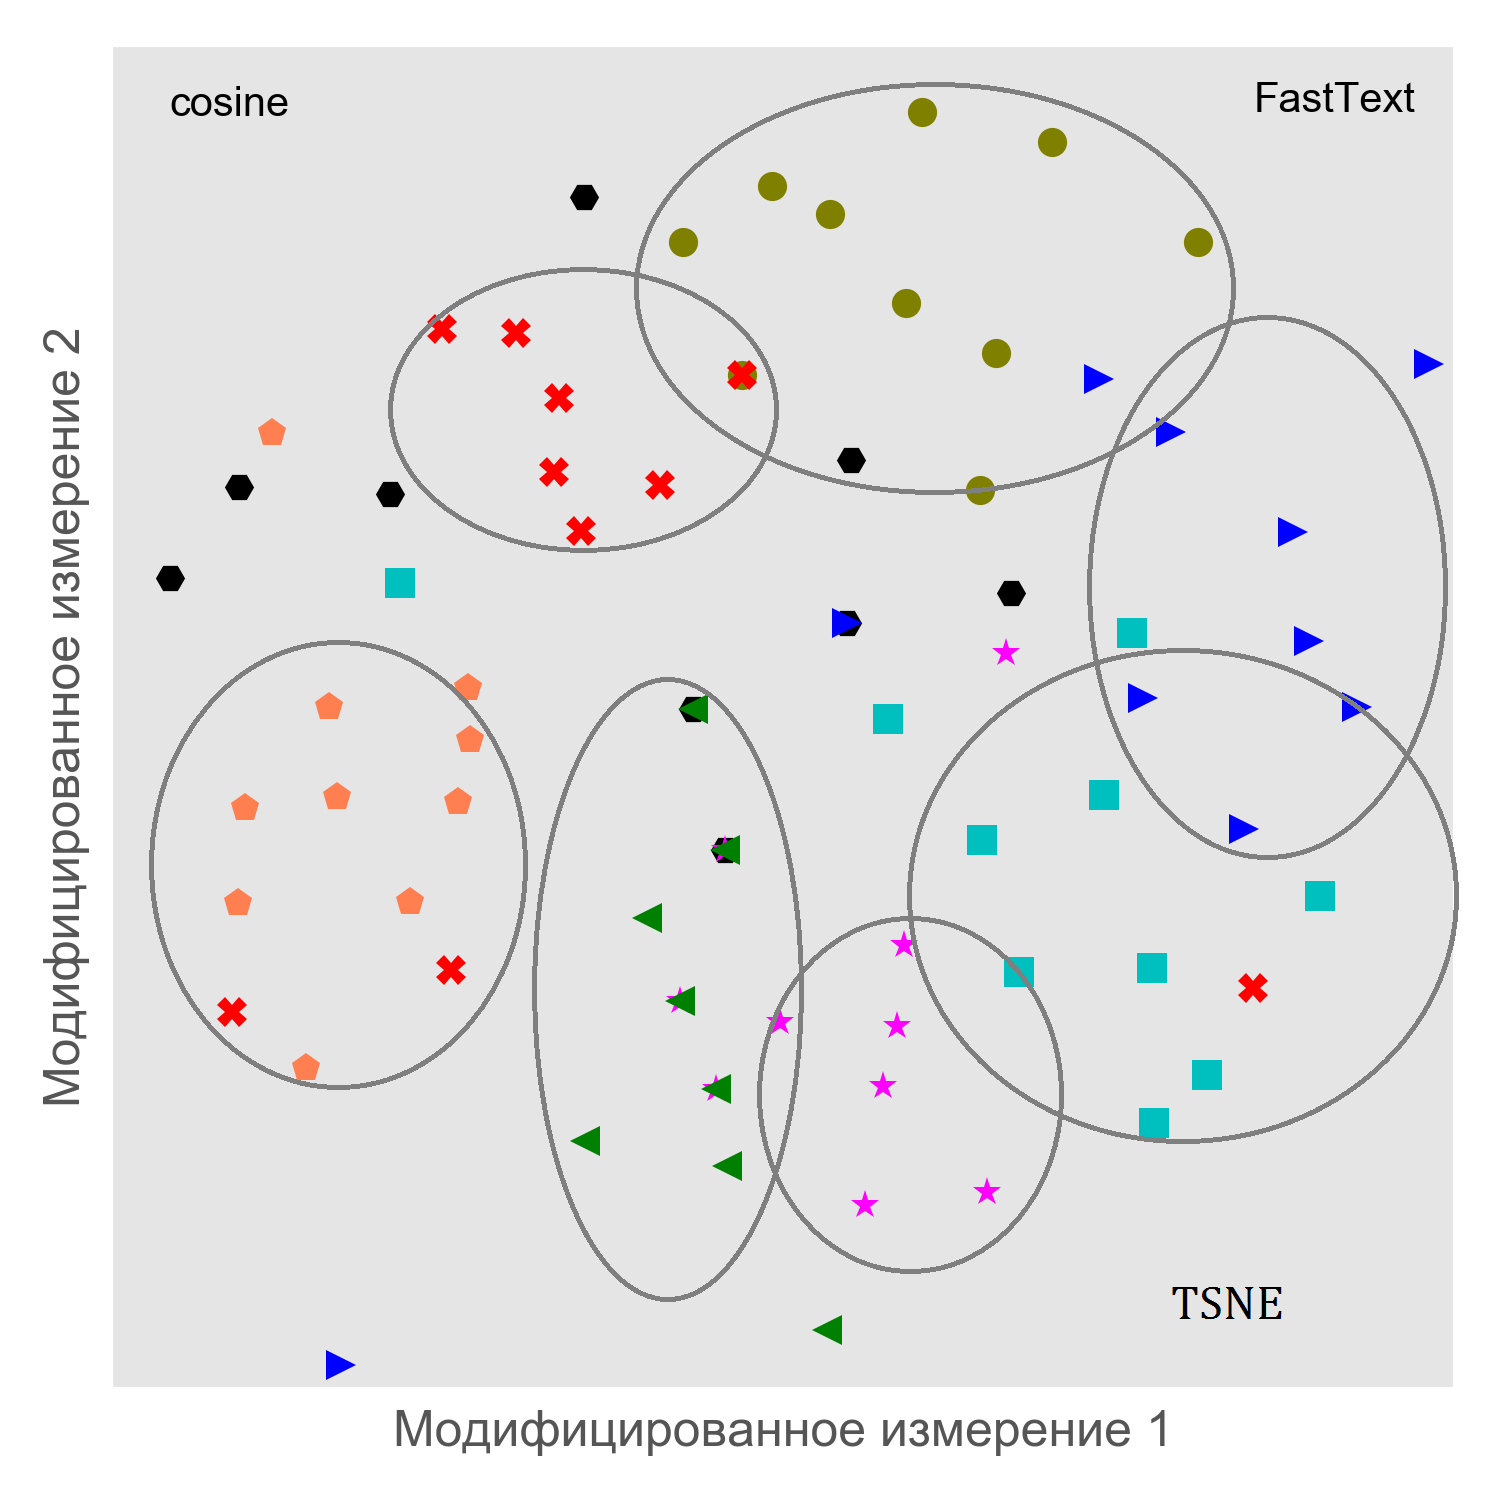
\includegraphics[width=0.8\textwidth]{op3_fig5rus}
  \label{fig:op3_7}
\end{figure}

\begin{figure}[H]
  \caption{Кластеры слов по тематикам. Векторы слов получены с помощью GloVe. Визуализация получена с помощью MDS.}
  \centering
    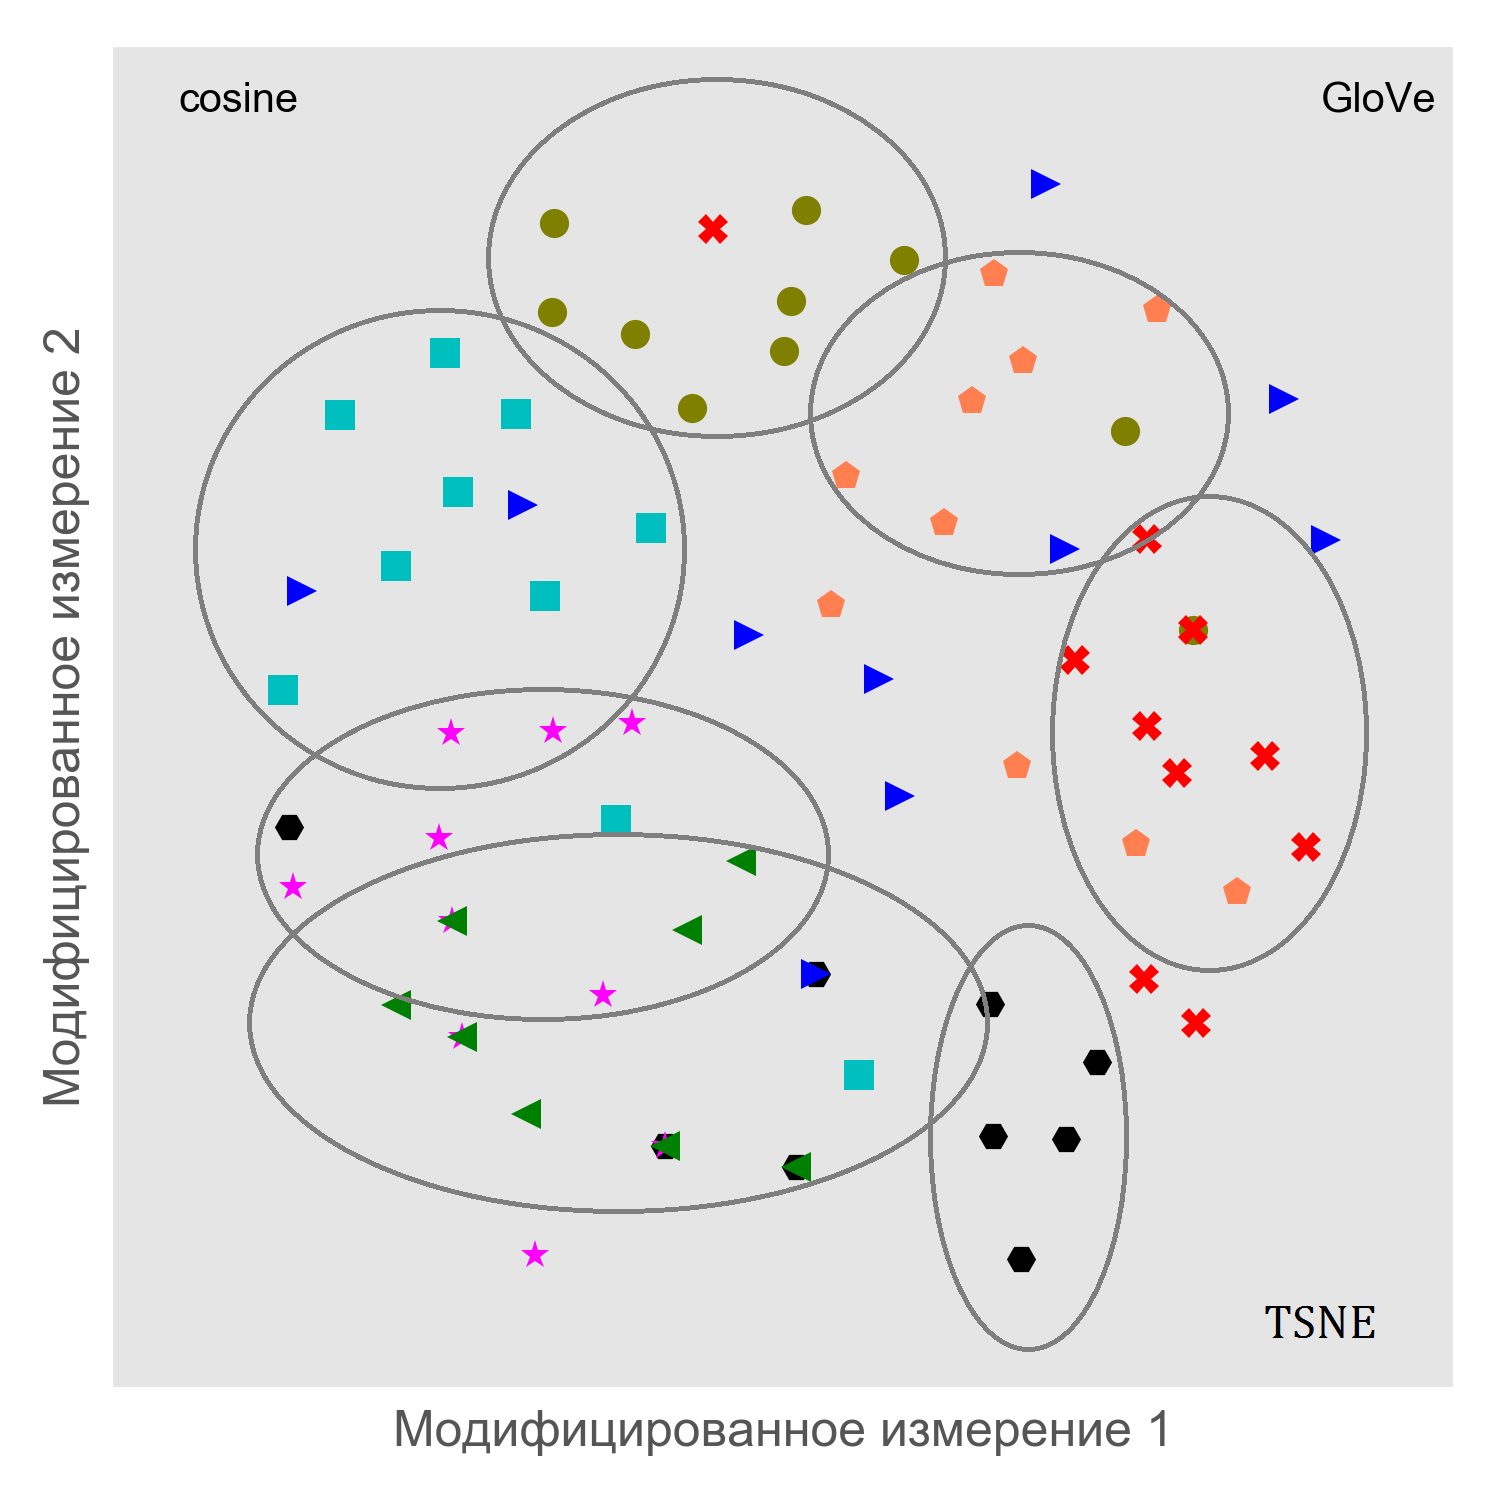
\includegraphics[width=0.8\textwidth]{op3_fig6rus}
  \label{fig:op3_8}
\end{figure}

На рисунках \ref{fig:op3_7} и \ref{fig:op3_8} можно видеть группировку слов, образующих тематики. 
Алгоритм MDS использует евклидову метрику для вычисления расстояний.

Полученные с помощью MDS и TSNE результаты для FastText и GloVe
показывают наличие кластеров слов , соответствующих тематикам. Так же мы
видим наличие шумовых слов в тематиках.

В таблице \ref{tab:op3_1}  представлены top10 терминов, образующих основные тематики до регуляризации.

\begin{table}[H]
\centering
\caption{Top10 терминов, образующих тематики до регуляризации.}
\label{tab:op3_1}
\resizebox{\textwidth}{!}{%
\begin{tabular}{lllllllll}
Топик & sbj0 & sbj1 & sbj2 & sbj3 & sbj4 & sbj5 & sbj6 & sbj7 \\
Терм1 & liquid & sand & stress & injection & corrosion & casing & injection & safety \\
Терм2 & equation & shale & fractures & history & nace & mud & recovery & management \\
Терм3 & velocity & porosity & hydraulic & matrix & samples & cement & steam & risk \\
Терм4 & pipe & logging & fracturing & optimization & concentration & hole & viscosity & assessment \\
Терм5 & experimental & pore & proppant & recovery & acid & tubing & core & human \\
Терм6 & eq & samples & shale & porosity & treatment & string & heavy & health \\
Терм7 & coefficient & core & stage & linear & steel & drill & injected & company \\
Терм8 & multiphase & log & treatment & matching & ph & bit & polymer & team \\
Терм9 & equations & sample & conductivity & match & inhibitor & completion & flooding & equipment \\
Терм10 & mass & logs & stimulation & cumulative & chemical & mpd & solvent & environmental
\end{tabular}%
}
\end{table}

В таблице \ref{tab:op3_2} представлены top10 терминов, образующих основные тематики после применения обучения с регуляризацией.

\begin{table}[H]
\centering
\caption{Top10 терминов, образующихосновные тематики после применения обучения с регуляризацией.}
\label{tab:op3_2}
\resizebox{\textwidth}{!}{%
\begin{tabular}{lllllllll}
Топик & sbj0 & sbj1 & sbj2 & sbj3 & sbj4 & sbj5 & sbj6 & sbj7 \\
Терм1 & liquid & shale & fracturing & injection & corrosion & casing & recovery & safety \\
Терм2 & pipeline & porosity & proppant & fractures & nace & cement & injection & management \\
Терм3 & pipe & logging & hydraulic & shale & concentration & mud & steam & risk \\
Терм4 & velocity & sand & stress & matrix & samples & hole & core & human \\
Терм5 & multiphase & pore & fractures & hydraulic & inhibitor & mpd & viscosity & health \\
Терм6 & slug & samples & stage & recovery & acid & bit & flooding & business \\
Терм7 & friction & core & shale & fractured & ph & drill & solvent & assessment \\
Терм8 & bhr & spwla & treatment & bakken & steel & string & heavy & training \\
Терм9 & group & clay & conductivity & porosity & houston & pipe & saturation & company \\
Терм10 & holdup & symposium & stages & unconventional & iron & liner & surfactant & activities
\end{tabular}%
}
\end{table}

Из таблиц \ref{tab:op3_1} и \ref{tab:op3_2} мы видим, что основные термины,
формирующие тематики устойчивы к процессам регуляризации. Качество
интерпретируемости тематик улучшается с регуляризацией за счет появления
более конкретных терминов.

Так же представляет интерес поведение тематик для отбора шумовых
терминов. В таблице приведены шумовые тематики до и после регуляризации.

\begin{table}[H]
\centering
\caption{Top10 терминов, образующих шумовые тематики до и послеприменения обучения с регуляризацией.}
\label{tab:op3_3}
\resizebox{\textwidth}{!}{%
\begin{tabular}{|l|l|l|l|}
\hline
\multicolumn{2}{|l|}{\textbf{До регуляризации}} & \multicolumn{2}{l|}{\textbf{После регуляризации}} \\ \hline
\textbf{nz0} & \textbf{nz1} & \textbf{nz0} & \textbf{nz1} \\ \hline
pump & wave & pump & stress \\ \hline
pipeline & seismic & sand & equation \\ \hline
esp & seg & completion & seismic \\ \hline
power & frequency & injection & wave \\ \hline
subsea & velocity & tubing & velocity \\ \hline
operating & waves & equipment & numerical \\ \hline
lift & amplitude & operating & x \\ \hline
equipment & x & downhole & pore \\ \hline
installation & elastic & power & our \\ \hline
liquid & offshore & esp & direction \\ \hline
\end{tabular}%
}
\end{table}

Примечательно, что в шумовые тематики попала тема Сейсмики (nz1).
Согласно мнению эксперта сейсмике относятся слова seismic, wave,
velocity, elastic, seg, frequency и amplitude. Статьи по сейсмике мало
представлены в библиотеке OnePetro и действительно могут быть отнесены к
второстепенным. После обучения с регуляризацией в nz1 добавились
несколько терминов связанных с вычислениями, но тема сейсмики осталась.
В частности, термин offshore ушел в основные тематики. С тематикой nz0
все достаточно однозначно. В нее попали часто употребляемые слова,
которые не являются на самом деле шумом.

Рассмотрим результат отнесения моделью документов к определенным
тематикам. Распределение тематик для каждого документа отражены в матрице
$\Theta$ . Для получения более общего представления о происходящем преобразовании
матрицы авторы представили ее вид до (Рис. \ref{fig:op3_9}) и после (Рис. \ref{fig:op3_10}) регуляризации в
виде 2D-карт.

\begin{figure}[H]
  \caption{Матрица  $ \Theta $ до регуляризации. По оси x отложены номера документов из коллекции.}
  \centering
    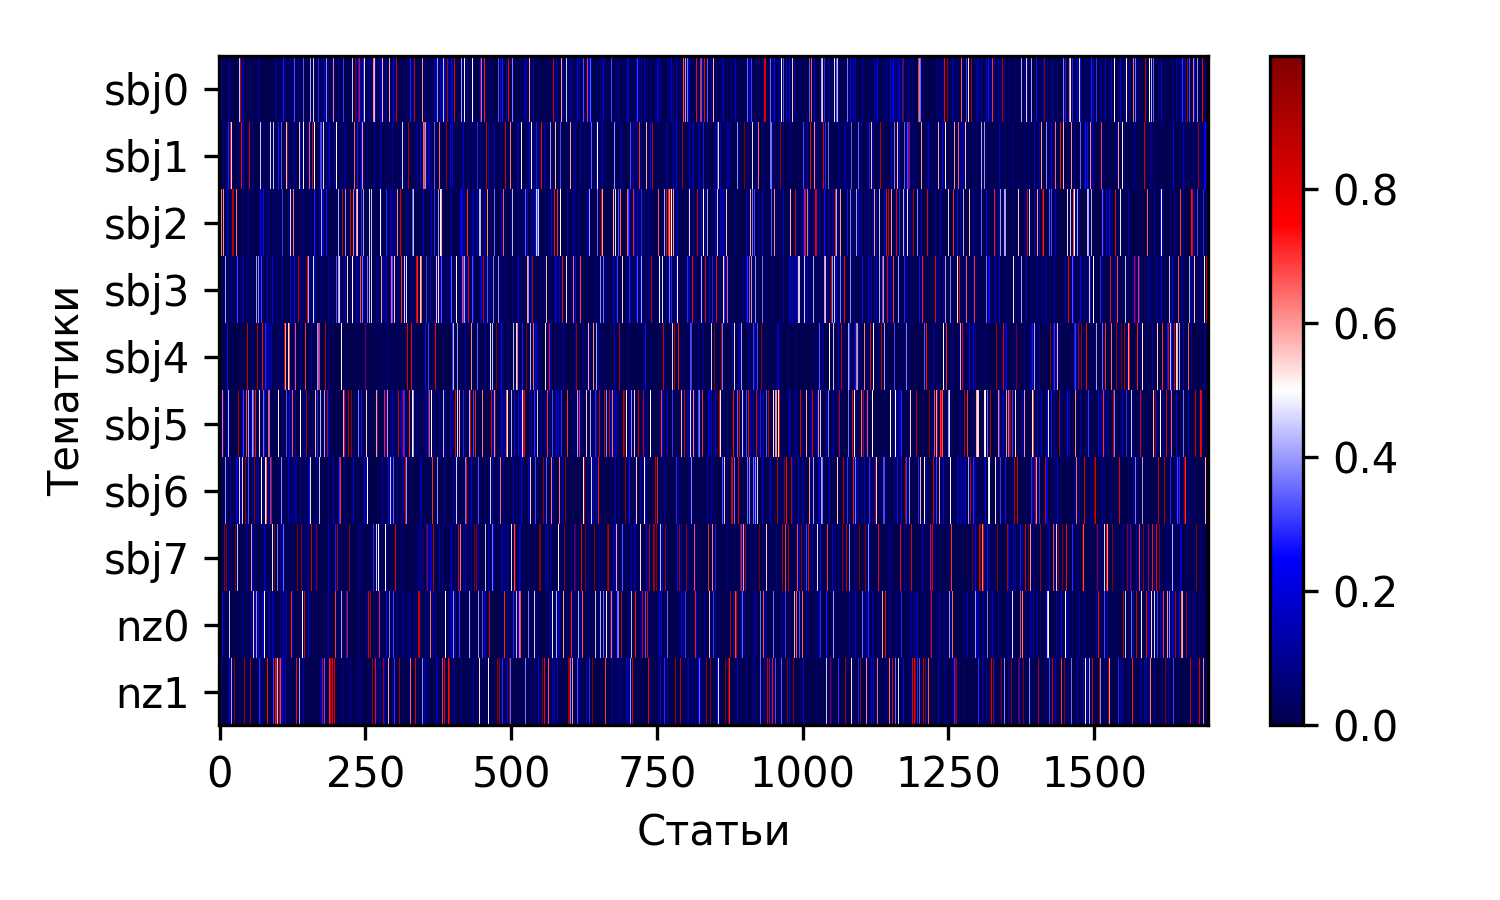
\includegraphics[width=0.8\textwidth]{op3_fig9rus}
  \label{fig:op3_9}
\end{figure}

\begin{figure}[H]
  \caption{Матрица $ \Theta $ после регуляризации. По оси x отложены номера документов из коллекции.}
  \centering
    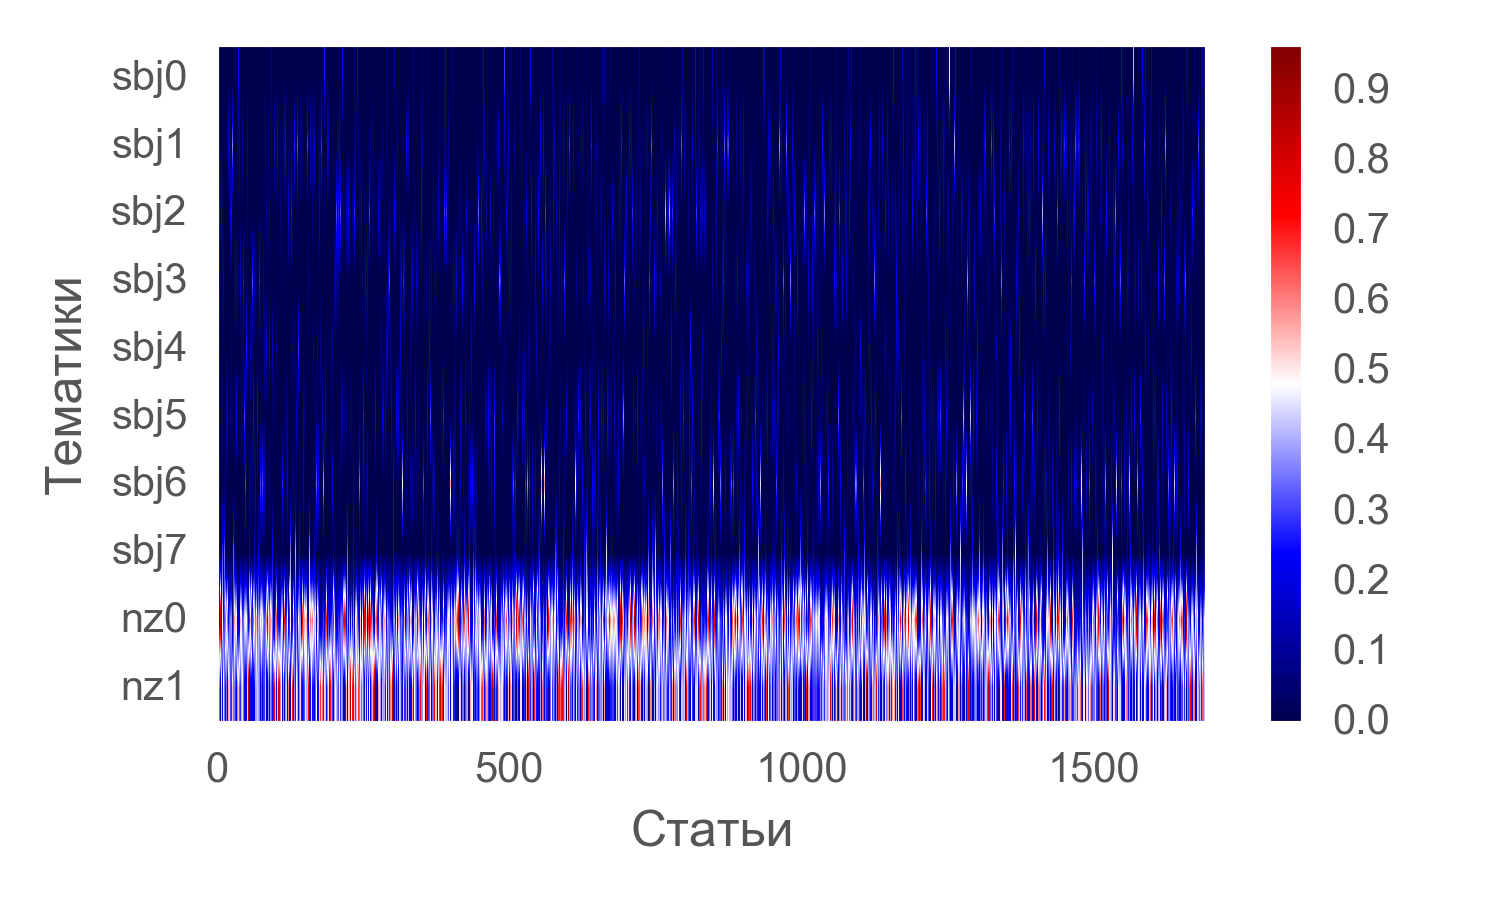
\includegraphics[width=0.8\textwidth]{op3_fig10rus}
  \label{fig:op3_10}
\end{figure}

Как мы видим из рисунков \ref{fig:op3_9} и \ref{fig:op3_10}  матрица $\Theta$ в процессе
регуляризации становится более разряженной на основных тематиках
(sbj0-sbj10) и более плотной на шумовых тематиках (nz0-nz1).

Например, документ № 555 обладает самым большим весом тематики 0.72
(sbj6). Вероятности других основных тематик для этого документа равны
нулю. Таким образом этот документ согласно модели, полностью посвящен
тематике sbj6, представленной словами
(Таб. \ref{tab:op3_2}): recovery, injection, steam,
core, viscosity, flooding, solvent, heavy, saturation, surfactant. При
помощи эксперта sbj6 дано название: ``Chemical enhanced oil recovery''.

Но с другой стороны, мы можем проверить по корпусу текстов нашей
выборки, что данный документ соответствует статье с названием ``Low
Tension Gas Process in High Salinity and Low Permeability Reservoirs''.
Вот фрагмент из публичной аннотации этой статьи с сайта
OnePetro.org\footnote{\textsuperscript{}
  https://www.onepetro.org/conference-paper/SPE-179839-MS}:


\textbf{Abstract}
\textit{Chemical enhanced oil recovery (EOR) in carbonate reservoirs has always been technically and economically challenging. Conventional Alkaline-Surfactant-Polymer (ASP) flooding has limited application in low permeability (2-20 mD) and high salinity formations (~200,000 ppm TDS) with a large concentration of divalent cations. Also  into such low permeability reservoirs can be a significant problem with polymer solutions ($\dots$).}

Как мы видим из этого общедоступного фрагмента статьи тематика
определена с высокой точностью. Но более того, из модели мы знаем, что
эта статья действительно сфокусирована на этой тематике. Приобретя
данную статью можно быть достаточно уверенным, что в ней не будет других
тематик.

Важно так же отметить, что можно было и не прибегать к помощи эксперта
для определения названия тематики sbj6, а воспользоваться тем, что
данный документ представлен единственной тематикой и взять название из аннотации статьи.

\section[Глубокий анализ текстов публикаций]{Выявление негативных отзывов о технологиях в текстах}
\label{seq:emo}
Использование искусственных нейронных сетей для анализа текстов получило развитие в середине 90-х годов в работах \cite{ng1997feature,lam1999feature,lam1999automatic}. 

Но из-за высоких требований к вычислительным ресурсам для обучения нейронных сетей оставалось академической дисциплиной.
Ускорение исследований в этом направление связано с ростом скорости вычислений и с появлением таких новых архитектур искусственных нейронных сетей как сверточные нейронные сети \cite{kim2014convolutional} и рекуррентные нейронные сети \cite{mikolov2010recurrent}.
Для обучения нейронных сетей всегда были нужны значительные массивы размеченных данных.
А с появлением большего количества слоев с нейронами потребность в размеченных данных выросла в разы. 
Для примера, чтобы обучить искусственную нейронную сеть со ста тысячью коэффициентами нужны десятки тысяч размеченных текстов. 
А для архитектуры глубоких нейронных сетей количество обучаемых коэффициентов составляет миллионы \cite{krizhevsky2012imagenet,miller1995wordnet}.
Поэтому обучение искусственной нейронной сети на собственных данных означает выделение определенного времени и ресурсов на разметку. 
Другими словами, каждый классифицируемый объект человек должен отнести к одному из классов «вручную».
Не так давно появились размеченные корпусы текстов с открытым доступом, например,
UMICH SI650 \footnote{https://www.kaggle.com/c/si650winter11} , TreeBank \footnote{http://nlp.stanford.edu/sentiment/treebank.html}, 
Twitter Sentiments \footnote{http://www.sananalytics.com/lab/twitter-sentiment/} , MPQA Opinion Corpus \cite{http://mpqa.cs.pitt.edu} и работы по их анализу \cite{maas2011learning,socher2013recursive, akkaya2009subjectivity}.

Для данного эксперимента автор применил методику Transfer learning.
В качестве размеченного набора данных автором были выбраны отзывы о кинофильмах \cite{maas2011learning}. 
В этом наборе данных содержится 25 тысяч положительных и 25 тысяч отрицательных отзывов. 
Набор данных таким образом сбалансирован для обучения и валидации модели классификации.
Длинна отзывов варьируется от 5 до 977 слов и отображена на рисунке (Рис. \ref{fig:op4_2}).
\begin{figure}[ht]
	\centering
	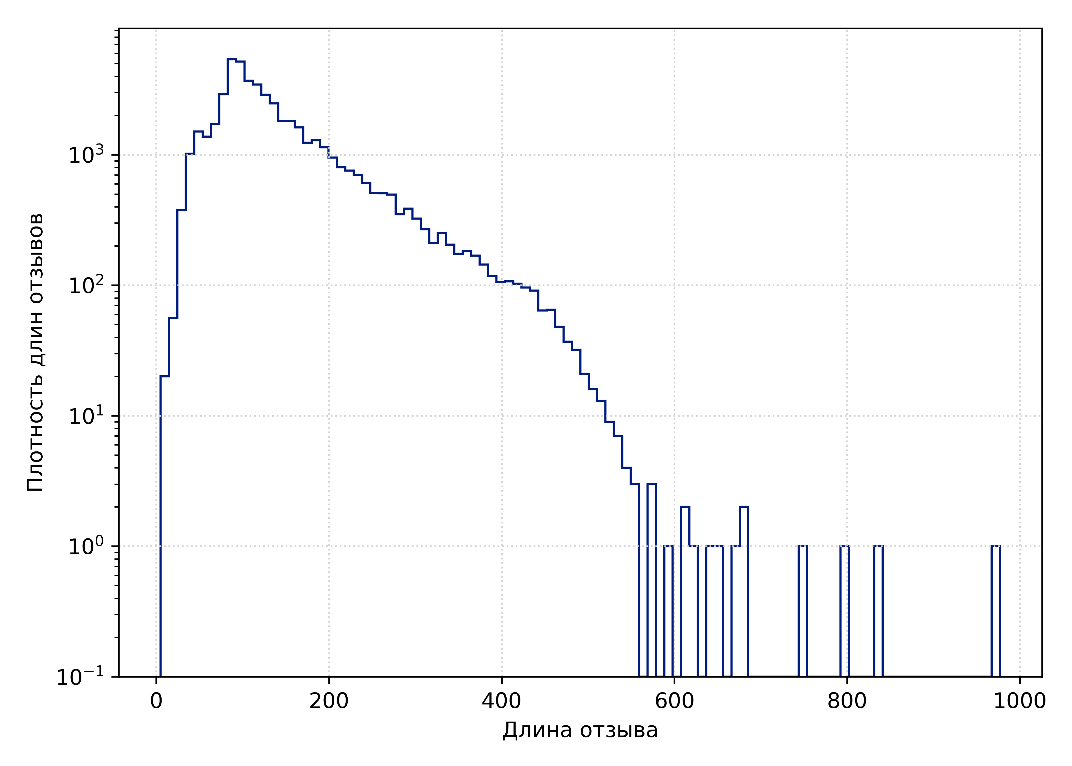
\includegraphics[width=0.8\textwidth]{op4_2}
	\caption{Распределение длин отзывов.}
	\label{fig:op4_2}
\end{figure}

При составлении словаря по отзывам были отброшены низкочастотные слова, то есть слова, встречающиеся в документах редко. Распределение частот слов по документам отображено на диаграмме (Рис. \ref{fig:op4_3} ).
\begin{figure}[ht]
  \centering
  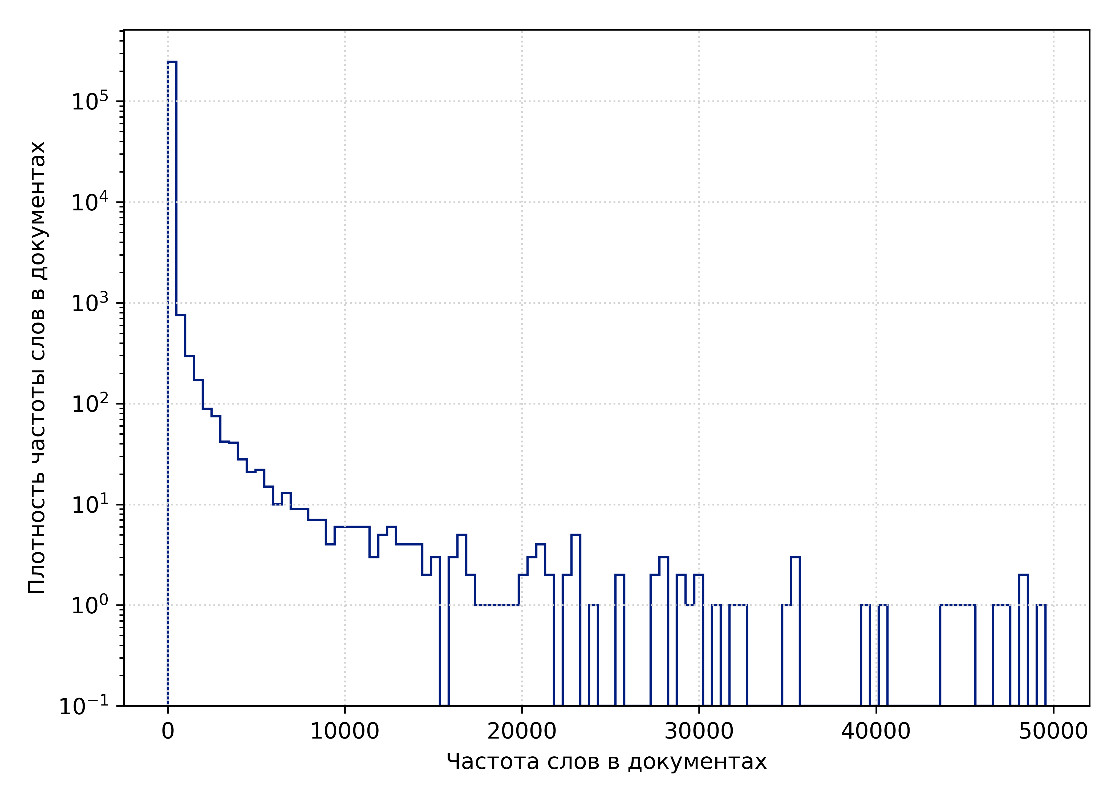
\includegraphics[width=0.8\textwidth]{op4_3}
  \caption{Распределение частот слов по документам.}
  \label{fig:op4_3}
\end{figure}

В качестве набора данных для тестирования были выбраны 1696 научно-практических статей с портала OnePetro.org.  

Для построения векторной модели текста была использована обученная модель GloVe. 
Были использованы вектора с размерностью 100 и 300. 
Преимущества от использования обученной векторной модели текста состоит в существенном сокращении объема вычислений.
Количество обучаемых параметров для создания векторной модели текста в разы превосходит количество параметров для выбранных автором архитектур моделей классификации. 

Автор ограничил себя классом моделей, построенных на основе искусственных нейронных сетей. 
Среди архитектур искусственных нейронных сетей используемых для классификации текстов можно выделить CNN-LSTM и Stacked LSTM.  
Автором были выбраны следующие три варианта архитектур моделей для классификации с использованием искусственных нейронных сетей.

\begin{enumerate}
\tightlist
\item Рекуррентная нейронная сеть из одного слоя LSTM.  Далее будем называть эту архитектуру RNN и отдельно указывать количество элементов в LSTM слое.
\item Сверточная нейронная сеть из одного слоя Dropout-Conv1D-Conv1D-MaxPooling и рекуррентная нейронная сеть из одного слоя элементов LSTM. Далее будем называть эту архитектуру CNN-LSTM и отдельно указывать количество элементов и параметры сверточных слоев.
\item Рекуррентная нейронная сеть из двух слоев LSTM. Далее будем называть эту архитектуру RNN-2 и отдельно указывать количество элементов в LSTM слое.
\end{enumerate}

Для рассматриваемых архитектур моделей классификации автор выбрал следующие существенные гиперпараметры:
\begin{itemize}
\tightlist
\item Тип модели классификации: RNN, CNN-LSTM, RNN-2.
\item Размерность словаря. В зависимости от фильтров низкочастотных слов размерность словаря изменялась от 2000 до 200000 слов.
\item Размерность векторной модели текста: 100 и 300
\item Длинна фрагмента текста: 80, 128 и 196.
\end{itemize}

Обучение моделей классификации производилось параллельно на нескольких серверах. 
Набор данных содержал равное количество положительный и отрицательных отзывов поэтому для оценки качества обучения была выбрана метрика Accuracy. 
Оптимизация параметров модели для классификации производилась на основании функции перекрестной энтропии (Cross Entropy). 
Для ускорения обучения автором был применен метод ранней остановки обучения на основании метрики Accuracy по валидационному набору данных. Кривые обучения для модели классификации типа RNN отображены на рисунках (Рис. \ref{fig:op4_4} , Рис. \ref{fig:op4_5} ).

\begin{figure}[ht]
  \centering
  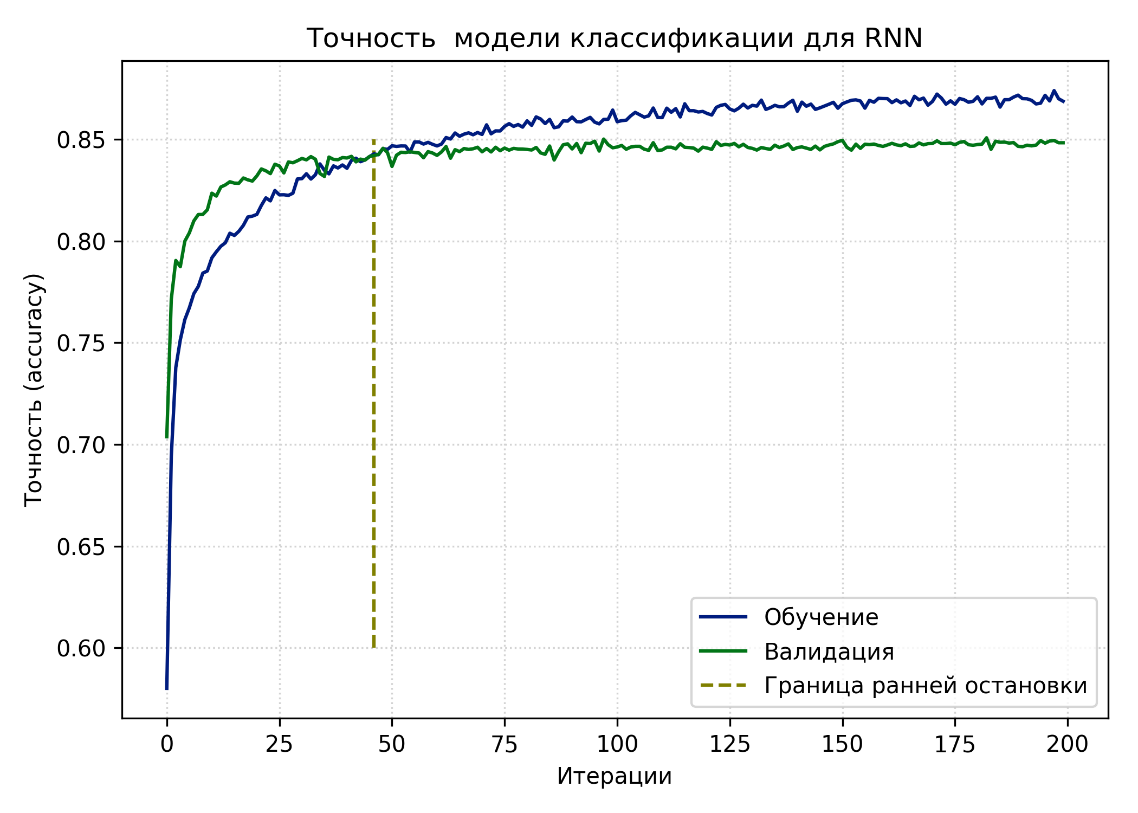
\includegraphics[width=0.8\textwidth]{op4_4}
  \caption{Кривая обучения метрики Accuracy для модели классификации типа RNN.}
  \label{fig:op4_4}
\end{figure}

Из зависимости метрики Accuracy для тренировочного и валидационного набора данных (Рис. \ref{fig:op4_4} ) видно, что в районе 42-й итерации обучения метрика Accuracy перестает увеличиваться для валидационного набора данных. 
Это явление означает, что модель начинает переучиваться по метрике Accuracy и обучение следует остановить. 
Данная архитектура модели для классификации не позволяет повышать точность на этом наборе данных.  

\begin{figure}[H]
  \caption{Кривая функции потерь для модели классификации типа RNN.}
  \centering
    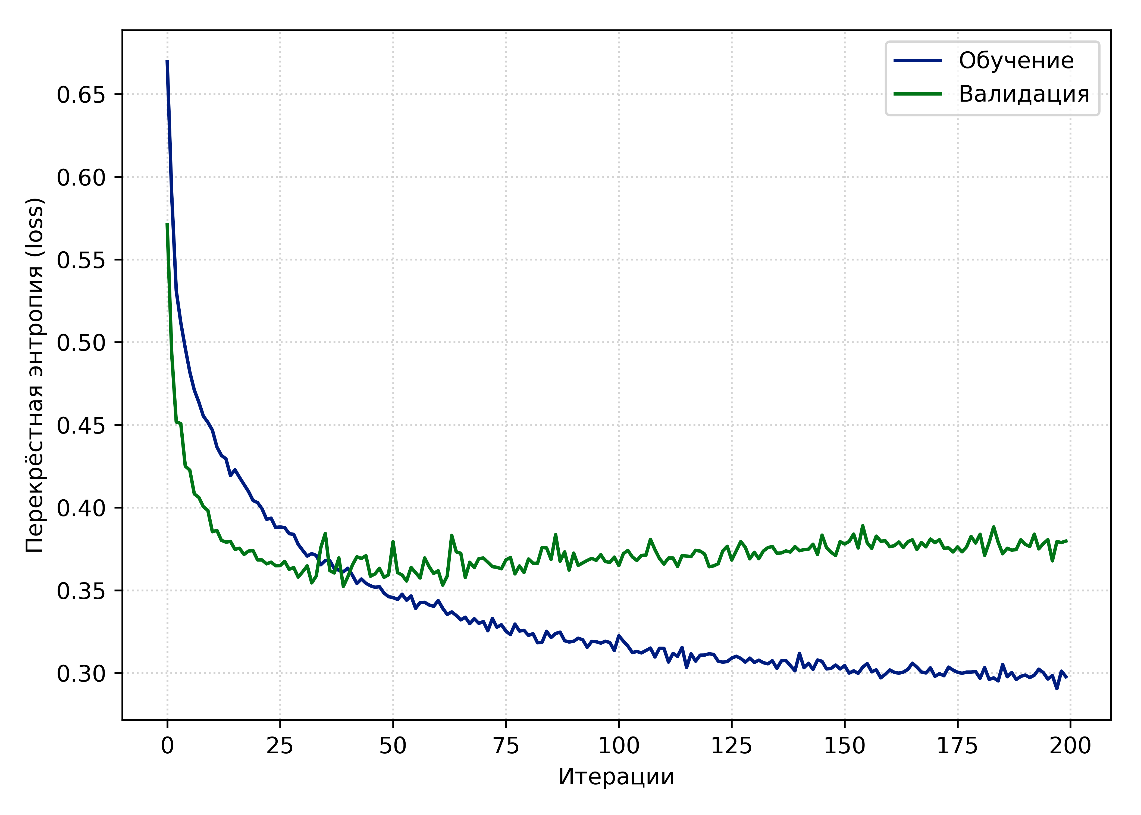
\includegraphics[width=0.8\textwidth]{op4_5}
  \label{fig:op4_5}
\end{figure}

Отметим что из зависимости, отображенной на Рис. \ref{fig:op4_5} видно, что значение перекрестной энтропии на валидационном наборе данных начинает не убывать в районе 37 итерации. 
То есть, немногим раньше, чем начинает деградировать метрика Accuracy. 

На основании изложенных выше методик было проведено обучение моделей классификации с различными архитектурами и гиперпараметрами. 
Результаты обучения приведены в таблице (Таб. \ref{tab:op4_1}).

\begin{table}[H]
\centering
\caption{Результаты обучения моделей классификации с различными гиперпараметрами.}
\label{tab:op4_1}
\resizebox{\textwidth}{!}{%
\begin{tabular}{|l|l|l|l|l|l|}
\hline
\textbf{Архитектура модели} & \textbf{Количество параметров,  тыс.} & \textbf{Длинна фрагмента текста} & \textbf{Размерность векторного пространства текста} & \textbf{Словарь, количество слов} & \textbf{Точность валидации} \\ \hline
CNN+RNN & 63 & 128 & 100 & 2 300 & 0,85 \\ \hline
CNN+RNN & 63 & 196 & 100 & 2 300 & 0,87 \\ \hline
CNN+RNN & 63 & 196 & 100 & 23 400 & 0,86 \\ \hline
RNN & 69 & 128 & 100 & 2 300 & 0,87 \\ \hline
RNN & 722 & 196 & 300 & 23 400 & 0,88 \\ \hline
RNN & 81 & 128 & 100 & 47 969 & 0,85 \\ \hline
RNN-2 & 161 & 128 & 100 & 2 300 & 0,86 \\ \hline
RNN-2 & 161 & 196 & 100 & 2 300 & 0,87 \\ \hline
RNN-2 & 1 443 & 196 & 300 & 23 000 & 0,87 \\ \hline
RNN-2 & 1 443 & 196 & 300 & 248 739 & 0,85 \\ \hline
RNN-2 & 1 443 & 80 & 300 & 248 739 & 0,85 \\ \hline
\end{tabular}%
}
\end{table}

Лучшее значение метрики Accuracy на валидационном наборе данных показала модель RNN со словарем из 23 тысяч слов и размерностью векторной модели текста равной 300. Отметим, что на тестовом наборе данных значение метрики Accuracy для данной модели составило 88\%.

Полученная модель была использована для предсказания тональности научных статей портала OnePetro.org.  Каждая научная статья разбивалась на фрагменты длинной 196 слов для оценки эмоциональной окраски. Затем фрагменты статей собирались обратно для получения эмоциональной карты всей статьи. Таким образом, можно было определить фрагменты статьи, обладающие аномальными эмоциональными окрасками, такими как разочарование и удовлетворенность. 

Данное исследование не принимает в расчет семантику текста, поэтому предмет эмоциональной окраски автоматически не определялся. Выбранные фрагменты статьи необходимо проанализировать с помощью эксперта. Но такой подход к аннотированию статьи позволил найти сложно обнаруживаемые фрагменты. В Таблице \ref{tab:op4_2} приведены примеры эмоциональных фрагментов статей.

\begin{table}[H]
\centering
\caption{Выявленные эмоциональные фрагменты статей.}
\label{tab:op4_2}
\resizebox{\textwidth}{!}{%
\begin{tabular}{|l|}
\hline
\textit{the results from pilot tests which were using as injectant are disappointing and the results from pilot tests which were using natural gases are encouraging} \\ \hline
\textit{to sum up diffusion mechanism for in pilot tests had not been well recognized which in turn did not enhance oil production rate in those wells} \\ \hline
\textit{the outstanding result from this study} \\ \hline
\textit{using the other forward model result  dramatically bad} \\ \hline
\end{tabular}%
}
\end{table}

Так же автор разработал цветовое представление эмоциональной окраски статей в зависимости от вероятности отнесения фрагмента текста к положительной или отрицательной эмоциональной окраске.

\begin{figure}[H]
  \caption{Карта полярности эмоциональной окраски статей 1696 статей. По оси x отложен порядковый номер статьи, по оси y эмоциональная окраска фрагментов статьи. На цветовой шкале отображена цифровая характеристика эмоциональности: негативная (-1), позитивная (+1).}
  \centering
    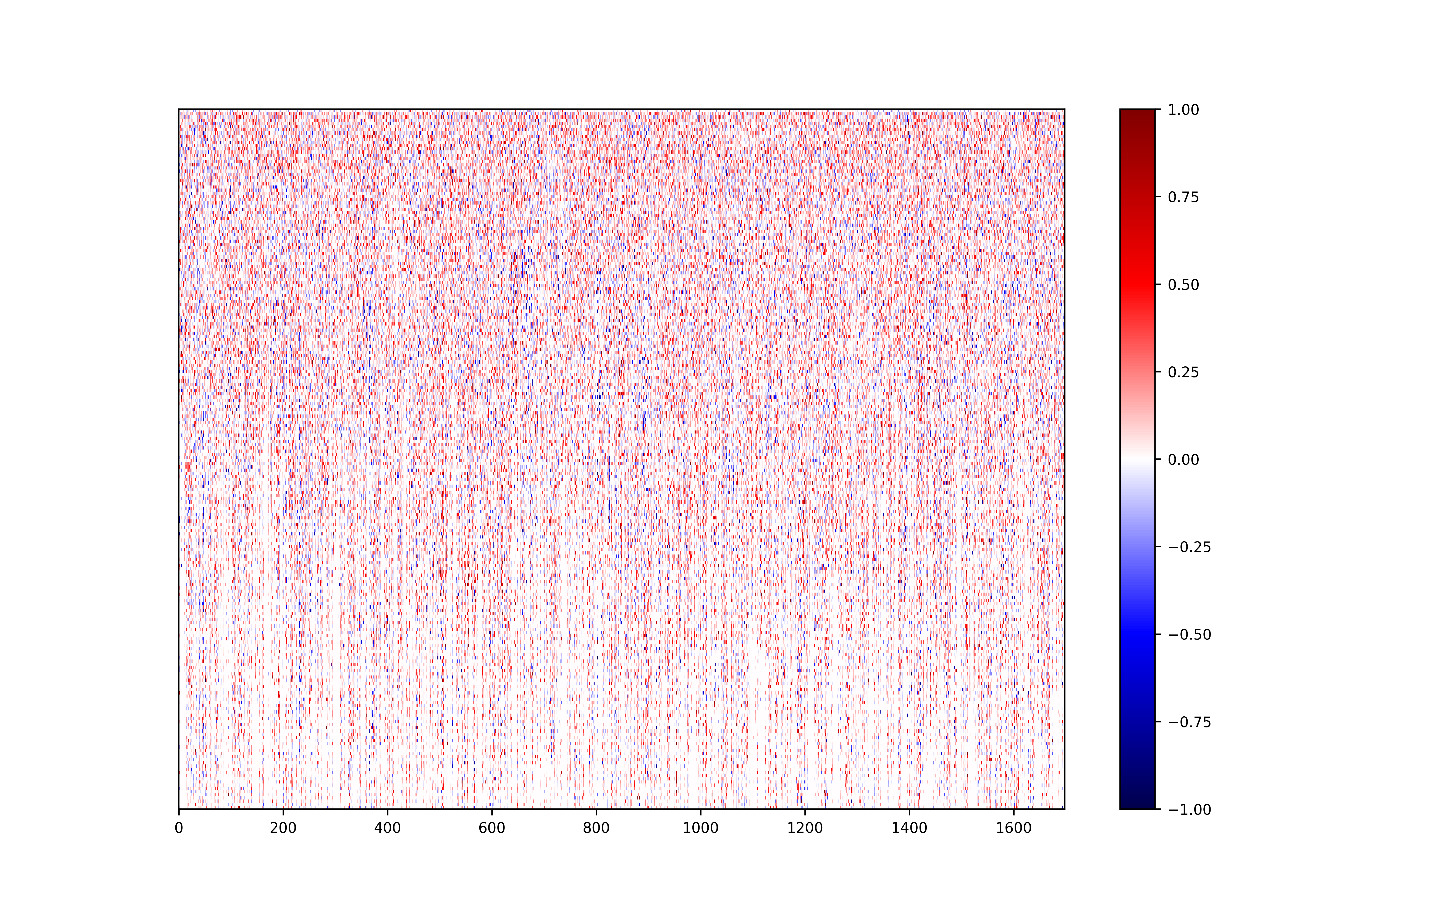
\includegraphics[width=0.8\textwidth]{op4_6}
  \label{fig:op4_6}
\end{figure}

На рисунке (Рис. \ref{fig:op4_6}) эмоциональность фрагментов статей отображена в виде карты. Для каждой статьи на оси X цветом отображена эмоциональность каждого фрагмента последовательно по оси Y. 

Научные статьи используют академическую лексику и ожидать в них градус эмоций сравнимый с отзывами на кинофильмы было бы наивно. Но современные концепции обработки текста, основанные на анализе контекста, позволяют выделять и классифицировать изменения эмоциональности достаточно точно для того, чтобы обрабатывать даже научные статьи. Автор считает, что проведенное исследование открывает возможности по созданию дополнительных инструментов для аннотации и классификации научных текстов.

